\section*{第三章 圆锥曲线}

\section*{一、曲线和方程}

\section*{【典型题型和解题技巧】}

求动点轨迹方程时应注意两点.

(1)坐标系的选取应力求“对称”.

例 1 已知线段 ${AB}$ 的长为 10 ,动点 $P$ 到点 $A,B$ 的距离平方和为 122,求动点 $P$ 的轨迹方程.

解 如图 1,建立直角坐标系,使 ${AB}$ 在 $x$ 轴上,原点为 ${AB}$ 的中点, 则点 $A,B$ 的坐标依次为 $\left( {-5,0}\right) ,\left( {5,0}\right)$ . 设动点 $P\left( {x,y}\right)$ ,则由 ${\left| PA\right| }^{2} +$  ${\left| PB\right| }^{2} = {122}$ ,得 ${\left( x + 5\right) }^{2} + {y}^{2} + {\left( x - 5\right) }^{2} + {y}^{2} = {122}$ ,化简得 ${x}^{2} + {y}^{2} = {36}$ .

\begin{center}
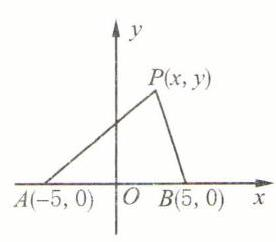
\includegraphics[width=0.2\textwidth]{bodyxb/src/bo_d20aucref24c73anc48g_56_1191_879_276_242_0.jpg}
\end{center}


(图 1)

(2)动点要具有“任意性”.

例 2 已知动点 $P$ 到直线 $x =  - 5$ 和点 $A\left( {1,0}\right)$ 的距离相等,求动点 $P$ 的轨迹方程.

分析 图 2 中把点 $P$ 标在点(-2,0)是不妥的,虽然点(-2,0)满足要求,但这一点太特殊,不具备 “任意性”; 同样,图 3 中把点 $P$ 标在 $y$ 轴上,也是不妥的,同样缺乏 “一般性”; 图 4 的标法比较合理.

\begin{center}
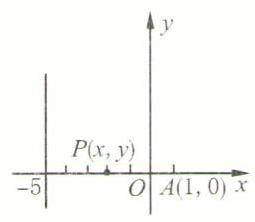
\includegraphics[width=0.2\textwidth]{bodyxb/src/bo_d20aucref24c73anc48g_56_305_1407_255_222_0.jpg}
\end{center}


(图 2)

\begin{center}
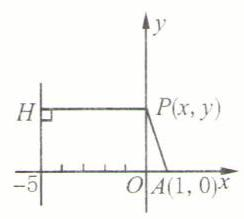
\includegraphics[width=0.2\textwidth]{bodyxb/src/bo_d20aucref24c73anc48g_56_690_1408_244_219_0.jpg}
\end{center}


(图 3)

\begin{center}
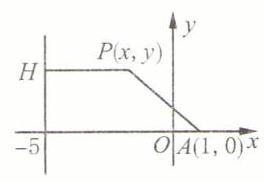
\includegraphics[width=0.2\textwidth]{bodyxb/src/bo_d20aucref24c73anc48g_56_1062_1445_264_182_0.jpg}
\end{center}


(图 4)

解 设动点为 $P\left( {x,y}\right)$ . 由 $\left| {PH}\right|  = \left| {PA}\right|$ ,得 $x + 5 = \sqrt{{\left( x - 1\right) }^{2} + {y}^{2}}$ ,化简得 ${y}^{2} = {12}\left( {x + 2}\right)$ . 【训练题】

\section*{(A)}

1. 下列各点中,在曲线 ${x}^{2} - {xy} + {2y} + 1 = 0$ 上的点是 (   )

(A)(2, - 2). (B)(4, - 3).

(C)(3,10). (D)(-2,5).

2. 方程 $4{x}^{2} - {y}^{2} + {4x} + {2y} = 0$ 表示的曲线是 (   )

(A) 一个点. (B) 两条互相平行的直线.

(C) 两条互相垂直的直线. (D) 两条相交但不垂直的直线.

3. 若曲线 $C$ 的方程是 $F\left( {x,y}\right)  = 0$ ,则曲线 $C$ 关于直线 $y = x$ 对称的曲线方程是 (   )

(A) $F\left( {y,x}\right)  = 0$ . (B) $F\left( {-y, - x}\right)  = 0$ .

(C) $F\left( {-y,x}\right)  = 0$ . (D) $F\left( {y, - x}\right)  = 0$ .

4. 若点 $M$ 到 $x$ 轴的距离和它到直线 $y = 8$ 的距离相等,则点 $M$ 的轨迹方程是(   )

(A) $x =  - 4$ . (B) $x = 4$ . (C) $y =  - 4$ . (D) $y = 4$ .

5. (1) 若两直线 $x + y = {3a},x - y = a$ 的交点在方程 ${x}^{2} + {y}^{2} = 1$ 所表示的曲线上,则 $a$ =\blkda{}；

(2)若抛物线 $y = {x}^{2} - {2x}\sin \theta  + 1\left( {0 \leq  \theta  \leq  \pi }\right)$ 的顶点在直线 $x + {2y} - 2 = 0$ 上,则 $\theta$ 的值等于\blkda{}；

(3)已知直线 ${2x} - y + k = 0$ 与曲线 ${x}^{2} + {y}^{2} - {2x} = 0$ .

①若两者仅有一个公共点,则实数 $k =$ \blkda{}；

②若两者没有公共点,则实数 $k$ 的取值范围是\blkda{}.

\section*{(B)}

6. 方程 $\left( {{2x} + y}\right) \left( {x + y - 3}\right)  = 0$ 与 $\left( {{4x} + {2y} + 1}\right) \left( {{2x} - y + 1}\right)  = 0$ 所表示的两曲线的公共点个数是(   )

(A) 1 . (B) 2 .

(C) 3 . (D) 多于 3 个.

7. 已知坐标满足方程 $F\left( {x,y}\right)  = 0$ 的点都在曲线 $C$ 上,则下列命题正确的是 (   )

(A) 曲线 $C$ 上的点的坐标都适合方程 $F\left( {x,y}\right)  = 0$ .

(B) 不在 $C$ 上的点的坐标必不适合方程 $F\left( {x,y}\right)  = 0$ .

(C) 凡坐标不适合方程 $F\left( {x,y}\right)  = 0$ 的点都不在 $C$ 上.

(D) 不在 $C$ 上的点的坐标有些适合方程 $F\left( {x,y}\right)  = 0$ .

8. 直线 ${2x} + {3y} - 6 = 0$ 关于点(1, - 1)对称的直线的方程是(   )

(A) ${3x} - {2y} + 2 = 0$ . (B) ${2x} + {3y} + 8 = 0$ .

(C) ${3x} - {2y} + {12} = 0$ . (D) ${2x} - {3y} + 8 = 0$ .

9. 曲线 $f\left( {x,y}\right)  = 0$ 关于直线 $x - y - 2 = 0$ 对称的曲线方程为 (   )

(A) $f\left( {y + 2,x}\right)  = 0$ . (B) $f\left( {x - 2,y}\right)  = 0$ .

(C) $f\left( {y + 2,x - 2}\right)  = 0$ . (D) $f\left( {y - 2,x + 2}\right)  = 0$ .

10. (1) 求抛物线 $y = {x}^{2} - {2x} - 1$ 在 $x$ 轴上截得的线段长;

(2)求直线 $y = x + 3$ 被抛物线 $y = 2{x}^{2}$ 截得的线段长.

11. 设 $k \in  \mathbf{R}$ ,试讨论直线 $y = x + k$ 与曲线 $4{x}^{2} + 9{y}^{2} = {36}$ 的公共点个数.

12. 已知函数 $y = \dfrac{x - 1}{{ax} - 1}\left( {x \in  \mathbf{R}}\right.$ 且 $x \neq  \dfrac{1}{a}$ ,其中 $a$ 为实常数,且 $a \neq  0,a \neq  1$ ),求证:

(1)经过这个函数图像上任意两个不同的点的直线不平行于 $x$ 轴；

(2)这个函数的图像关于直线 $y = x$ 成轴对称图形.

13. 求直线 $l : {ax} - y + b = 0$ 经过两直线 ${l}_{1} : {2x} - {2y} - 3 = 0$ 与 ${l}_{2} : {3x} - {5y} + 1 = 0$ 交点的充要条件, 并证明你的结论.

\section*{二、圆}

\section*{(一) 圆的标准方程和一般方程}

\section*{【典型题型和解题技巧】}

1. 求圆的方程.

例 1 求过点 $A\left( {2, - 3}\right) ,B\left( {-2, - 5}\right)$ ,且圆心在直线 $x - {2y} - 3 = 0$ 上的圆的方程.

解 如图 5, $\because$ 圆心在直线 $x - {2y} - 3 = 0$ 上,故可设圆心为 $M\left( {{2b} + 3,b}\right)$ ,再由 $\left| {MA}\right|  =$  $\left| {MB}\right|$ ,得 ${\left\lbrack  \left( 2b + 3\right)  - 2\right\rbrack  }^{2} + {\left( b + 3\right) }^{2} = {\left\lbrack  \left( 2b + 3\right)  + 2\right\rbrack  }^{2} + {\left( b + 5\right) }^{2}$ ,整理得 $b =  - 2$ ,于是圆心为 $M( - 1$ , $- 2)$ ,半径为 $\left| {MA}\right|  = \sqrt{{\left( 2 + 1\right) }^{2} + {\left( -3 + 2\right) }^{2}} = \sqrt{10}$ .

\begin{center}
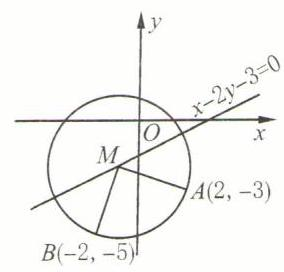
\includegraphics[width=0.2\textwidth]{bodyxb/src/bo_d20aucref24c73anc48g_58_1194_1095_284_272_0.jpg}
\end{center}


(图 5)

$\therefore$ 所求的圆的方程为 ${\left( x + 1\right) }^{2} + {\left( y + 2\right) }^{2} = {10}$ .

2. 点和圆的位置关系.

对于点 $P\left( {{x}_{0},{y}_{0}}\right)$ 和圆 ${\left( x - a\right) }^{2} + {\left( y - b\right) }^{2} = {r}^{2}$ ,有

${\left( {x}_{0} - a\right) }^{2} + {\left( {y}_{0} - b\right) }^{2} > {r}^{2} \Leftrightarrow$ 点在圆外,

${\left( {x}_{0} - a\right) }^{2} + {\left( {y}_{0} - b\right) }^{2} = {r}^{2} \Leftrightarrow$ 点在圆上,

${\left( {x}_{0} - a\right) }^{2} + {\left( {y}_{0} - b\right) }^{2} < {r}^{2} \Leftrightarrow$ 点在圆内.

例 2 已知抛物线 $y = {x}^{2} + {2x} + b$ 与 $x$ 轴交于 $A,B$ 两点,以 ${AB}$ 为直径作圆 (如图 6),求:

(1) $b$ 的取值范围;

\begin{center}
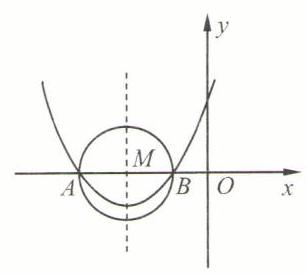
\includegraphics[width=0.2\textwidth]{bodyxb/src/bo_d20aucref24c73anc48g_58_1173_1563_307_275_0.jpg}
\end{center}


(图 6)

(2)圆的方程；

(3) $b$ 的取值范围,使抛物线的顶点在圆的内部.

解 (1) 令 $y = 0$ ,得 ${x}^{2} + {2x} + b = 0$ . 由 $\Delta  = 4 - {4b} > 0$ ,得 $b < 1$ .

(2)设圆心为 $M\left( {{x}_{0},0}\right)$ ,显然点 $M$ 在抛物线的对称轴上,

$\therefore {x}_{0} =  - 1$ ,故圆心为 $M\left( {-1,0}\right)$ .

设 $A\left( {{x}_{1},0}\right) ,B\left( {{x}_{2},0}\right)$ ,则 ${x}_{1},{x}_{2}$ 是方程 ${x}^{2} + {2x} + b = 0$ 的两根.

由 ${\left| AB\right| }^{2} = {\left( {x}_{2} - {x}_{1}\right) }^{2} = {\left( {x}_{1} + {x}_{2}\right) }^{2} - 4{x}_{1}{x}_{2} = {\left( -2\right) }^{2} - {4b} = 4 - {4b}$ ,

得圆的半径为 $\left| {MA}\right|  = \sqrt{1 - b}$ ,故所求的圆的方程为 ${\left( x + 1\right) }^{2} + {y}^{2} = 1 - b\left( {b < 1}\right)$ .

(3)抛物线的顶点为(-1, b - 1),依题意,应有 ${\left( -1 + 1\right) }^{2} + {\left( b - 1\right) }^{2} < 1 - b$ ,

即 ${b}^{2} - b < 0,\therefore 0 < b < 1$ .

\section*{(A)}

14. 圆 ${x}^{2} + {y}^{2} - {6x} + {4y} = 0$ 的周长是(   )

(A) $\sqrt{13}\pi$ . (B) $2\sqrt{13}\pi$ . (C) ${2\pi }$ . (D) $2\sqrt{3}\pi$ .

15. 两圆 ${x}^{2} + {y}^{2} + {2mx} + {m}^{2} - 1 = 0$ 与 ${x}^{2} + {y}^{2} + {2mx} + {2y} + {m}^{2} + {2m} = 0$ 的圆心距是 (   )

(A) 1 . (B) $\sqrt{2}$ . (C) $2\left| m\right|$ . (D) $2 - {2m}$ .

16. 过点 $P\left( {-8, - 1}\right) ,Q\left( {5,{12}}\right) ,R\left( {{17},4}\right)$ 三点的圆的圆心坐标是 (   )

(A) $\left( {\dfrac{14}{3},5}\right)$ . (B)(5,1). (C)(0,0). (D)(5, - 1).

17. 已知方程 ${x}^{2} + {y}^{2} + {2kx} + {4y} + {3k} + 8 = 0$ 表示一个圆,则实数 $k$ 的取值范围是 ( )

(A) $k >  - \dfrac{8}{3}$ . (B) $k <  - \dfrac{8}{3}$ .

(C) $- 1 < k < 4$ . (D) $k <  - 1$ 或 $k > 4$ .

18. 若两直线 $y = x + {2k}$ 与 $y = {2x} + k + 1$ 的交点 $P$ 在圆 ${x}^{2} + {y}^{2} = 4$ 的内部,则 $k$ 的取值范围是(   )

(A) $- \dfrac{1}{5} < k <  - 1$ . (B) $- \dfrac{1}{5} < k < 1$ .

(C) $- \dfrac{1}{3} < k < 1$ . (D) $- 2 < k < 2$ .

19. 若圆 ${x}^{2} + {y}^{2} + {4x} + {2by} + {b}^{2} = 0$ 与两坐标轴都相切,则 $b$ 的值所组成的集合是 (   )

(A) $\{  - 2,2\}$ . (B) $\{ 1,2\}$ . (C) $\{  - 1, - 2\}$ . (D) $\{  - 1,1\}$ .

20. (1)若方程 ${x}^{2} + {y}^{2} - x + y + m = 0$ 表示圆,则实数 $m$ 的取值范围是\blkda{}；

(2)若方程 ${a}^{2}{x}^{2} + \left( {{2a} + 3}\right) {y}^{2} + {2ax} + a + 1 = 0$ 表示圆,则实数 $a$ 的值等于\blkda{}；

(3)若两直线 $x - {2y} - {2k} = 0$ 与 ${2x} - {3y} - k = 0$ 的交点在圆 ${x}^{2} + {y}^{2} = {36}$ 上,则实数 $k$ 的值等于\blkda{}.

21. 已知圆的方程为 ${\left( x - a\right) }^{2} + {\left( y - b\right) }^{2} = {r}^{2}\left( {r > 0}\right)$ ,试根据下列条件,分别写出 $a,b,r$ 应满足的条件:

(1)圆心在 $x$ 轴上:\blkda{}； (2)圆与 $y$ 轴相切:\blkda{}；

(3)圆过原点且与 $y$ 轴相切:\blkda{}； (4)圆与两坐标轴均相切:\blkda{}；

(5)原点在圆内:\blkda{}； (6)圆与 $x$ 轴相交:\blkda{}.

22. 根据条件,写出圆的标准方程:

(1)以 $A\left( {-1,2}\right) ,B\left( {5, - 6}\right)$ 为直径两端点的圆；

(2)过两点 $\left( {3,5}\right) ,\left( {-3,7}\right)$ ,且圆心在 $x$ 轴上的圆；

(3)圆心在直线 ${2x} - y = 3$ 上,且与两坐标轴相切的圆；

(4)过点 $M\left( {5,2}\right) ,N\left( {3,2}\right)$ 且圆心在直线 $y = {2x} - 3$ 上的圆.

\section*{(B)}

23. 两圆 ${x}^{2} + {y}^{2} + {2kx} + {k}^{2} - 1 = 0$ 与 ${x}^{2} + {y}^{2} + 2\left( {k + 1}\right) y + {k}^{2} + {2k} = 0$ 圆心间的最短距离是(   )

(A) $2\sqrt{2}$ . (B) $\sqrt{2}$ . (C) 1 . (D) $\dfrac{\sqrt{2}}{2}$ .

24. 方程 ${x}^{4} - {y}^{4} - 4{x}^{2} + 4{y}^{2} = 0$ 所表示的曲线是(   )

(A) 两条相交的直线. (B) 两条相交直线和两条平行直线.

(C) 两条平行直线和一个圆. (D) 两条相交直线和一个圆.

25. 若圆 ${x}^{2} + {y}^{2} + {dx} + {ey} + f = 0$ 与两坐标轴都相切,则常数 $d,e,f$ 之间的关系是 (   )

(A) $d \neq  0$ 且 ${e}^{2} = {4f}$ . (B) $d \neq  0$ 且 ${e}^{2} \neq  {4f}$ .

(C) $d = e$ 且 ${e}^{2} \neq  {4f}$ . (D) ${d}^{2} = {e}^{2} = {4f} > 0$ .

26. 已知圆 ${x}^{2} + {y}^{2} + {mx} + {ny} + p = 0$ 与 $x$ 轴相切于原点,则 $m,n,p$ 应满足(   )

(A) ${mn} \neq  0$ 且 $p = 0$ . (B) $m \neq  0$ 且 ${n}^{2} + {p}^{2} = 0$ .

(C) $n \neq  0$ 且 ${m}^{2} + {p}^{2} = 0$ . (D) $p \neq  0$ 且 ${m}^{2} + {n}^{2} = 0$ .

27. 若圆 ${x}^{2} + {y}^{2} - {4x} + {2y} + m = 0$ 与 $y$ 轴交于 $A,B$ 两点,且 $\angle {AMB} = {90}^{ \circ  }$ (其中 $M$ 为已知圆的圆心),则 $m$ 等于(   )

(A) -3. (B) 3. (C) 8. (D) $2\sqrt{2}$ .

28. 方程 $\left| x\right|  - 1 = \sqrt{1 - {\left( y - 1\right) }^{2}}$ 所表示的曲线是 (   )

(A) 一个圆. (B) 两个圆.

(C) 半个圆. (D) 两个半圆.

29. 方程组 $\left\{  \begin{array}{l} {x}^{2} - {y}^{2} = 0, \\  {x}^{2} + {y}^{2} + {2ax} + {a}^{2} - 1 = 0 \end{array}\right.$ 有四个不同实数解的充要条件是 (   )

(A) $a \in  \left( {0,1}\right)$ .

(B) $a \in  \left( {-1,1}\right)$ .

(C) $a \in  \left( {-\sqrt{2}, - 1}\right)  \cup  \left( {-1,1}\right)  \cup  \left( {1,\sqrt{2}}\right)$ .

(D) $a \in  \left( {-\sqrt{2}, - 1}\right)  \cup  \left( {-1,0}\right)  \cup  \left( {0,1}\right)  \cup  \left( {1,2}\right)$ .

30. (1) 求圆 ${x}^{2} + {y}^{2} + {Dx} + {Ey} + F = 0\left( {{D}^{2} + {E}^{2} - {4F} > 0}\right)$ 关于直线 $x + y = 0$ 对称的充要条件;

(2)求圆 ${x}^{2} + {y}^{2} - {2x} + {6y} + 9 = 0$ 关于直线 $x + y = 0$ 对称的圆的方程；

(3) 求圆 ${x}^{2} + {y}^{2} - {4y} = 0$ 关于直线 $x - y + 1 = 0$ 对称的圆的方程;

(4)求圆 ${x}^{2} + {y}^{2} - x + {2y} = 0$ 关于直线 $x - y + 1 = 0$ 对称的圆的方程.

\section*{(二) 直线和圆}

\section*{【典型题型和解题技巧】}

1. 直线和圆位置关系的判定.

判定直线 ${ax} + {by} + c = 0$ 和圆 ${\left( x - {x}_{0}\right) }^{2} + {\left( y - {y}_{0}\right) }^{2} = {R}^{2}$ 位置关系的方法有两种:

(1)比较圆心 $\left( {{x}_{0},{y}_{0}}\right)$ 到直线 ${ax} + {by} + c = 0$ 的距离 $d$ 和圆半径 $R$ 的大小.

(2)从方程组 $\left\{  \begin{array}{l} {ax} + {by} + c = 0, \\  {\left( x - {x}_{0}\right) }^{2} + {\left( y - {y}_{0}\right) }^{2} = {R}^{2} \end{array}\right.$ 中消去变量 $y\left( {\text{ 或 }x}\right)$ ,得到关于 $x\left( {\text{ 或 }y}\right)$ 的二次方程 $A{x}^{2} + {Bx} + C = 0$ (或 $A{y}^{2} + {By} + C = 0$ ),考察根的判别式 $\Delta$ 的情况. 容易证明以下结论:

$d < R \Leftrightarrow$ 相交 $\Leftrightarrow  \Delta  > 0$ ;

$d = R \Leftrightarrow$ 相切 $\Leftrightarrow  \Delta  = 0$ ;

$d > R \Leftrightarrow$ 相离 $\Leftrightarrow  \Delta  < 0$ .

注意 判断直线和圆的位置关系,一般来说,比较 $d$ 和 $R$ 的大小的方法比利用 $\Delta$ 来判定的方法要显得优越.

例 1 求实数 $m$ ,分别使直线 $x - {my} + 3 = 0$ 和圆 ${x}^{2} + {y}^{2} - {6x} + 5 = 0$ :

(1)相交; (2)相切; (3) 相离.

解 圆的方程即为 ${\left( x - 3\right) }^{2} + {y}^{2} = 4$ ,圆心(3,0)到直线 $x - {my} + 3 = 0$ 的距离 $d = \dfrac{6}{\sqrt{{m}^{2} + 1}}$ .

(1)要直线与圆相交,则 $d < R$ ,即 $\dfrac{6}{\sqrt{{m}^{2} + 1}} < 2$ ,得 $m <  - 2\sqrt{2}$ 或 $m > 2\sqrt{2}$ .

(2)要直线与圆相切,则 $d = R$ ,即 $\dfrac{6}{\sqrt{{m}^{2} + 1}} = 2$ ,得 $m =  \pm  2\sqrt{2}$ .

(3)要直线与圆相离,则 $d > R$ ,即 $\dfrac{6}{\sqrt{{m}^{2} + 1}} > 2$ ,得 $- 2\sqrt{2} < m < 2\sqrt{2}$ .

2. 直线和圆相交的题型.

对于直线和圆相交的问题, 通常利用两种途径求解:

(1)利用垂径定理和勾股定理.

\begin{center}
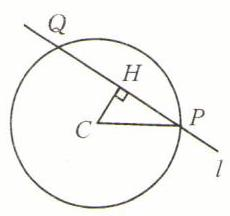
\includegraphics[width=0.2\textwidth]{bodyxb/src/bo_d20aucref24c73anc48g_61_1203_1654_230_216_0.jpg}
\end{center}


(图 7)

解题途径主要是从图形的性质考虑. 设直线 $l$ 和圆 $C$ 交于 $P,Q$ 两点,作 ${CH} \bot  l,H$ 为垂足 (如图 7),连接 ${CP}$ ,则 $H$ 为 ${PQ}$ 的中点,且 ${\left| CH\right| }^{2} +$  ${\left| PH\right| }^{2} = {\left| CP\right| }^{2}.$ (2)利用韦达定理. 解题途径主要是从方程的性质考虑.

设直线和圆交于点 $P\left( {{x}_{1},{y}_{1}}\right) ,Q\left( {{x}_{2},{y}_{2}}\right)$ ,从方程组 $\left\{  \begin{array}{l} {ax} + {by} + c = 0, \\  {\left( x - {x}_{0}\right) }^{2} + {\left( y - {y}_{0}\right) }^{2} = {R}^{2} \end{array}\right.$ 中消去 $y$ (或 $x$ ),得二次方程 $A{x}^{2} + {Bx} + C = 0$ . (或 $A{y}^{2} + {By} + C = 0$ ).

由韦达定理得 $\left\{  \begin{array}{l} {x}_{1} + {x}_{2} =  - \dfrac{B}{A}, \\  {x}_{1} \cdot  {x}_{2} = \dfrac{C}{A}, \end{array}\right.$ 或 $\left\{  \begin{array}{l} {y}_{1} + {y}_{2} =  - \dfrac{B}{A}, \\  {y}_{1} \cdot  {y}_{2} = \dfrac{C}{A} \end{array}\right.$ ,且 $\bigtriangleup   = {B}^{2} - {4AC} > 0$ .

例 2 求直线 ${2x} - y - 1 = 0$ 被圆 ${x}^{2} + {y}^{2} - {2y} - 1 = 0$ 所截得的弦的长.

\begin{center}
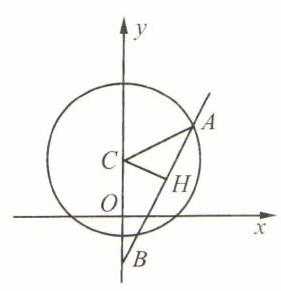
\includegraphics[width=0.2\textwidth]{bodyxb/src/bo_d20aucref24c73anc48g_62_1175_329_281_291_0.jpg}
\end{center}


(图 8)

解 已知圆即为 ${x}^{2} + {\left( y - 1\right) }^{2} = 2$ ,圆心为 $C\left( {0,1}\right)$ ,半径 $R = \sqrt{2}$ (如图 8),点 $C$ 到直线的距离 $\left| {CH}\right|  = \dfrac{\left| -1 - 1\right| }{\sqrt{5}} = \dfrac{2}{\sqrt{5}}$ ,

故弦长 $\left| {AB}\right|  = 2\left| {AH}\right|  = 2\sqrt{{\left| AC\right| }^{2} - {\left| CH\right| }^{2}} = 2\sqrt{2 - \dfrac{4}{5}}$

$= \dfrac{2\sqrt{30}}{5}$ .

例 3 已知圆 ${x}^{2} + {y}^{2} + x - {6y} + m = 0$ 和直线 $x + {2y} - 3 = 0$ 交于 $P,Q$ 两点. 若 ${OP} \bot  {OQ}$ ( $O$ 是原点,如图 9),求 $m$ 的值.

解 由方程组 $\left\{  \begin{array}{l} x + {2y} - 3 = 0, \\  {x}^{2} + {y}^{2} + x - {6y} + m = 0, \end{array}\right.$

\begin{center}
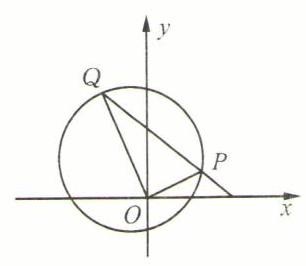
\includegraphics[width=0.2\textwidth]{bodyxb/src/bo_d20aucref24c73anc48g_62_1154_937_306_266_0.jpg}
\end{center}


(图 9)

消去 $x$ ,得 $5{y}^{2} - {20y} + {12} + m = 0$ .

设 $P\left( {{x}_{1},{y}_{1}}\right) ,Q\left( {{x}_{2},{y}_{2}}\right)$ ,则 $\left\{  \begin{array}{l} {y}_{1} + {y}_{2} = 4, \\  {y}_{1} \cdot  {y}_{2} = \dfrac{{12} + m}{5}, \\  \Delta  = {20}^{2} - {20}\left( {{12} + m}\right)  > 0, \end{array}\right.$

而 ${x}_{1} \cdot  {x}_{2} = \left( {3 - 2{y}_{1}}\right) \left( {3 - 2{y}_{2}}\right)  = 9 - 6\left( {{y}_{1} + {y}_{2}}\right)  + 4{y}_{1}{y}_{2}$

$= 9 - {24} + \dfrac{{48} + {4m}}{5} = \dfrac{{4m} - {27}}{5}.$

由 ${OP} \bot  {OQ}$ ,得 ${x}_{1}{x}_{2} + {y}_{1}{y}_{2} = 0$ ,即 $\dfrac{{12} + m}{5} + \dfrac{{4m} - {27}}{5} = 0$ ,解得 $m = 3$ .

易知,当 $m = 3$ 时,上述方程的 $\Delta  > 0$ ,故 $m = 3$ .

3. 圆的切线的求法.

求圆的切线通常有三种方法:

(1) 利用 $d = R$ .

当圆 ${\left( x - a\right) }^{2} + {\left( y - b\right) }^{2} = {R}^{2}\left( {R > 0}\right)$ 的圆心(a, b)到直线 ${Ax} + {By} + C = 0$ 的距离 $d$ 等于圆的半径 $R$ 时,直线与圆相切.

例 4 已知直线 $l : y = k\left( {x - 2}\right)  + 4$ 与曲线 $C : y = 1 + \sqrt{4 - {x}^{2}}$ 有两个不同的公共点,求实数 $k$ 的取值范围.

解 由 $y = 1 + \sqrt{4 - {x}^{2}}$ 得 ${x}^{2} + {\left( y - 1\right) }^{2} = 4\left( {y \geq  1}\right)$ ,故曲线 $C$ 是一个半圆 (如图 10);

而直线 $l$ 过定点 $A\left( {2,4}\right)$ . 过点 $A$ 引半圆的切线 ${AB}$ (切点为 $B$ ). 设半圆的左端点为 $C\left( {-2,1}\right)$ ,按题目要求,直线 $l$ 应夹在直线 ${AB}$ 与 ${AC}$ 之间,故 $k$ 的取值应在 ${k}_{AC}$ 与 ${k}_{AB}$ 之间.

\begin{center}
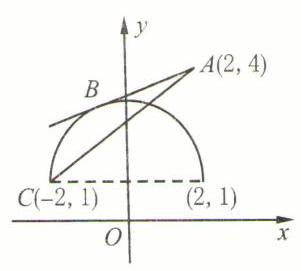
\includegraphics[width=0.2\textwidth]{bodyxb/src/bo_d20aucref24c73anc48g_63_1080_138_301_271_0.jpg}
\end{center}


(图 10)

$\because {k}_{AC} = \dfrac{4 - 1}{2 + 2} = \dfrac{3}{4}$ ,再由半圆的圆心(0,1)到直线 ${kx} - y + 4 - {2k}$  $= 0$ 的距离 $d = \dfrac{\left| 2k - 3\right| }{\sqrt{{k}^{2} + 1}} = 2$ ,得 $k = \dfrac{5}{12}$ . 故 $k$ 的取值范围是 $\left( {\dfrac{5}{12},\dfrac{3}{4}}\right\rbrack$ .

(2)利用 $\Delta  = 0$ .

从所设的切线方程与圆方程中消去 $y\left( {\text{ 或 }x}\right)$ ,得一元二次方程,然后利用 $\Delta  = 0$ 解之.

(3)利用切线公式.

可利用的公式有:

(i) 切点为 $\left( {{x}_{0},{y}_{0}}\right)$ ,则圆 ${x}^{2} + {y}^{2} = {R}^{2}$ 的切线为 ${x}_{0}x + {y}_{0}y = {R}^{2}$ ; 切点为 $\left( {{x}_{0},{y}_{0}}\right)$ ,则圆 ${\left( x - a\right) }^{2} + {\left( y - b\right) }^{2} = {R}^{2}$ 的切线为 $\left( {x - a}\right) \left( {{x}_{0} - a}\right)  + \left( {y - b}\right) \left( {{y}_{0} - b}\right)  = {R}^{2}$ [公式证明见第 52 (1)题];

(ii) 斜率为 $k$ ,则圆 ${x}^{2} + {y}^{2} = {R}^{2}$ 的切线为: $y = {kx} \pm  R\sqrt{{k}^{2} + 1}$ .

例 5 已知实数 $x,y$ 满足 ${x}^{2} + {y}^{2} = 1$ ,求 $\dfrac{y + 2}{x + 1}$ 的取值范围.

解 如图 11,设 $P\left( {x,y}\right)$ 是圆 ${x}^{2} + {y}^{2} = 1$ 上的点,则 $\dfrac{y + 2}{x + 1}$ 是表示过点 $P\left( {x,y}\right) ,A\left( {-1, - 2}\right)$ 两点的直线 ${PA}$ 的斜率.

\begin{center}
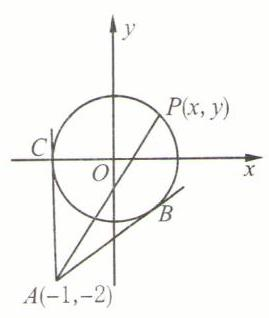
\includegraphics[width=0.2\textwidth]{bodyxb/src/bo_d20aucref24c73anc48g_63_1116_1121_269_318_0.jpg}
\end{center}


(图 11)

过点 $A$ 作圆的切线 ${AB}$ 和 ${AC}$ ,易见 ${AC} \bot  x$ 轴,因此, ${k}_{PA} \geq  {k}_{AB}$ .

设圆 ${x}^{2} + {y}^{2} = 1$ 过点 $A\left( {-1, - 2}\right)$ 的切线 ${AB}$ 的方程为 $y + 2 =$  $k\left( {x + 1}\right)$ ,则圆心(0,0)到 ${AB}$ 的距离 $\dfrac{\left| k - 2\right| }{\sqrt{{k}^{2} + 1}} = 1$ ,由此得 $k = \dfrac{3}{4}$ ,

$\therefore \dfrac{y + 2}{x + 1}$ 的取值范围是 $\left\lbrack  {\dfrac{3}{4}, + \infty }\right)$ .

4. 圆的标点法.

解析几何中有一类问题常常涉及曲线上的点. 当点在直线上时,我们已经介绍了 “直线标点法”,当点在圆上时,就要用到“圆的标点法”.

对于圆 ${\left( x - a\right) }^{2} + {\left( y - b\right) }^{2} = {R}^{2}\left( {R > 0}\right)$ 上的点 $P$ ,表示的方法有两种:

(1) 设点 $P\left( {{x}_{0},{y}_{0}}\right)$ ,且 ${\left( {x}_{0} - a\right) }^{2} + {\left( {y}_{0} - b\right) }^{2} = {R}^{2}$ .

\begin{center}
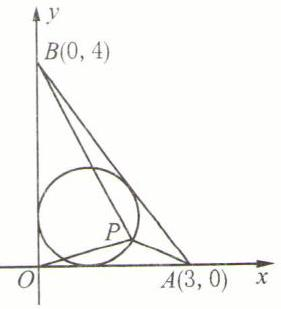
\includegraphics[width=0.2\textwidth]{bodyxb/src/bo_d20aucref24c73anc48g_63_1135_1802_281_309_0.jpg}
\end{center}


(图 12)

这种“标点法”的优越性是标法简单, 但是带着一个方程.

例 6 如图 12,已知定点 $A\left( {3,0}\right)$ 和 $B\left( {0,4}\right) ,P$ 是 $\bigtriangleup {AOB}$ 内切圆上的动点 $\left( {O\text{ 是坐标原点 }}\right)$ ,求 ${\left| PA\right| }^{2} + {\left| PB\right| }^{2} + {\left| PO\right| }^{2}$ 的最大值、最小值.

解 由已知, $\left| {AO}\right|  = 3,\left| {BO}\right|  = 4$ ,则 $\left| {AB}\right|  = 5$ . 设 $\bigtriangleup {AOB}$ 的内切圆半. 径为 $R$ ,则 $R = \dfrac{\left| {AO}\right|  + \left| {BO}\right|  - \left| {AB}\right| }{2} = \dfrac{3 + 4 - 5}{2} = 1$ .

故 $\bigtriangleup {AOB}$ 的内切圆方程为 ${\left( x - 1\right) }^{2} + {\left( y - 1\right) }^{2} = 1$ .

设圆上点为 $P\left( {{x}_{0},{y}_{0}}\right)$ ,则 ${\left( {x}_{0} - 1\right) }^{2} + {\left( {y}_{0} - 1\right) }^{2} = 1$ ,

即 ${x}_{0}^{2} + {y}_{0}^{2} - 2{x}_{0} - 2{y}_{0} + 1 = 0$ .

而 ${\left| PA\right| }^{2} + {\left| PB\right| }^{2} + {\left| PO\right| }^{2} = {\left( {x}_{0} - 3\right) }^{2} + {y}_{0}^{2} + {x}_{0}^{2} + {\left( {y}_{0} - 4\right) }^{2} + {x}_{0}^{2} + {y}_{0}^{2}$

$= 3{x}_{0}^{2} + 3{y}_{0}^{2} - 6{x}_{0} - 8{y}_{0} + {25} = 3\left( {{x}_{0}^{2} + {y}_{0}^{2} - 2{x}_{0} - 2{y}_{0} + 1}\right)  + {22} - 2{y}_{0} = {22} - 2{y}_{0},$

显然 $0 \leq  {y}_{0} \leq  2,\therefore {\left| PA\right| }^{2} + {\left| PB\right| }^{2} + {\left| PO\right| }^{2}$ 的最大值是 22,最小值是 18.

(2)设点 $P\left( {a + R\cos \theta ,b + R\sin \theta }\right)$ .

这种“标点法”的缺陷是标法不够简单, 它的优越性在于不带方程.

有兴趣的读者不妨以此种“标点法”求解例 6.

\section*{【训练题】}

\section*{(A)}

31. 直线 ${5x} + {12y} - 8 = 0$ 与圆 ${\left( x - 1\right) }^{2} + {\left( y + 3\right) }^{2} = 8$ 的位置关系是 (   )

(A) 相交且直线过圆心. (B) 相切.

(C) 相交但直线不过圆心. (D) 相离.

32. 若直线 ${4x} - {3y} - 2 = 0$ 与圆 ${x}^{2} + {y}^{2} - {2ax} + {4y} + {a}^{2} - {12} = 0$ 总有两个不同的公共点,则 $a$ 的取值范围是(   )

(A) $- 3 < a < 7$ . (B) $- 6 < a < 4$ . (C) $- 7 < a < 3$ . (D) $- {21} < a < {19}$ .

33. 圆 ${\left( x - 3\right) }^{2} + {\left( y - 3\right) }^{2} = 9$ 上到直线 ${3x} + {4y} - {11} = 0$ 的距离等于 1 的点有(   )

(A) 1 个. (B) 2 个. (C) 3 个. (D) 4 个.

34. 圆 ${\left( x - 2\right) }^{2} + {\left( y + 3\right) }^{2} = 2$ 上与点(0, - 5)的距离最大的点的坐标是 (   )

(A)(5,1). (B)(3, - 2).

(C)(4,1). (D) $\left( {\sqrt{2} + 2,\sqrt{2} - 3}\right)$ .

35. 若直线 $x + y = r$ 与圆 ${x}^{2} + {y}^{2} = r\left( {r > 0}\right)$ 相切,则实数 $r$ 的值等于 (   )

(A) $\dfrac{\sqrt{2}}{2}$ . (B) 1 . (C) $\sqrt{2}$ . (D) 2 .

36. (1) $P\left( {3,0}\right)$ 是圆 ${x}^{2} + {y}^{2} - {8x} - {2y} + {12} = 0$ 内一点,在过点 $P$ 的弦中,最长的弦所在的直线方程是\blkda{},最短的弦所在的直线方程是\blkda{}；

(2)圆 ${x}^{2} + {y}^{2} - {4x} - 5 = 0$ 的弦 ${AB}$ 以 $P\left( {3,1}\right)$ 为中点,则直线 ${AB}$ 的方程是\blkda{}

\blkda{}；

(3)直线 $y = {3x} + 1$ 与曲线 ${x}^{2} + {y}^{2} = 4$ 相交于 $A,B$ 两点,则弦 ${AB}$ 的中点坐标是\blkda{}.

37. (1) 直线 $x - y - 1 = 0$ 被圆 ${x}^{2} + {y}^{2} = 4$ 截得的弦长为\blkda{};

(2)当圆 ${x}^{2} + {y}^{2} - {2ax} + {2ay} + 3{a}^{2} - {2a} - 1 = 0$ 的半径最大时,这个圆在 $y$ 轴上截得的弦长等于\blkda{}；

(3) 若以 $O\left( {2, - 1}\right)$ 为圆心的圆被直线 $x - y - 1 = 0$ 截得的弦长为 $2\sqrt{2}$ ,则该圆的方程为\blkda{}；

(4)直线 $l$ 过点 $P\left( {0,2}\right)$ ,且被圆 ${x}^{2} + {y}^{2} = 4$ 所截得的弦长为 2,则 $l$ 的斜率为\blkda{}.

38. (1)自点 $M\left( {1,3}\right)$ 向圆 ${x}^{2} + {y}^{2} = 1$ 引切线,则切线长等于\blkda{}；

(2)过点 $P\left( {-3,4}\right)$ 与圆 ${x}^{2} + {y}^{2} = {25}$ 相切的切线方程为\blkda{}.

\section*{(B)}

39. 直线 $x - y + 4 = 0$ 被圆 ${x}^{2} + {y}^{2} + {4x} - {4y} + 6 = 0$ 截得的弦长等于(   )

(A) $\sqrt{2}$ . (B) 2 . (C) $2\sqrt{2}$ . (D) $4\sqrt{2}$ .

40. 已知实数 $a,b,c$ 满足 $3\left( {{a}^{2} + {b}^{2}}\right)  = 4{c}^{2}\left( {c \neq  0}\right)$ ,则直线 ${ax} + {by} + c = 0$ 与圆 ${x}^{2} + {y}^{2} = 1$ 的位置关系是(   )

(A) 相离. (B) 相切.

(C) 相交但直线不过圆心. (D) 相交且直线过圆心.

41. 已知直线 ${ax} + {by} - {ab} = 0\left( {{ab} \neq  0}\right)$ 与圆 ${x}^{2} + {y}^{2} = 1$ 相切,则下列关系正确的是 (   )

(A) $\left( {{a}^{2} - 1}\right) \left( {{b}^{2} - 1}\right)  < 1$ . (B) $\left( {{a}^{2} - 1}\right) \left( {{b}^{2} - 1}\right)  = 1$ .

(C) $\left( {{a}^{2} - 1}\right) \left( {{b}^{2} - 1}\right)  > 1$ . (D) $\left( {{a}^{2} - 1}\right) \left( {{b}^{2} - 1}\right)  = 0$ .

42. 圆 ${x}^{2} + {y}^{2} - {2x} = 3$ 与直线 $y = {ax} + 1$ 的公共点个数是 (   )

(A) 0 . (B) 1 . (C) 2 . (D) 不能确定.

43. 若 $P\left( {{x}_{0},{y}_{0}}\right)$ 是圆 ${x}^{2} + {y}^{2} = {r}^{2}$ 内异于原点的一点,则直线 ${x}_{0}x + {y}_{0}y = {r}^{2}$ 和这个圆的公共点个数是(   )

(A) 0 . (B) 1 . (C) 2 . (D) 不能确定.

44. 若实数 $x,y$ 满足 ${x}^{2} + {y}^{2} = 1$ ,则 $\dfrac{y - 2}{x - 1}$ 的最小值等于 (   )

(A) $\dfrac{1}{4}$ . (B) $\dfrac{3}{4}$ . (C) $\dfrac{\sqrt{3}}{2}$ . (D) 2 .

45. 已知直线 $y = x + m$ 与曲线 $y = \sqrt{1 - {x}^{2}}$ 有两个不同的公共点,则实数 $m$ 的取值范围是(   )

(A) $\left( {-\sqrt{2},\sqrt{2}}\right)$ . (B) $\left( {0,\sqrt{2}}\right)$ . (C) $\left( {1,\sqrt{2}}\right)$ . (D) $\lbrack 1,\sqrt{2})$ .

46. 过点 $P\left( {1,2}\right)$ 的直线 $l$ 将圆 ${x}^{2} + {y}^{2} - {4x} - 5 = 0$ 分成两个弓形,当大、小两个弓形的面积之差最大时,直线 $l$ 的方程是 (   )

(A) $x = 1$ . (B) $y = 2$ . (C) $x - y + 1 = 0$ . (D) $x - {2y} + 3 = 0$ .

47. 若集合 $A = \left\{  {\left( {x,y}\right) \left| {y =  - }\right| x \mid   - 2}\right\}  ,B = \left\{  {\left( {x,y}\right) \left| {{\left( x - a\right) }^{2} + {y}^{2} = {a}^{2}}\right. }\right\}$ 满足 $A \cap  B = \varnothing$ ,求实数 $a$ 的取值范围.

48. 已知定圆 ${x}^{2} + {y}^{2} = 8$ 和定点 $P\left( {4,0}\right)$ ,过点 $P$ 作直线 $l$ ,分别求 $l$ 的倾斜角 $\theta$ 的取值范围, 使得直线 $l$ 与已知圆:

(1) 相切; (2)相交; (3) 相离.

49. (1) 已知圆心在直线 $x - {3y} = 0$ 上的圆 $C$ 与 $y$ 轴相切,且在直线 $y = x$ 上截得的弦长为 $2\sqrt{7}$ ,求此圆的方程;

(2)求过圆 ${x}^{2} + {y}^{2} + {2x} - {4y} - 5 = 0$ 和直线 ${2x} + y + 4 = 0$ 的公共点,且面积最小的圆的方程;

(3)过点 $M\left( {3,0}\right)$ 作直线 $l$ 与圆 ${x}^{2} + {y}^{2} = {16}$ 交于 $A,B$ 两点,求 $l$ 的倾斜角 $\theta$ ,使 $\bigtriangleup  {AOB}$ 的面积最大,并求此最大值 ( $O$ 为坐标原点).

50. (1) 求和直线 ${3x} - {2y} + 4 = 0$ 垂直且与圆 ${x}^{2} - {2x} + {y}^{2} - 3 = 0$ 相切的切线方程;

(2)求过点(3,1)且与圆 ${x}^{2} - {2x} + {y}^{2} - 3 = 0$ 相切的切线方程；

(3)自点 $P\left( {-3,3}\right)$ 发出的光线 $l$ 经 $x$ 轴反射,其反射光线所在的直线与圆 ${x}^{2} + {y}^{2} - {4x} -$  ${4y} + 7 = 0$ 相切,求光线 $l$ 所在直线的方程.

51. 根据条件,求圆 $C$ 的方程:

(1)圆 $C$ 的圆心在直线 $y =  - {4x}$ 上,且与直线 $x + y - 1 = 0$ 切于点 $P\left( {3, - 2}\right)$ ；

(2)圆 $C$ 和直线 $x - {6y} - {10} = 0$ 相切于点 $Q\left( {4, - 1}\right)$ ,且经过点 $M\left( {9,6}\right)$ ；

(3) 圆 $C$ 过点(2, - 1),圆心在直线 ${2x} + y = 0$ 上,且与直线 $x - y - 1 = 0$ 相切.

52. (1) 求证:过圆 ${\left( x - a\right) }^{2} + {\left( y - b\right) }^{2} = {R}^{2}$ 上一点 $P\left( {{x}_{0},{y}_{0}}\right)$ 的切线方程是 $\left( {{x}_{0} - a}\right) \left( {x - a}\right)  +$  $\left( {{y}_{0} - b}\right) \left( {y - b}\right)  = {R}^{2}$ ;

(2)求与圆 ${\left( x - 3\right) }^{2} + {\left( y + 1\right) }^{2} = {13}$ 切于点 $A\left( {1,2}\right)$ 的直线方程.

53. (1) 已知 $P\left( {{x}_{0},{y}_{0}}\right)$ 是圆 ${x}^{2} + {y}^{2} = {r}^{2}$ 外一点,自点 $P$ 引圆的两条切线, $A,B$ 是切点,求证: 过两切点的弦 ${AB}$ 所在直线的方程是 ${x}_{0}x + {y}_{0}y = {r}^{2}$ ;

(2) $P\left( {3, - 4}\right)$ 是圆 ${x}^{2} + {y}^{2} = 4$ 外一点, ${PA}$ , ${PB}$ 是圆的切线,求切点弦 ${AB}$ 所在直线的方程.

54. (1) 在圆 ${x}^{2} + {y}^{2} = 4$ 上求一点 $P$ ,使点 $P$ 到直线 ${4x} + {3y} = 2$ 的距离最大;

(2)若点 $P\left( {x,y}\right)$ 在圆 ${\left( x - 3\right) }^{2} + {\left( y - \sqrt{3}\right) }^{2} = 6$ 上运动,求 $\dfrac{y}{x}$ 的最大值.

55. $m$ 为何实数值时,曲线 $C : {x}^{2} + {y}^{2} = 3\left( {x \geq  0}\right)$ 与直线 $l : y = m\left( {x + 1}\right)  - 3$ 有:

(1)一个公共点? (2)两个不同公共点?

56. (1) 已知实数 $x,y$ 满足 ${x}^{2} + {y}^{2} - {2x} + {4y} - {20} = 0$ ,求 ${x}^{2} + {y}^{2}$ 的最小值;

(2)若实数 $x,y$ 满足 ${x}^{2} + {y}^{2} - {2x} + {4y} = 0$ ,求 $x - {2y}$ 的最大值；

(3)已知定点 $A\left( {-1,0}\right) ,B\left( {1,0}\right)$ 和圆 ${\left( x - 3\right) }^{2} + {\left( y - 4\right) }^{2} = 4$ 上的动点 $P$ ,求使 ${\left| PA\right| }^{2} +$  ${\left| PB\right| }^{2}$ 最小时点 $P$ 的坐标.

\section*{(三) 两圆的位置关系}

\section*{【典型题型和解题技巧】}

1. 两圆位置关系的判断.

假设圆 ${C}_{1}$ 的圆心是 ${O}_{1}$ ,半径是 ${r}_{1}$ ,圆 ${C}_{2}$ 的圆心是 ${O}_{2}$ ,半径是 ${r}_{2},{r}_{1} > {r}_{2}$ ,那么:

$\left| {{O}_{1}{O}_{2}}\right|  > {r}_{1} + {r}_{2} \leftrightarrow$ 两圆外离[如图 13(1)];

$\left| {{O}_{1}{O}_{2}}\right|  = {r}_{1} + {r}_{2} \Leftrightarrow$ 两圆外切[如图 13(2)];

${r}_{1} - {r}_{2} < \left| {{O}_{1}{O}_{2}}\right|  < {r}_{1} + {r}_{2} \Leftrightarrow$ 两圆相交[如图 13(3)];

$\left| {{O}_{1}{O}_{2}}\right|  = {r}_{1} - {r}_{2} \Leftrightarrow$ 两圆内切[如图 13(4)];

$\left| {{O}_{1}{O}_{2}}\right|  < {r}_{1} - {r}_{2} \Leftrightarrow$ 两圆内含 [如图 13(5)].

\begin{center}
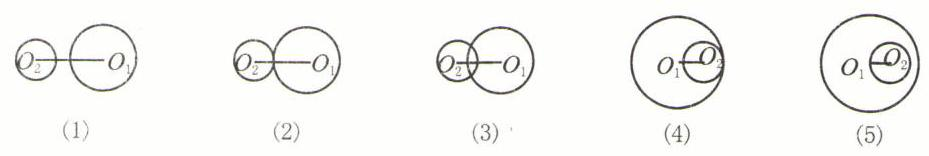
\includegraphics[width=0.7\textwidth]{bodyxb/src/bo_d20aucref24c73anc48g_67_271_380_929_156_0.jpg}
\end{center}


(图 13)

例 1 两圆 ${C}_{1} : {x}^{2} + {y}^{2} + {2x} - {6y} - {26} = 0$ 与 ${C}_{2} : {x}^{2} + {y}^{2} - {4x} + {2y} + 4 = 0$ 的公切线有(   )

(A) 1 条. (B) 2 条. (C) 3 条. (D) 4 条.

解 ’. 圆 ${C}_{1} : {\left( x + 1\right) }^{2} + {\left( y - 3\right) }^{2} = {36}$ ,圆 ${C}_{2} : {\left( x - 2\right) }^{2} + {\left( y + 1\right) }^{2} = 1$ ,

$\therefore {O}_{1}\left( {-1,3}\right) ,{r}_{1} = 6,{O}_{2}\left( {2, - 1}\right) ,{r}_{2} = 1$ ,

于是 ${r}_{1} - {r}_{2} = 5,\left| {{O}_{1}{O}_{2}}\right|  = \sqrt{{\left( 2 + 1\right) }^{2} + {\left( -1 - 3\right) }^{2}} = 5$ ,

$\therefore \left| {{O}_{1}{O}_{2}}\right|  = {r}_{1} - {r}_{2}$ ,

故两圆内切, 因此公切线只有 1 条, 答案应选 A.

2. 两相交圆的“根轴”.

如图 14,若两圆 ${C}_{1} : {x}^{2} + {y}^{2} + {D}_{1}x + {E}_{1}y + {F}_{1} = 0$ 和圆 ${C}_{2} : {x}^{2} + {y}^{2} +$  ${D}_{2}x + {E}_{2}y + {F}_{2} = 0$ 相交于两点 $A,B$ ,则称直线 ${AB}$ 为这两圆的“根轴”. 容易证明,“根轴”的方程是 $\left( {{D}_{1} - {D}_{2}}\right) x + \left( {{E}_{1} - {E}_{2}}\right) y + \left( {{F}_{1} - {F}_{2}}\right)  = 0$ .

\begin{center}
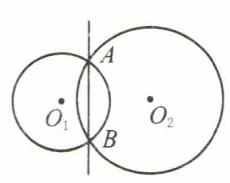
\includegraphics[width=0.2\textwidth]{bodyxb/src/bo_d20aucref24c73anc48g_67_1158_1131_230_183_0.jpg}
\end{center}


(图 14)

例 2 已知两圆 ${x}^{2} + {y}^{2} - {10x} - {10y} = 0$ 和 ${x}^{2} + {y}^{2} + {6x} - {2y} - {40} = 0$ , 求:(1)它们的公共弦所在的直线方程；(2)公共弦长.

解(1) $\because$ 圆 ${C}_{1} : {\left( x - 5\right) }^{2} + {\left( y - 5\right) }^{2} = {50}$ ,圆心 ${O}_{1}\left( {5,5}\right)$ ,半径 ${r}_{1} = 5\sqrt{2}$ ,

圆 ${C}_{2} : {\left( x + 3\right) }^{2} + {\left( y - 1\right) }^{2} = {50}$ ,圆心 ${O}_{2}\left( {-3,1}\right)$ ,半径 ${r}_{2} = 5\sqrt{2}$ ,

于是 ${r}_{1} - {r}_{2} < \left| {{O}_{1}{O}_{2}}\right|  < {r}_{1} + {r}_{2}$ ,两圆相交.

\begin{center}
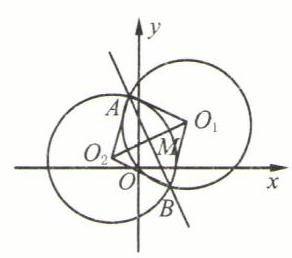
\includegraphics[width=0.2\textwidth]{bodyxb/src/bo_d20aucref24c73anc48g_67_1092_1549_292_258_0.jpg}
\end{center}


(图 15)

$\therefore$ 公共弦 ${AB}$ 所在直线的方程为 ${16x} + {8y} - {40} = 0$ ,

即 ${2x} + y - 5 = 0$ .

(2)如图 15,连接 ${O}_{1}A,{O}_{1}B,{O}_{2}A,{O}_{2}B$ ,显然 ${O}_{1}A{O}_{2}B$ 是菱形, 故 ${AB}$ 与 ${O}_{1}{O}_{2}$ 互相垂直平分于点 $M$ ,又 $\left| {{O}_{1}{O}_{2}}\right|  = \sqrt{{64} + {16}} = 4\sqrt{5}$ ,

$\therefore \left| {{O}_{1}M}\right|  = 2\sqrt{5}$ ,而 $\left| {{O}_{1}A}\right|  = 5\sqrt{2}$ ,故 $\left| {AM}\right|  = \sqrt{{50} - {20}} = \sqrt{30}$ ,于是公共弦的长 $\left| {AB}\right|  = 2\sqrt{30}$ .

\section*{(A)}

57. 与两圆 ${x}^{2} + {y}^{2} + {4x} - {4y} + 7 = 0$ 和 ${x}^{2} + {y}^{2} - {4x} - {10y} + {13} = 0$ 都相切的直线有 (   )

(A) 1 条. (B) 2 条. (C) 3 条. (D) 4 条.

58. 两圆 ${x}^{2} + {y}^{2} - {8x} + {6y} - {11} = 0$ 与 ${x}^{2} + {y}^{2} = {100}$ 的位置关系是 (   )

(A) 相离. (B) 相交. (C) 外切. (D) 内切.

59. 若半径为 1,圆心为(0, b)的圆和定圆 ${\left( x - 1\right) }^{2} + {\left( y - 2\right) }^{2} = 1$ 相切,则 $b$ 的值等于 (   )

(A) $\pm  \sqrt{3}$ . (B) $2 \pm  \sqrt{3}$ . (C) $1 \pm  \sqrt{3}$ . (D) $1 \pm  2\sqrt{3}$ .

60. (1) 若两圆 ${\left( x - a\right) }^{2} + {y}^{2} = 1$ 与 ${x}^{2} + {\left( y - b\right) }^{2} = 1$ 外切,则实数 $a,b$ 之间应满足的关系式是\blkda{}；

(2)以 $A\left( {1, - 2}\right)$ 为圆心,与圆 ${x}^{2} + {y}^{2} = {45}$ 相切的圆的方程是\blkda{}；

(3) 设 $0 < \alpha  < \dfrac{\pi }{2}$ ,则两圆 ${\left( x + \dfrac{1}{2}\right) }^{2} + {y}^{2} = \dfrac{1}{16}$ 和 ${\left( x - \sin \alpha \right) }^{2} + {\left( y - 1\right) }^{2} = \dfrac{1}{16}$ 的位置关系是\blkda{}；

(4)若两圆 ${x}^{2} + {y}^{2} = 9$ 与 ${x}^{2} + {y}^{2} - {4ax} - {2y} + 4{a}^{2} - 3 = 0$ 相切,则实数 $a =$ \blkda{}.

\section*{(B)}

61. 两圆 ${x}^{2} + {y}^{2} + {2ax} + {2ay} + 2{a}^{2} - 1 = 0$ 与 ${x}^{2} + {y}^{2} + {2bx} + {2by} + 2{b}^{2} - 2 = 0$ 的公共弦长的最大值是(   )

(A) $2\sqrt{2}$ . (B) 2 . (C) $\sqrt{2}$ . (D) 1 .

62. 已知集合 $M = \left\{  {\left( {x,y}\right)  \mid  {x}^{2} + {y}^{2} \leq  4}\right\}$ 与 $N = \left\{  {\left( {x,y}\right)  \mid  {\left( x - 1\right) }^{2} + {\left( y - 1\right) }^{2} \leq  {r}^{2}\left( {r > 0}\right) }\right\}$ 满足 $M \cap  N = N$ ,则 $r$ 的取值范围是 (   )

(A) $\left( {0,\sqrt{2} - 1}\right\rbrack$ . (B) $(0,1\rbrack$ .

(C) $\left( {0,2 - \sqrt{2}}\right\rbrack$ . (D) $(0,2\rbrack$ .

63. (1) 已知两圆 ${x}^{2} + {y}^{2} + {4x} - {4y} - 1 = 0$ 与 ${x}^{2} + {y}^{2} + {2x} + {2y} - 2 = 0$ 相交于 $P,Q$ 两点,则公共弦 ${PQ}$ 的垂直平分线的方程是\blkda{}；

(2)两圆 ${x}^{2} + {y}^{2} + {4x} - {4y} = 0$ 与 ${x}^{2} + {y}^{2} - x = 0$ 的公共弦所在的直线方程为\blkda{}；

(3)两圆 ${x}^{2} + {y}^{2} - {10x} - {10y} = 0$ 与 ${x}^{2} + {y}^{2} + {6x} + {2y} - {40} = 0$ 的公共弦长为\blkda{}.

64. 若两圆 ${x}^{2} + {y}^{2} = m$ 与 ${x}^{2} + {y}^{2} + {6x} - {8y} - {11} = 0$ 有公共点,求实数 $m$ 的取值范围.

65. 根据下列条件, 求圆的一般方程:

(1)以两圆 ${\left( x - a\right) }^{2} + {y}^{2} = {r}^{2}$ 和 ${x}^{2} + {y}^{2} = {r}^{2}$ 的公共弦为直径的圆；

(2)以两圆 ${x}^{2} + {y}^{2} + {4x} + {2y} + 1 = 0$ 与 ${x}^{2} + {y}^{2} + {2x} + {2y} - 2 = 0$ 的公共弦为直径的圆；

(3)过点 $P\left( {4, - 1}\right)$ 且与已知圆 ${x}^{2} + {y}^{2} + {2x} - {6y} + 5 = 0$ 切于点 $Q\left( {1,2}\right)$ 的圆；

(4)过两圆 ${x}^{2} + {y}^{2} + {4x} - 3 = 0$ 与 ${x}^{2} + {y}^{2} - {4y} - 3 = 0$ 的交点,且圆心在直线 ${2x} - y - 4 = 0$ 上的圆.

\begin{center}
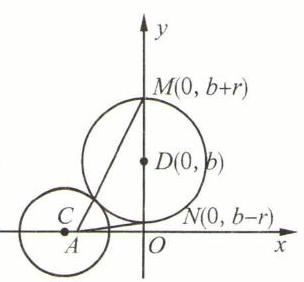
\includegraphics[width=0.2\textwidth]{bodyxb/src/bo_d20aucref24c73anc48g_69_1110_141_304_282_0.jpg}
\end{center}


(第 66 题)

66. 已知圆 $C : {\left( x + 4\right) }^{2} + {y}^{2} = 4$ 和点 $A\left( {-2\sqrt{3},0}\right)$ ,圆 $D$ 的圆心在 $y$ 轴上移动,且恒与圆 $C$ 外切. 设圆 $D$ 与 $y$ 轴交于点 $M,N$ (如图),求证: $\angle {MAN}$ 为定值.

\section*{(四)轨迹}

\section*{【典型题型和解题技巧】}

求动点的轨迹方程, 是解析几何中比较重要的一个内容, 课本已介绍了基本的方法 (姑且称之“基本法”),这里再介绍一些其他较为常用的方法.

1. 转移代入法 (坐标代换法).

转移代入法专门用来求“从动点”[即随已知曲线上的点 (称主动点) 的变化而变化的动点] 的轨迹方程, 其解题步骤是:

(1)设从动点为(x, y),已知曲线上的主动点为 $\left( {{x}_{0},{y}_{0}}\right)$ .

(2)求出用 $x,y$ 表示 ${x}_{0},{y}_{0}$ 的表达式.

(3)将 $\left( {{x}_{0},{y}_{0}}\right)$ 代入已知曲线方程,化简后得动点的轨迹方程.

例 1 已知定点 $A\left( {4,0}\right)$ 和圆 ${x}^{2} + {y}^{2} = 4$ 上的动点 $B$ ,点 $P$ 分 $\vv{AB}$ 之比为 $2 : 1$ (如图 16),求点 $P$ 的轨迹方程.

\begin{center}
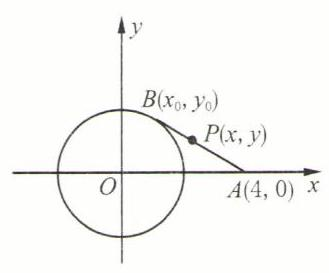
\includegraphics[width=0.2\textwidth]{bodyxb/src/bo_d20aucref24c73anc48g_69_1061_1123_329_273_0.jpg}
\end{center}


(图 16)

解 设动点 $P\left( {x,y}\right)$ 及圆上的点 $B\left( {{x}_{0},{y}_{0}}\right)$ .

$\therefore \left\{  {\begin{array}{l} x = \dfrac{4 + 2{x}_{0}}{1 + 2}, \\  y = \dfrac{2{y}_{0}}{1 + 2}, \end{array}\text{ 于是 }\left\{  \begin{array}{l} {x}_{0} = \dfrac{{3x} - 4}{2}, \\  {y}_{0} = \dfrac{3y}{2}, \end{array}\right. }\right.$

代入圆的方程 ${x}^{2} + {y}^{2} = 4$ ,得 ${\left( \dfrac{{3x} - 4}{2}\right) }^{2} + \dfrac{9}{4}{y}^{2} = 4$ ,

$\therefore$ 点 $P$ 的轨迹方程为 ${\left( x - \dfrac{4}{3}\right) }^{2} + {y}^{2} = \dfrac{16}{9}$ .

2. 几何法.

所谓“几何法”,就是充分利用已知图形的几何性质求动点轨迹方程的方法. 这种方法的优越性在于“化繁为简”.

\begin{center}
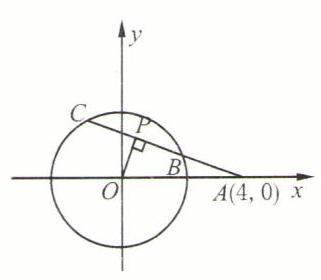
\includegraphics[width=0.2\textwidth]{bodyxb/src/bo_d20aucref24c73anc48g_69_1069_1745_321_280_0.jpg}
\end{center}


(图 17)

例 2 自点 $A\left( {4,0}\right)$ 引圆 $O : {x}^{2} + {y}^{2} = 4$ 的割线 ${ABC}$ (如图 17),求弦 ${BC}$ 中点 $P$ 的轨迹方程.

解法一 连接 ${PO}$ ,则 ${PO} \bot  {PA}$ ,

$\therefore$ 点 $P$ 在以 ${OA}$ 为直径的圆上,即 ${\left( x - 2\right) }^{2} + {y}^{2} = 4$ (在已知圆 $O$ 内的部分).

解法二 连接 ${PO}$ ,则 ${PO} \bot  {PA},\therefore {\left| PO\right| }^{2} + {\left| PA\right| }^{2} = {\left| OA\right| }^{2}$ ,

即 ${x}^{2} + {y}^{2} + {\left( x - 4\right) }^{2} + {y}^{2} = {16}$ ,即 ${x}^{2} + {y}^{2} - {4x} = 0$ (在已知圆 $O$ 内的部分).

注意 也可由 $\dfrac{y}{x} \cdot  \dfrac{y - 0}{x - 4} =  - 1$ 而得.

例 3 已知 $P\left( {4,2}\right)$ 是圆 $C : {x}^{2} + {y}^{2} - {24x} - {28y} - {36} = 0$ 内的一个定点,圆上的动点 $A,B$ 满足 $\angle {APB} = {90}^{ \circ  }$ (如图 18),求弦 ${AB}$ 的中点 $Q$ 的轨迹方程.

解 设动点 $Q$ 为(x, y),圆 $C$ 即为 ${\left( x - {12}\right) }^{2} + {\left( y - {14}\right) }^{2} = {376}$ ,连接 ${CA},{CQ},{PQ}$ ,则 ${CQ} \bot  {AB}$ .

\begin{center}
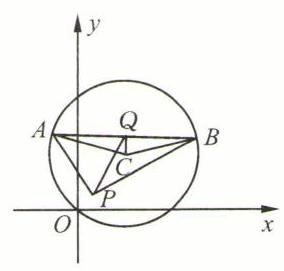
\includegraphics[width=0.2\textwidth]{bodyxb/src/bo_d20aucref24c73anc48g_70_1197_483_284_271_0.jpg}
\end{center}


(图 18)

又 $\because \angle {APB} = {90}^{ \circ  },\therefore \left| {PQ}\right|  = \left| {AQ}\right|$ .

由 ${\left| AQ\right| }^{2} + {\left| CQ\right| }^{2} = {\left| CA\right| }^{2}$ ,得 ${\left| PQ\right| }^{2} + {\left| CQ\right| }^{2} = {376}$ ,

即 ${\left( x - 4\right) }^{2} + {\left( y - 2\right) }^{2} + {\left( x - {12}\right) }^{2} + {\left( y - {14}\right) }^{2} = {376}$ ,

即 ${x}^{2} + {y}^{2} - {16x} - {16y} - 8 = 0$ (该圆位于圆 $C$ 内部),即为点 $Q$ 的轨迹方程.

注意 “几何法”中经常用到的图形性质主要有:

(1)直角三角形:勾股定理,斜边上的中点到三个顶点等距离；

(2)圆:垂径定理,相交弦定理；

(3)相似三角形的有关性质.

\section*{【训练题】}

(A)

67. 已知动圆 $P$ 与圆 ${\left( x + 2\right) }^{2} + {y}^{2} = 4$ 外切,又与直线 $x - 2 = 0$ 相切,则点 $P$ 的轨迹方程为(   )

(A) ${y}^{2} = {12}\left( {x - 1}\right)$ . (B) ${y}^{2} =  - {12}\left( {x - 1}\right)$ .

\begin{center}
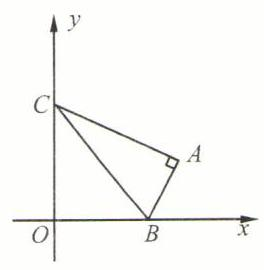
\includegraphics[width=0.2\textwidth]{bodyxb/src/bo_d20aucref24c73anc48g_70_1220_1442_264_270_0.jpg}
\end{center}


(第 68 题)

(C) ${y}^{2} =  - {8x}$ . (D) ${y}^{2} = 6\left( {x - 1}\right)$ .

68. 已知 $\mathrm{{Rt}}\bigtriangleup {ABC}$ 的斜边 ${BC}$ 的两个端点分别在 $x$ 轴、 $y$ 轴正方向上移动,顶点 $A$ 和原点分别在 ${BC}$ 的两侧 (如图),则点 $A$ 的轨迹是 (   )

(A) 圆. (B) 线段.

(C) 射线. (D) 一段圆弧.

\section*{(B)}

69. 用“基本法”解以下各题:

(1)已知 $A\left( {-1,1}\right) ,B\left( {-2,0}\right)$ 是 $\bigtriangleup  {ABC}$ 的两个顶点,且 $\left| {AC}\right|  = \sqrt{2}\left| {BC}\right|$ ,求顶点 $C$ 的轨迹方程;

(2)已知点 $P$ 到定点 $F\left( {-1,0}\right)$ 的距离是点 $P$ 到定直线 $x =  - 4$ 距离的一半,求点 $P$ 的轨迹方程;

( 3 )求与 $x$ 轴和射线 $y =  - \sqrt{3}x\left( {x < 0}\right)$ 都相切的圆的圆心轨迹方程；

(4)过点 $A\left( {2,1}\right)$ 引动直线和 $x$ 轴、 $y$ 轴分别交于 $B,C$ 两点,求线段 ${BC}$ 中点 $P$ 的轨迹方程;

(5)已知 $\bigtriangleup  {ABC}$ 的两个顶点坐标分别是 $B\left( {-5,0}\right)$ 和 $C\left( {5,0}\right)$ ,且 $\angle {ABC} + \angle {ACB} = {135}^{ \circ  }$ , 顶点 $A$ 在 $x$ 轴上方,求顶点 $A$ 的轨迹方程;

(6)求与 $y$ 轴相切且和半圆 ${x}^{2} + {y}^{2} = 4\left( {x \geq  0}\right)$ 内切的动圆的圆心轨迹方程.

70. 用“转移代入法”解以下各题:

(1)已知点 $A$ 在圆 ${x}^{2} + {y}^{2} = {16}$ 上移动, $P\left( {x,y}\right)$ 是连接点 $M\left( {8,0}\right)$ 和点 $A$ 的线段的中点, 求点 $P$ 的轨迹方程;

(2)已知圆 ${x}^{2} + {y}^{2} = 9$ 上的定点 $P\left( {0,3}\right)$ 及动点 $Q$ ,延长弦 ${PQ}$ 至点 $R$ ,使 $\dfrac{PQ}{QR} = \dfrac{1}{3}$ ,求点 $R$ 的轨迹方程;

(3)已知定点 $A\left( {2,0}\right)$ 及圆 ${x}^{2} + {y}^{2} = 1$ 上的动点 $Q,\angle {AOQ}$ 的角平分线交 ${AQ}$ 于点 $P(O$ 为坐标原点),求动点 $P$ 的轨迹方程;

(4)已知点 $A\left( {-1,0}\right)$ 与点 $B\left( {1,0}\right) ,C$ 是圆 ${x}^{2} + {y}^{2} = 1$ 上的动点,连接 ${BC}$ 并延长到点 $D$ , 使 $\left| {CD}\right|  = \left| {BC}\right|$ ,求 ${AC}$ 与 ${OD}$ ( $O$ 为坐标原点) 的交点 $P$ 的轨迹方程.

71. 用“几何法”解以下各题:

(1)已知定点 $A\left( {a,b}\right) \left( {a > 0,b > 0}\right) ,B,C$ 分别是 $x$ 轴、 $y$ 轴上的动点,满足 $\angle {BAC} = {90}^{ \circ  }$ , 且点 $A,O$ 位于 ${BC}$ 的两侧 (如图),求 ${BC}$ 中点 $P$ 的轨迹方程;

\begin{center}
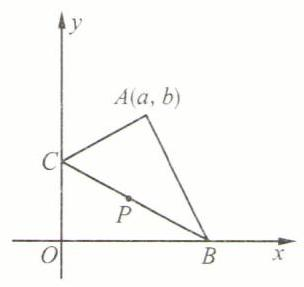
\includegraphics[width=0.2\textwidth]{bodyxb/src/bo_d20aucref24c73anc48g_71_338_1169_304_287_0.jpg}
\end{center}


[第 71(1)题]

\begin{center}
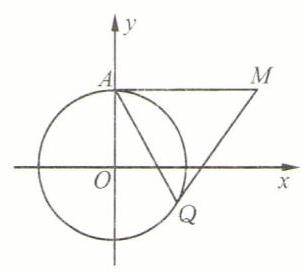
\includegraphics[width=0.2\textwidth]{bodyxb/src/bo_d20aucref24c73anc48g_71_902_1183_302_273_0.jpg}
\end{center}


[第 71(6)题]

(2)一动圆恒与 $y$ 轴相切,且在 $x$ 轴上所截得的弦长为 2,求动圆圆心 $P$ 的轨迹方程；

(3)一动圆被两直线 ${3x} + y = 0,{3x} - y = 0$ 截得的弦长分别为 8 和 4,求动圆圆心 $P$ 的轨迹方程;

(4)自点 $A\left( {-3,2}\right)$ 引圆 ${\left( x - 1\right) }^{2} + {\left( y + 4\right) }^{2} = 9$ 的割线 ${ABC}$ ,求弦 ${BC}$ 的中点 $P$ 的轨迹方程;

(5)已知圆 ${x}^{2} + {y}^{2} = {a}^{2}$ 和定点 $C\left( {c,0}\right) \left( {a > 0,c \neq   \pm  a}\right) ,A,B$ 为圆周上的两个动点,且满足 $\angle {ACB} = {90}^{ \circ  }$ ,求弦 ${AB}$ 的中点 $P$ 的轨迹;

(6)已知定点 $A\left( {0,2}\right)$ 及 $\odot  O : {x}^{2} + {y}^{2} = 4$ ,过点 $A$ 作 ${MA}$ 切 $\odot  O$ 于点 $A$ , $M$ 为切线上的一个动点, ${MQ}$ 切 $\odot  O$ 于点 $Q$ (如图),求 $\bigtriangleup {MAQ}$ 的垂心 $H$ 的轨迹方程.

\section*{三、椭圆}

\section*{(一) 椭圆的基本性质}

\section*{【典型题型和解题技巧】}

1. 椭圆焦点的位置.

椭圆焦点位置的确定十分重要, 它是正确解决与椭圆基本性质有关的问题的前提.

\begin{center}
\begin{tabular}{|c|c|c|c|c|c|}
\hline
焦点的 位置 & 图 形 & 方 程 & 焦 点 & 顶点 & 离心率 \\
\cline{1-6}
焦点在 $x$ 轴上 &  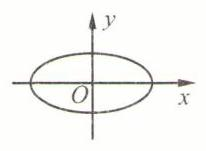
\includegraphics[width=0.2\textwidth]{bodyxb/src/bo_d20aucref24c73anc48g_72_315_761_206_151_0.jpg}  & $\dfrac{{x}^{2}}{{a}^{2}} + \dfrac{{y}^{2}}{{b}^{2}} = 1\left( {a > b > 0}\right)$ & $\left( {\pm c,0}\right) ,c = \sqrt{{a}^{2} - {b}^{2}}$ & $\left( {\pm a,0}\right) ,\left( {0, \pm  b}\right)$ & $e = \dfrac{c}{a}$ \\
\cline{1-6}
焦点在 $y$ 轴上 &  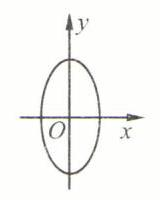
\includegraphics[width=0.2\textwidth]{bodyxb/src/bo_d20aucref24c73anc48g_72_337_968_160_200_0.jpg}  & $\dfrac{{x}^{2}}{{b}^{2}} + \dfrac{{y}^{2}}{{a}^{2}} = 1\left( {a > b > 0}\right)$ & $\left( {0, \pm  c}\right) ,c = \sqrt{{a}^{2} - {b}^{2}}$ & $\left( {\pm b,0}\right) ,\left( {0, \pm  a}\right)$ & $e = \dfrac{c}{a}$ \\
\cline{1-6}
\hline
\end{tabular}
\end{center}

例 1 已知椭圆 $m{x}^{2} + {y}^{2} = 8$ 与 $9{x}^{2} + {25}{y}^{2} = {100}$ 的焦距相等,求实数 $m$ 的值.

解 由 $9{x}^{2} + {25}{y}^{2} = {100}$ ,得 $\dfrac{{x}^{2}}{\dfrac{100}{9}} + \dfrac{{y}^{2}}{4} = 1$ ,故 $a = \dfrac{10}{3},b = 2,c = \sqrt{{a}^{2} - {b}^{2}} = \dfrac{8}{3}$ .

由 $m{x}^{2} + {y}^{2} = 8$ ,得 $\dfrac{{x}^{2}}{\dfrac{8}{m}} + \dfrac{{y}^{2}}{8} = 1$ . 若它的焦点在 $x$ 轴上,则 $\dfrac{8}{m} - 8 = \dfrac{64}{9},\therefore m = \dfrac{9}{17}$ ;

若它的焦点在 $y$ 轴上,则 $8 - \dfrac{8}{m} = \dfrac{64}{9},\therefore m = 9$ .

于是 $m = \dfrac{9}{17}$ 或 $m = 9$ .

2. 利用椭圆的定义解题.

根据椭圆的定义, 有:

椭圆 $\dfrac{{x}^{2}}{{a}^{2}} + \dfrac{{y}^{2}}{{b}^{2}} = 1$ 上的点到焦点的距离与到相应直线 $x =  \pm  \dfrac{{a}^{2}}{c}$ 的距离之比为定值 $e\left( {0 < e = \dfrac{c}{a} < 1}\right)$ .

一些与椭圆的焦半径 (连接椭圆上的点与焦点的线段)、焦点弦 (椭圆过焦点的弦) 等有关的问题,常常可以利用椭圆的定义求解.

例 2 已知点 $P$ 在椭圆 $\dfrac{{x}^{2}}{25} + \dfrac{{y}^{2}}{16} = 1$ 上,且点 $P$ 到椭圆左、右焦点的距离之比为 $1 : 4$ ,求点 $P$ 到两个焦点的距离.

\begin{center}
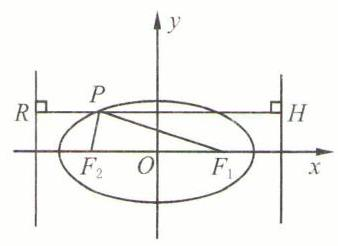
\includegraphics[width=0.2\textwidth]{bodyxb/src/bo_d20aucref24c73anc48g_73_1066_145_338_246_0.jpg}
\end{center}


(图 19)

解 如图 19,不妨设 $\dfrac{\left| P{F}_{2}\right| }{\left| P{F}_{1}\right| } = \dfrac{1}{4}$ ,结合 $\left| {P{F}_{1}}\right|  + \left| {P{F}_{2}}\right|  = {10}$ ,得 $\left| {P{F}_{1}}\right|  = 8,\left| {P{F}_{2}}\right|  = 2.$ 3. 椭圆的弦长.

若直线 $y = {kx} + b$ 和二次曲线 $A{x}^{2} + C{y}^{2} + {Dx} + {Ey} + F = 0$ 相交,所得的弦长可按下面的方法求解:

由两方程中消去 $y$ ,得 $a{x}^{2} + {bx} + c = 0$ ,记 $\Delta  = {b}^{2} - {4ac}$ ,容易证明,弦长 $= \dfrac{\sqrt{\Delta \left( {1 + {k}^{2}}\right) }}{\left| a\right| }$ .

例 3 设直线 $l$ 过点 $P\left( {-1,0}\right)$ ,倾角为 $\dfrac{\pi }{3}$ ,求 $l$ 被椭圆 ${x}^{2} + 2{y}^{2} = 4$ 所截得的弦长.

解 直线 $l$ 的方程为 $y = \sqrt{3}x + \sqrt{3}$ . 代入椭圆方程,得 $7{x}^{2} + {12x} + 2 = 0$ .

$\because \Delta  = {144} - 4 \times  7 \times  2 = {88},\therefore$ 弦长 $= \dfrac{\sqrt{{88}\left( {1 + 3}\right) }}{7} = \dfrac{4\sqrt{22}}{7}$ .

\section*{【训练题】}

\section*{(A)}

72. 若关于 $x,y$ 的方程 ${x}^{2}\sin \alpha  - {y}^{2}\cos \alpha  = 1$ 所表示的曲线是椭圆,则方程

${\left( x + \cos \alpha \right) }^{2} + {\left( y + \sin \alpha \right) }^{2} = 1$ 所表示的圆的圆心在 (   )

(A) 第一象限. (B) 第二象限. (C) 第三象限. (D) 第四象限.

73. 若方程 $\dfrac{{x}^{2}}{{25} - m} + \dfrac{{y}^{2}}{{16} + m} = 1$ 表示焦点在 $y$ 轴上的椭圆,则实数 $m$ 的取值范围是 ( )

(A)(-16,25). (B) $\left( {\dfrac{9}{2},{25}}\right)$ .

(C) $\left( {-{16},\dfrac{9}{2}}\right)$ . (D) $\left( {\dfrac{9}{2}, + \infty }\right)$ .

74. 若圆 ${\left( x - a\right) }^{2} + {y}^{2} = 9$ 与椭圆 $\dfrac{{x}^{2}}{9} + \dfrac{{y}^{2}}{4} = 1$ 有公共点,则实数 $a$ 的取值范围是 (   )

(A) $\left( {-\infty , + \infty }\right)$ . (B) $\left\lbrack  {-6,6}\right\rbrack$ . (C) $\left\lbrack  {-\dfrac{5}{3},\dfrac{5}{3}}\right\rbrack$ . (D) $\varnothing$ .

75. 过椭圆 $\dfrac{{x}^{2}}{{a}^{2}} + \dfrac{{y}^{2}}{{b}^{2}} = 1\left( {a > b > 0}\right)$ 的一个焦点 $F$ 作垂直于长轴的椭圆的弦,则这条弦的长度等于(   )

(A) $\dfrac{{b}^{2}}{2a}$ . (B) $\dfrac{{b}^{2}}{a}$ . (C) $\dfrac{\sqrt{2}{b}^{2}}{a}$ . (D) $\dfrac{2{b}^{2}}{a}$ .

76. 椭圆 $\dfrac{{x}^{2}}{{a}^{2}} + \dfrac{{y}^{2}}{{b}^{2}} = 1$ 的两个焦点和中心将两条直线 $x =  \pm  \dfrac{{a}^{2}}{c}$ (其中 $c = \sqrt{{a}^{2} - {b}^{2}}$ ) 间的距离四等分, 则一焦点与短轴两端点连线的夹角等于 (   )

(A) $\dfrac{\pi }{4}$ . (B) $\dfrac{\pi }{3}$ . (C) $\dfrac{\pi }{2}$ . (D) $\dfrac{2}{3}\pi$ .

77. 若椭圆 $\dfrac{{x}^{2}}{{m}^{2}} + \dfrac{{y}^{2}}{{\left( m - 1\right) }^{2}} = 1$ 的焦点在 $y$ 轴上,则下列结论正确的是 (   )

(A) $0 < m < \dfrac{1}{2}$ . (B) $m < \dfrac{1}{2}$ 且 $m \neq  0$ .

(C) $m > \dfrac{1}{2}$ 且 $m \neq  1$ . (D) $m > 0$ 且 $m \neq  1$ .

78. 已知椭圆 $\dfrac{{x}^{2}}{{a}^{2}} + \dfrac{{y}^{2}}{{b}^{2}} = 1\left( {a > b > 0}\right)$ ,直线 $x =  - \dfrac{{a}^{2}}{c}$ 与直线 $x = \dfrac{{a}^{2}}{c}$ 之间的距离是焦距的 3 倍,则它的离心率是(   )

(A) 3 . (B) $\sqrt{3}$ . (C) $\dfrac{\sqrt{3}}{3}$ . (D) $\dfrac{1}{3}$ .

79. 若 ${F}_{1},{F}_{2}$ 是椭圆 $\dfrac{{x}^{2}}{{a}^{2}} + \dfrac{{y}^{2}}{{b}^{2}} = 1\left( {a > b > 0}\right)$ 的两个焦点, ${AB}$ 是过点 ${F}_{1}$ 的弦,则 $\bigtriangleup  {AB}{F}_{2}$ 的周长是(   )

(A) ${2a}$ . (B) ${4a}$ . (C) ${8a}$ . (D) ${2a} + {2b}$ .

80. 若椭圆的长半轴长、短半轴长、半焦距分别为 $a,b,c$ ,则其焦点 $F\left( {c,0}\right)$ 到直线 $x = \dfrac{{a}^{2}}{c}$ 的距离 $p$ 等于(   )

(A) $\dfrac{{a}^{2}}{c}$ . (B) $\dfrac{{b}^{2}}{c}$ . (C) $\dfrac{{b}^{2}}{a}$ . (D) $\dfrac{{a}^{2}}{b}$ .

81. 已知(0, - 4)是椭圆 ${3k}{x}^{2} + k{y}^{2} = 1$ 的一个焦点,那么实数 $k$ 的值是 ( )

(A) 6 . (B) $\dfrac{1}{6}$ . (C) 24. (D) $\dfrac{1}{24}$ .

82. (1) 若方程 $\dfrac{{x}^{2}}{k - 5} + \dfrac{{y}^{2}}{3 - k} =  - 1$ 表示椭圆,则实数 $k$ 的取值范围是\blkda{};

(2)若方程 ${x}^{2}\sin \alpha  - {y}^{2}\cos \alpha  = 1\left( {0 \leq  \alpha  < {2\pi }}\right)$ 表示焦点在 $y$ 轴上的椭圆,则 $\alpha$ 的取值范围是\blkda{}.

83. (1)若椭圆的长轴长、短轴长、焦距依次成等差数列,则它的离心率 $e =$ \blkda{}；

(2)以椭圆的两个焦点为直径端点的圆交椭圆于四个点,若顺次连接这四个点及两个焦点恰好组成一个正六边形,则椭圆的离心率为\blkda{}；

(3)已知 ${F}_{1},{F}_{2}$ 是椭圆的两个焦点, $P$ 是椭圆上一点, $\bigtriangleup P{F}_{1}{F}_{2}$ 满足 $\angle P{F}_{1}{F}_{2}$ : $\angle P{F}_{2}{F}_{1} : \angle {F}_{1}P{F}_{2} = 1 : 2 : 3$ ,则此椭圆的离心率是\blkda{}.

84. 根据下列条件,写出椭圆的标准方程:

(1) 过点 $P\left( {3,0}\right)$ ,且长轴长是短轴长的 3 倍,\blkda{},

(2)以直线 ${3x} + {4y} - {12} = 0$ 和两轴的交点分别作为顶点和焦点:\blkda{}；

(3)一个焦点把长轴分成长度为 7 和 1 两段:\blkda{}；

(4)长轴长与短轴长之比为 $2 : 1$ ,且 $\dfrac{{a}^{2}}{c} = 4$ :\blkda{}；

(5)长轴在 $x$ 轴上,离心率为 $\dfrac{\sqrt{5}}{3}$ ,且 $\dfrac{{a}^{2}}{c} = 3$ :\blkda{}；

(6)焦点在 $x$ 轴上,其长轴右顶点与右焦点相距为 1,且到直线 $x = \dfrac{{a}^{2}}{c}$ 的距离为 $\dfrac{5}{3}$ :\blkda{}. (B)

85. 若椭圆 $\dfrac{{x}^{2}}{100} + \dfrac{{y}^{2}}{36} = 1$ 上一点 $P$ 到右焦点的距离为 8,则点 $P$ 到它的左焦点的距离是(   )

(A) 14. (B) 12 . (C) 10. (D) 8 .

86. 若 $b < a < 0$ ,则椭圆 $a{x}^{2} + b{y}^{2} + {ab} = 0$ 的焦点坐标是(   )

(A) $\left( {\pm \sqrt{a - b},0}\right)$ . (B) $\left( {0, \pm  \sqrt{a - b}}\right)$ .

(C) $\left( {\pm \sqrt{b - a},0}\right)$ . (D) $\left( {0, \pm  \sqrt{b - a}}\right)$ .

87. 已知椭圆短轴的两顶点为 ${B}_{1},{B}_{2}$ ,过其左焦点 ${F}_{1}$ 作 $x$ 轴的垂线交椭圆于点 $P$ . 若 $\left| {{F}_{1}{B}_{2}}\right|$ 是 $\left| {O{F}_{1}}\right|$ 和 $\left| {{B}_{1}{B}_{2}}\right|$ 的比例中项 $\left( {O\text{ 为中心 }}\right)$ ,则 $\dfrac{\left| P{F}_{1}\right| }{\left| O{B}_{2}\right| } =$ (   )

(A) $\sqrt{2}$ . (B) $\dfrac{\sqrt{2}}{2}$ . (C) $\dfrac{\sqrt{3}}{2}$ . (D) $\dfrac{\sqrt{2}}{3}$ .

88. (1) 已知 $P$ 为椭圆 $\dfrac{{x}^{2}}{25} + \dfrac{{y}^{2}}{9} = 1$ 上的点,且点 $P$ 与两焦点的连线互相垂直,求点 $P$ 的坐标;

( 2 )已知椭圆 $\dfrac{{x}^{2}}{9} + \dfrac{{y}^{2}}{4} = 1$ 上的点 $P$ 到其右焦点的距离是长轴两顶点到右焦点的距离的等差中项,求点 $P$ 的坐标.

89. (1) 中心在原点,两个焦点在 $x$ 轴上的椭圆上有一点 $P\left( {3,y}\right)$ ,若点 $P$ 到两焦点的距离分别为 6.5 和 3.5 , 求此椭圆的标准方程;

(2)已知 $P$ 是椭圆 $\dfrac{{x}^{2}}{45} + \dfrac{{y}^{2}}{20} = 1$ 在第一象限内的点,点 $P$ 与两焦点 ${F}_{1},{F}_{2}$ 的连线互相垂直,求点 $P$ 的横坐标.

90. 已知椭圆 ${x}^{2} + 2{y}^{2} = {12}$ 及 $x$ 轴正半轴上一定点 $A$ ,过点 $A$ 作斜率为 1 的直线,此直线被椭圆截得的弦长为 $\dfrac{4\sqrt{14}}{3}$ ,求点 $A$ 的坐标.

\section*{(二) 椭圆的综合应用}

\section*{【典型题型和解题技巧】}

1. “点差法”解与弦中点有关的题型.

例 1 已知椭圆 $\dfrac{{x}^{2}}{2} + {y}^{2} = 1$ .

(1)求斜率为 2 的平行弦的中点轨迹方程；

(2)过点 $A\left( {2,1}\right)$ 引椭圆的割线,求截得的弦的中点轨迹方程；

( 3 )求过点 $P\left( {\dfrac{1}{2},\dfrac{1}{2}}\right)$ 且被点 $P$ 平分的弦所在的直线方程.

解 设弦的两端点分别为 $M\left( {{x}_{1},{y}_{1}}\right) ,N\left( {{x}_{2},{y}_{2}}\right) ,{MN}$ 的中点为 $R\left( {x,y}\right)$ ,

则 ${x}_{1}^{2} + 2{y}_{1}^{2} = 2,{x}_{2}^{2} + 2{y}_{2}^{2} = 2$ ,

两式相减并除以 $\left( {{x}_{2} - {x}_{1}}\right)$ ,得 ${x}_{2} + {x}_{1} + 2\left( {{y}_{2} + {y}_{1}}\right)  \cdot  \dfrac{{y}_{2} - {y}_{1}}{{x}_{2} - {x}_{1}} = 0$ .

而 ${x}_{1} + {x}_{2} = {2x},{y}_{1} + {y}_{2} = {2y},\therefore x + {2y} \cdot  \dfrac{{y}_{2} - {y}_{1}}{{x}_{2} - {x}_{1}} = 0.\left( *\right)$

(1)将 $\dfrac{{y}_{2} - {y}_{1}}{{x}_{2} - {x}_{1}} = 2$ 代入 $\left( *\right)$ 式,得所求的轨迹方程为 $x + {4y} = 0$ (椭圆内的部分).

(2)将 $\dfrac{{y}_{2} - {y}_{1}}{{x}_{2} - {x}_{1}} = \dfrac{y - 1}{x - 2}$ 代入 $\left( *\right)$ 式,得所求的轨迹方程为 ${x}^{2} + 2{y}^{2} - {2x} - {2y} = 0$ (椭圆内的部分).

(3) 将 ${x}_{1} + {x}_{2} = 1,{y}_{1} + {y}_{2} = 1$ 代入 (*) 式,得 $\dfrac{{y}_{2} - {y}_{1}}{{x}_{2} - {x}_{1}} =  - \dfrac{1}{2}$ ,故所求的直线方程为 ${2x} +$  ${4y} - 3 = 0.$

注意(1)“点差法”的要点是巧代斜率；

(2)与弦的中点有关的问题,主要有三种类型:平行弦的中点轨迹；过定点的弦的中点轨迹;过定点且被定点平分的弦所在的直线方程.

2. 韦达定理的应用.

对于直线 $l$ 与二次曲线相交的一类题型,韦达定理常常为我们提供解题的途径.

例 2 已知直线 $y = x - 1$ 和椭圆 $\dfrac{{x}^{2}}{m} + \dfrac{{y}^{2}}{m - 1} = 1\left( {m > 1}\right)$ 交于点 $A,B$ . 若以 ${AB}$ 为直径的圆过椭圆的左焦点 $F$ (如图 20),求实数 $m$ 的值.

\begin{center}
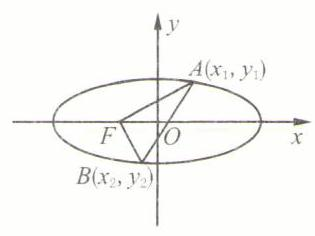
\includegraphics[width=0.2\textwidth]{bodyxb/src/bo_d20aucref24c73anc48g_76_1180_1866_315_236_0.jpg}
\end{center}


(图 20)

解 将 $y = x - 1$ 代入椭圆方程 $\left( {m - 1}\right) {x}^{2} + m{y}^{2} = m\left( {m - 1}\right)$ ,化简得 $\left( {{2m} - 1}\right) {x}^{2} - {2mx} + {2m} - {m}^{2} = 0.\Delta  > 0$ 显然成立.

设点 $A,B$ 的坐标为 $\left( {{x}_{1},{y}_{1}}\right) ,\left( {{x}_{2},{y}_{2}}\right)$ ,则由韦达定理,

得 ${x}_{1} + {x}_{2} = \dfrac{2m}{{2m} - 1},{x}_{1}{x}_{2} = \dfrac{{2m} - {m}^{2}}{{2m} - 1}$ .

由已知易得,左焦点 $F\left( {-1,0}\right)$ 且 $\angle {AFB} = {90}^{ \circ  }$ ,

于是 $\left( {{x}_{1} + 1}\right) \left( {{x}_{2} + 1}\right)  + {y}_{1}{y}_{2} = 0$ ,

即 ${y}_{1}{y}_{2} =  - {x}_{1}{x}_{2} - \left( {{x}_{1} + {x}_{2}}\right)  - 1$ .

又 $A\left( {{x}_{1},{y}_{1}}\right) ,B\left( {{x}_{2},{y}_{2}}\right)$ 在直线 $y = x - 1$ 上,

故 ${y}_{1}{y}_{2} = \left( {{x}_{1} - 1}\right) \left( {{x}_{2} - 1}\right)  = {x}_{1}{x}_{2} - \left( {{x}_{1} + {x}_{2}}\right)  + 1$ ,

于是由上述两式便得 ${x}_{1}{x}_{2} =  - 1$ ,

$\therefore {2m} - {m}^{2} = 1 - {2m}$ ,即 ${m}^{2} - {4m} + 1 = 0$ ,解得 $m = 2 + \sqrt{3}$ .

3. 轨迹.

关于求动点的轨迹,在 “圆” 这一单元,我们已经介绍了 “基本法” “转移代入法” 和 “几何法”,这些方法在椭圆中,还有今后将学到的双曲线和抛物线中仍然常被应用.

这里再介绍两种求动点轨迹的方法.

(1)定义法.

例 3 已知动圆 $M$ 和圆 ${C}_{1} : {\left( x + 1\right) }^{2} + {y}^{2} = {36}$ 内切,并和圆 ${C}_{2} : {\left( x - 1\right) }^{2} + {y}^{2} = 4$ 外切 (如图 21),求动圆圆心 $M$ 的轨迹方程.

解 $\because$ 动圆 $M$ 和圆 ${C}_{1}$ 内切于点 $C$ ,和圆 ${C}_{2}$ 外切于点 $D$ .

\begin{center}
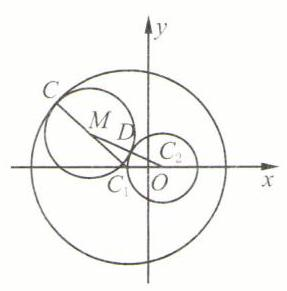
\includegraphics[width=0.2\textwidth]{bodyxb/src/bo_d20aucref24c73anc48g_77_1141_950_287_291_0.jpg}
\end{center}


(图 21)

由 $\left| {MC}\right|  = \left| {MD}\right|$ ,可得

$\left| {M{C}_{1}}\right|  + \left| {M{C}_{2}}\right|  = \left| {M{C}_{1}}\right|  + \left| {MD}\right|  + \left| {D{C}_{2}}\right|  = \left| {C{C}_{1}}\right|  + \left| {D{C}_{2}}\right|  = 6 +$  $2 = 8,$

故点 $M$ 在以 ${C}_{1}\left( {-1,0}\right) ,{C}_{2}\left( {1,0}\right)$ 为两焦点,长轴长为 8 的椭圆上, 此时 $a = 4,c = 1,\therefore b = \sqrt{{a}^{2} - {c}^{2}} = \sqrt{15}$ ,

故点 $M$ 的轨迹方程是 $\dfrac{{x}^{2}}{16} + \dfrac{{y}^{2}}{15} = 1$ .

(2)交轨法.

当动点是两条动直线的交点时,便可以考虑采用“交轨法”.

例 4 已知 ${MN}$ 是椭圆 $\dfrac{{x}^{2}}{{a}^{2}} + \dfrac{{y}^{2}}{{b}^{2}} = 1$ 中垂直于长轴的动弦, $A,B$ 是椭圆的长轴两端点 (如图 22),求直线 ${MA}$ 和 ${NB}$ 的交点 $P$ 的轨迹方程.

解 设 $M\left( {{x}_{0},{y}_{0}}\right)$ ,则 $N\left( {{x}_{0}, - {y}_{0}}\right)$ ,又 $A\left( {-a,0}\right) ,B\left( {a,0}\right)$ ,故得

${l}_{AM} : y = \dfrac{{y}_{0}}{{x}_{0} + a}\left( {x + a}\right) ,{l}_{BN} : y = \dfrac{-{y}_{0}}{{x}_{0} - a}\left( {x - a}\right) .$

\begin{center}
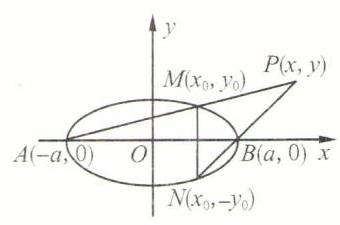
\includegraphics[width=0.2\textwidth]{bodyxb/src/bo_d20aucref24c73anc48g_77_1083_1727_340_225_0.jpg}
\end{center}


(图 22)

两式相乘得 ${y}^{2} = \dfrac{-{y}_{0}^{2}}{{x}_{0}^{2} - {a}^{2}}\left( {{x}^{2} - {a}^{2}}\right)$ .

$\because$ 点 $M\left( {{x}_{0},{y}_{0}}\right)$ 在椭圆上, $\therefore {b}^{2}{x}_{0}^{2} + {a}^{2}{y}_{0}^{2} = {a}^{2}{b}^{2}$ ,

故 ${x}_{0}^{2} - {a}^{2} =  - \dfrac{{a}^{2}}{{b}^{2}}{y}_{0}^{2}$ ,代入上式便得 ${y}^{2} = \dfrac{{b}^{2}}{{a}^{2}}\left( {{x}^{2} - {a}^{2}}\right)$ ,

$\therefore$ 交点 $P$ 的轨迹方程为 $\dfrac{{x}^{2}}{{a}^{2}} - \dfrac{{y}^{2}}{{b}^{2}} = 1\left( {y \neq  0}\right)$ .

\section*{【训练题】}

\section*{(A)}

91. 已知 $F$ 是椭圆 ${b}^{2}{x}^{2} + {a}^{2}{y}^{2} = {a}^{2}{b}^{2}\left( {a > b > 0}\right)$ 的一个焦点, ${PQ}$ 是过其中心的一条弦,记 $c$  $= \sqrt{{a}^{2} - {b}^{2}}$ ,则 $\bigtriangleup  {PQF}$ 面积的最大值是(   )

(A) $\dfrac{1}{2}{ab}$ . (B) ab. (C) ac. (D) ${bc}$ .

92. 若直线 $y = {kx} + 1\left( {k \in  \mathbf{R}}\right)$ 与焦点在 $x$ 轴上的椭圆 $\dfrac{{x}^{2}}{49} + \dfrac{{y}^{2}}{{a}^{2}} = 1$ 总有公共点,则正实数 $a$ 的取值范围是(   )

(A) $0 < a \leq  1$ . (B) $0 < a < 7$ .

(C) $1 \leq  a < 7$ . (D) $1 < a \leq  7$ .

93. 已知 $M$ 为椭圆上一点, ${F}_{1},{F}_{2}$ 是其两个焦点,且 $\angle M{F}_{1}{F}_{2} = {2\alpha },\angle M{F}_{2}{F}_{1} = \alpha \left( {\alpha  \neq  0}\right)$ ,则椭圆的离心率为(   )

(A) $1 - 2\sin \alpha$ . (B) $1 - \sin {2\alpha }$ . (C) $1 - \cos {2\alpha }$ . (D) $2\cos \alpha  - 1$ .

94. 以椭圆的右焦点 ${F}_{2}$ 为圆心作圆,使这圆过椭圆的中心,且交椭圆于点 $M$ . 若直线 $M{F}_{1}$  $\left( {F}_{1}\right.$ 为左焦点)是圆 ${F}_{2}$ 的切线,则椭圆的离心率是 (   )

(A) $\sqrt{3} - 1$ . (B) $2 - \sqrt{3}$ . (C) $\dfrac{\sqrt{2}}{2}$ . (D) $\dfrac{\sqrt{3}}{2}$ .

\section*{(B)}

95. 已知 ${F}_{1}$ 是椭圆 $5{x}^{2} + 9{y}^{2} = {45}$ 的左焦点, $P$ 是此椭圆上的动点, $A\left( {1,1}\right)$ 是一定点,求 $\left| {PA}\right|  + \left| {P{F}_{1}}\right|$ 的最大值.

96. (1) 已知 $P$ 是椭圆 $\dfrac{{x}^{2}}{9} + \dfrac{{y}^{2}}{4} = 1$ 上的点,且 $\angle {F}_{1}P{F}_{2} = {90}^{ \circ  }\left( {{F}_{1},{F}_{2}}\right.$ 是这椭圆的两个焦点), 求 $\bigtriangleup {F}_{1}P{F}_{2}$ 的面积;

( 2 )已知 $P$ 是椭圆 $\dfrac{{x}^{2}}{{a}^{2}} + \dfrac{{y}^{2}}{{b}^{2}} = 1\left( {a > b > 0}\right)$ 上的点, ${F}_{1},{F}_{2}$ 是椭圆的两个焦点,且 $\angle {F}_{1}P{F}_{2}$  $= \theta$ ,求证: $\bigtriangleup {F}_{1}P{F}_{2}$ 的面积为 ${b}^{2}\tan \dfrac{\theta }{2}$ .

97. (1) 求证:椭圆 $\dfrac{{x}^{2}}{{a}^{2}} + \dfrac{{y}^{2}}{{b}^{2}} = 1\left( {a > b > 0}\right)$ 上一点 $P\left( {{x}_{0},{y}_{0}}\right)$ 的两条焦半径 (点 $P$ 和焦点的距离)的长分别为 $a \pm  e{x}_{0}$ ;

(2) $P\left( {x,y}\right)$ 为椭圆 $\dfrac{{x}^{2}}{{a}^{2}} + \dfrac{{y}^{2}}{{b}^{2}} = 1\left( {a > b > 0}\right)$ 上任一点, ${F}_{1},{F}_{2}$ 分别是它的左、右焦点,求证: ${b}^{2} \leq  \left| {P{F}_{1}}\right|  \cdot  \left| {P{F}_{2}}\right|  \leq  {a}^{2};$

(3)求证:椭圆 $\dfrac{{x}^{2}}{{a}^{2}} + \dfrac{{y}^{2}}{{b}^{2}} = 1\left( {a > b > 0}\right)$ 上三点的焦半径成等差数列的充要条件是这三点的横坐标成等差数列.

98. (1)已知直线 $l$ 与椭圆 $4{x}^{2} + 9{y}^{2} = {36}$ 相交于 $A,B$ 两点,弦 ${AB}$ 的中点坐标为(1,1),求直线 $l$ 的方程;

( 2 )已知椭圆 ${x}^{2} + \dfrac{{y}^{2}}{4} = 1$ 和直线 $y = {2x} + m$ 恒有两个不同的公共点,求两公共点连线段的中点轨迹方程;

(3)过点 $A\left( {8,1}\right)$ 引椭圆 $\dfrac{{x}^{2}}{25} + \dfrac{{y}^{2}}{9} = 1$ 的割线交椭圆于 $P,Q$ 两点,求弦 ${PQ}$ 的中点 $M$ 的轨迹方程.

99. (1)已知 $\bigtriangleup  {ABC}$ 的三边 ${AB},{BC},{AC}$ 的长依次成等差数列,且 $\left| {AB}\right|  > \left| {AC}\right|$ ,点 $B,C$ 的坐标分别为 $\left( {-1,0}\right) ,\left( {1,0}\right)$ ,求顶点 $A$ 的轨迹方程;

(2)已知 $B\left( {-8,0}\right) ,C\left( {8,0}\right)$ 是 $\bigtriangleup  {ABC}$ 的两个顶点, ${AB},{AC}$ 边上的中线长之和为 30,分别求此三角形的重心 $G$ 和顶点 $A$ 的轨迹方程;

(3)动圆过定点 $F\left( {0,4}\right)$ ,并和定圆 ${x}^{2} + {\left( y + 4\right) }^{2} = {100}$ 相内切,求动圆圆心 $P$ 的轨迹方程;

(4)过原点的椭圆的一个焦点为 $F\left( {1,0}\right)$ ,其长轴长为 4,求椭圆中心的轨迹方程；

(5)射线 ${OA}$ , ${OB}$ 分别在第一、四象限,且与 $x$ 轴正向成 ${60}^{ \circ  }$ 角, $C$ , $D$ 分别是 ${OA}$ 和 ${OB}$ 上的动点,且满足 $\left| {CD}\right|  = 4\sqrt{3}$ ,求 ${CD}$ 中点 $M$ 的轨迹方程;

(6)求到定点 $\left( {0,\sqrt{7}}\right)$ 和定直线 $y = \dfrac{{16}\sqrt{7}}{7}$ 的距离之比为 $\dfrac{\sqrt{7}}{4}$ 的动点轨迹方程.

100. (1) 已知 $\bigtriangleup {ABC}$ 的三个顶点均在椭圆 $4{x}^{2} + 5{y}^{2} = {80}$ 上,且点 $A$ 是椭圆短轴的一个端点, $\bigtriangleup {ABC}$ 的重心是椭圆的右焦点,试求直线 ${BC}$ 的方程;

(2)已知椭圆中心在原点,长轴在 $x$ 轴上,直线 $x + y = 1$ 被椭圆截得的弦 ${AB}$ 的长为 $2\sqrt{2}$ ,且 ${AB}$ 的中点与椭圆中心连线的斜率为 $\dfrac{\sqrt{2}}{2}$ ,求这个椭圆的方程;

(3)已知椭圆 $\dfrac{{x}^{2}}{{a}^{2}} + \dfrac{{y}^{2}}{{b}^{2}} = 1\left( {a > b > 0}\right)$ 的离心率 $e = \dfrac{\sqrt{2}}{2}$ ,直线 $x$ + $y + 1 = 0$ 与椭圆交于 $P,Q$ 两点,且 ${OP} \bot  {OQ}$ (如图),求这个椭圆的方程;

\begin{center}
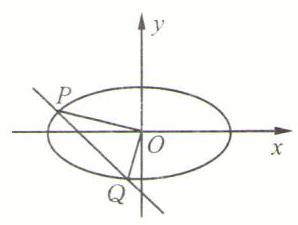
\includegraphics[width=0.2\textwidth]{bodyxb/src/bo_d20aucref24c73anc48g_79_1124_1636_298_225_0.jpg}
\end{center}


[第 100(3)题]

(4)已知中心在原点,一个焦点为 ${F}_{1}\left( {0,\sqrt{50}}\right)$ 的椭圆被直线 $y =$  ${3x} - 2$ 截得的弦的中点横坐标为 $\dfrac{1}{2}$ ,求这个椭圆的方程.

101. (1) 已知动直线 $y = x + t$ 与椭圆 $\dfrac{{x}^{2}}{4} + {y}^{2} = 1$ 交于 $A,B$ 两点,求 $\left| {AB}\right|$ 的最大值;

(2)求点 $P\left( {0,1}\right)$ 到椭圆 $\dfrac{{x}^{2}}{2} + {y}^{2} = 1$ 上点的最大距离；

(3)已知点 $P$ 在圆 ${x}^{2} + {\left( y - 4\right) }^{2} = 1$ 上移动,点 $Q$ 在椭圆 $\dfrac{{x}^{2}}{4} + {y}^{2} = 1$ 上移动,求 $\left| {PQ}\right|$ 的最大值.

102. 已知椭圆 ${x}^{2} + b{y}^{2} = {3a}$ 与直线 $x + y - 1 = 0$ 相交于 $A,B$ 两个不同的点.

(1)当 $a = \dfrac{1}{4}$ 时,求实数 $b$ 的取值范围；

(2)当 $\left| {AB}\right|  = 2\sqrt{2}$ 且 ${AB}$ 的中点 $M$ 与椭圆中心连线的斜率为 $\dfrac{1}{5}$ 时,求椭圆的方程.

103. 已知椭圆 $\dfrac{{x}^{2}}{{a}^{2}} + \dfrac{{y}^{2}}{{b}^{2}} = 1\left( {a > b > 0}\right) ,\dfrac{{a}^{2}}{c} = 1$ ,弦 ${AB}$ 所在直线的倾斜角为 $\dfrac{\pi }{4},M$ 为 ${AB}$ 的中点,直线 ${AB}$ 与 ${OM}$ 的夹角为 $\alpha$ ( $O$ 为原点).

(1)当 $\tan \alpha  = 2$ 时,求椭圆的方程；

(2)当 $2 < \tan \alpha  < 3$ 时,求证: $\dfrac{\sqrt{2}}{3} < b < \dfrac{1}{2}$ .

104. (1) 已知 ${AB}$ 是椭圆 $\dfrac{{x}^{2}}{{a}^{2}} + \dfrac{{y}^{2}}{{b}^{2}} = 1$ 不垂直于坐标轴的任意一条弦, $P$ 是 ${AB}$ 的中点, $O$ 为椭圆的中心,求证: 直线 ${AB},{OP}$ 的斜率之积 ${k}_{AB} \cdot  {k}_{OP} =  - \dfrac{{b}^{2}}{{a}^{2}}$ ;

( 2 )求证: $\dfrac{{x}^{2}}{{a}^{2}} + \dfrac{{y}^{2}}{{b}^{2}} = 1$ 上任一点 $M$ 与短轴两顶点的连线在 $x$ 轴上的截距之积为定值 (如图);

\begin{center}
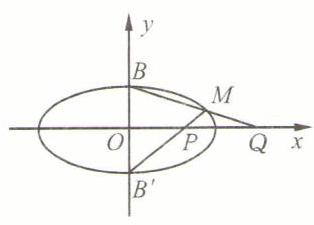
\includegraphics[width=0.2\textwidth]{bodyxb/src/bo_d20aucref24c73anc48g_80_1175_1071_314_225_0.jpg}
\end{center}


[第 104(2)题]

(3)设 $A\left( {{x}_{1},{y}_{1}}\right)$ 为椭圆 ${x}^{2} + 2{y}^{2} = 2$ 上的一点,过点 $A$ 作一条斜率为 $- \dfrac{{x}_{1}}{2{y}_{1}}$ 的直线 $l$ ,又设 $d$ 为原点到直线 $l$ 的距离, ${r}_{1},{r}_{2}$ 分别为点 $A$ 与椭圆两焦点的距离,求证: $\sqrt{{r}_{1} \cdot  {r}_{2}} \cdot  d =$ 常数；

(4)若椭圆 $\dfrac{{x}^{2}}{{a}^{2}} + \dfrac{{y}^{2}}{{b}^{2}} = 1\left( {a > b > 0}\right)$ 上存在一点 $P$ ,使 $\angle {OPA} = {90}^{ \circ  }$ ,其中 $O$ 为原点, $A$ 为右顶点, 求椭圆离心率的取值范围.

105. 设 $P$ 是椭圆 $\dfrac{{x}^{2}}{{a}^{2}} + \dfrac{{y}^{2}}{{b}^{2}} = 1\left( {a > b > 0}\right)$ 上的一点, ${F}_{1},{F}_{2}$ 是椭圆的两个焦点, $e$ 是椭圆的离心率 (如图).

\begin{center}
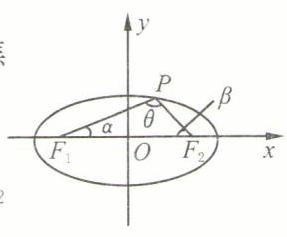
\includegraphics[width=0.2\textwidth]{bodyxb/src/bo_d20aucref24c73anc48g_80_1217_1593_287_237_0.jpg}
\end{center}


(第 105 题)

(1) 若 $\left| {P{F}_{1}}\right|  - \left| {P{F}_{2}}\right|  = {2m}\left( {m > 0}\right)$ ,求证: $\angle {F}_{1}P{F}_{2}$  $= \arccos \dfrac{{m}^{2} + 2{b}^{2} - {a}^{2}}{{a}^{2} - {m}^{2}};$

(2)若 $\angle P{F}_{1}{F}_{2} = \alpha ,\angle P{F}_{2}{F}_{1} = \beta$ ,求证: $\tan \dfrac{\alpha }{2} \cdot  \tan \dfrac{\beta }{2} = \dfrac{1 - e}{1 + e}$ .

106. 已知椭圆的两个焦点分别为 ${F}_{1}\left( {0, - 2\sqrt{2}}\right) ,{F}_{2}\left( {0,2\sqrt{2}}\right)$ ,离心率为 $e = \dfrac{2\sqrt{2}}{3}$ .

\customfootnote{

(1)求这椭圆的方程:

}

(2)是否存在直线 $l$ ,使 $l$ 与此椭圆交于不同的两点 $M$ , $N$ ,且线段 ${MN}$ 恰好被直线 $x =$  $- \dfrac{1}{2}$ 平分? 若存在,求出 $l$ 倾斜角的取值范围.

107. 已知椭圆 $\dfrac{{x}^{2}}{25} + \dfrac{{y}^{2}}{9} = 1$ 上三点 $A\left( {{x}_{1},{y}_{1}}\right) ,B\left( {4,{y}_{2}}\right) ,C\left( {{x}_{3},{y}_{3}}\right)$ 和焦点 $F\left( {4,0}\right)$ 的距离依次成等差数列.

(1) 求 ${x}_{1} + {x}_{3}$ ；

(2)求证:线段 ${AC}$ 的垂直平分线过定点,并求出此定点的坐标.

108. 过原点 $O$ 且倾斜角为 $\theta$ 和 $\pi  - \theta \left( {0 < \theta  < \dfrac{\pi }{2}}\right)$ 的两条直线分别交椭圆 $\dfrac{{x}^{2}}{{a}^{2}} + \dfrac{{y}^{2}}{{b}^{2}} = 1\left( {a > 0,b > 0,a \neq  b}\right)$ 于 $A,C$ 和 $B,D$ 四点 (如图).

\begin{center}
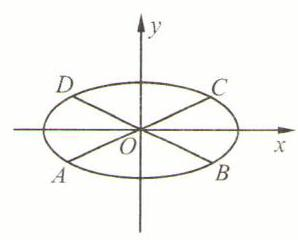
\includegraphics[width=0.2\textwidth]{bodyxb/src/bo_d20aucref24c73anc48g_81_1107_564_298_240_0.jpg}
\end{center}


(第 108 题)

(1)求四边形 ${ABCD}$ 的面积 $S$ (用 $a,b,\theta$ 表示)；

(2)若 $a$ , $b$ 为定值,当 $\theta$ 在 $\left( {0,\dfrac{\pi }{2}}\right)$ 上变化时,求 $S$ 的最大值；

(3)若 $a$ , $b$ 为定值,当 $\theta$ 在 $\left( {0,\dfrac{\pi }{4}}\right\rbrack$ 上变化时,求 $S$ 的最大值.

\section*{四、双曲线}

\section*{(一) 双曲线的基本性质}

\section*{【典型题型和解题技巧】}

1. 双曲线的焦点位置.

先确定双曲线焦点的位置, 再来研究双曲线的基本性质.

\begin{center}
\adjustbox{width=\textwidth}{
\begin{tabular}{|c|c|c|c|c|}
\hline
焦点的位置 & 图 形 & 方 程 焦点 & 顶点 & 离心率 渐近线 \\
\cline{1-5}
焦点在 $x$ 轴上 &  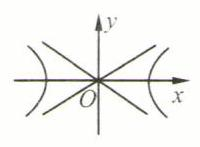
\includegraphics[width=0.2\textwidth]{bodyxb/src/bo_d20aucref24c73anc48g_81_290_1722_200_147_0.jpg}  & $\dfrac{{x}^{2}}{{a}^{2}} - \dfrac{{y}^{2}}{{b}^{2}} = 1\left( {a > 0,b > 0}\right)$  $\left( {\pm c,0}\right) ,\left( {c = \sqrt{{a}^{2} + {b}^{2}}}\right)$ & $\left( {\pm a,0}\right)$ & $e = \dfrac{c}{a}$  $\dfrac{x}{a} \pm  \dfrac{y}{b} = 0$ \\
\cline{1-5}
焦点在 $y$ 轴上 &  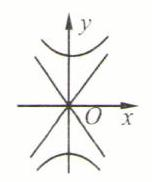
\includegraphics[width=0.2\textwidth]{bodyxb/src/bo_d20aucref24c73anc48g_81_314_1946_152_182_0.jpg}  & $\dfrac{{y}^{2}}{{a}^{2}} - \dfrac{{x}^{2}}{{b}^{2}} = 1\left( {a > 0,b > 0}\right)$  $\left( {0, \pm  c}\right) ,\left( {c = \sqrt{{a}^{2} + {b}^{2}}}\right)$ & $\left( {0, \pm  a}\right)$ & $e = \dfrac{c}{a}$  $\dfrac{y}{a} \pm  \dfrac{x}{b} = 0$ \\
\cline{1-5}
\hline
\end{tabular}
}
\end{center}

例 1 已知双曲线的渐近线方程是 $x \pm  {2y} = 0$ ,求双曲线的离心率.

解 若双曲线的焦点在 $x$ 轴上,则它的方程是 $\dfrac{{x}^{2}}{{a}^{2}} - \dfrac{{y}^{2}}{{b}^{2}} = 1$ ,渐近线方程是 $\dfrac{x}{a} \pm  \dfrac{y}{b} = 0$ ,将已知渐近线方程变形为 $\dfrac{x}{2} \pm  \dfrac{y}{1} = 0,\therefore $ 可设 $a = {2k},b = k$ ,则 $c = \sqrt{5}k,e = \dfrac{c}{a} = \dfrac{\sqrt{5}}{2}$ .

若双曲线的焦点在 $y$ 轴上,则它的方程是 $- \dfrac{{x}^{2}}{{b}^{2}} + \dfrac{{y}^{2}}{{a}^{2}} = 1$ ,渐近线方程是 $\dfrac{x}{b} \pm  \dfrac{y}{a} = 0$ ,将已知渐近线方程变形为 $\pm  \dfrac{x}{2} + \dfrac{y}{1} = 0,\therefore $ 可设 $a = k,b = {2k}$ ,则 $c = \sqrt{5}k,e = \dfrac{c}{a} = \sqrt{5}$ .

由上可知,双曲线的离心率是 $\dfrac{\sqrt{5}}{2}$ 或 $\sqrt{5}$ .

2. 已知离心率或渐近线,求双曲线的方程.

例 2 已知双曲线 $\dfrac{{x}^{2}}{{a}^{2}} - \dfrac{{y}^{2}}{{b}^{2}} = 1$ 的离心率 $e = \dfrac{5}{4}$ ,虚半轴长为 2,求双曲线的方程.

解 $\because e = \dfrac{c}{a} = \dfrac{5}{4}$ ,可令 $a = {4k},c = {5k}$ ,则 ${b}^{2} = {c}^{2} - {a}^{2} = 9{k}^{2} = 4,\therefore {k}^{2} = \dfrac{4}{9}$ .

于是 ${a}^{2} = \dfrac{64}{9},{c}^{2} = \dfrac{100}{9}$ ,故双曲线的方程为 $\dfrac{9{x}^{2}}{64} - \dfrac{{y}^{2}}{4} = 1$ .

注意 对 $\dfrac{c}{a} = \dfrac{5}{4}$ ,不可错误地以为必有 $c = 5,a = 4$ ,它只是表明 $c,a$ 之比为 $\dfrac{5}{4}$ .

例 3 求过点(-1,3),且和双曲线 $\dfrac{{x}^{2}}{4} - \dfrac{{y}^{2}}{9} = 1$ 有共同渐近线的双曲线的方程.

解 可设双曲线的方程为 $\dfrac{{x}^{2}}{4} - \dfrac{{y}^{2}}{9} = \lambda \left( {\lambda  \neq  0}\right)$ ,将(-1,3)代入,得 $\lambda  =  - \dfrac{3}{4}$ .

代入,即得双曲线的方程为 $\dfrac{4{y}^{2}}{27} - \dfrac{{x}^{2}}{3} = 1$ .

注意 和双曲线 $\dfrac{{x}^{2}}{{a}^{2}} - \dfrac{{y}^{2}}{{b}^{2}} = 1$ 有共同渐近线的双曲线可设为 $\dfrac{{x}^{2}}{{a}^{2}} - \dfrac{{y}^{2}}{{b}^{2}} = \lambda \left( {\lambda  \neq  0}\right)$ .

若求得 $\lambda  > 0$ ,则双曲线焦点在 $x$ 轴上; 若求得 $\lambda  < 0$ ,则双曲线的焦点在 $y$ 轴上.

\section*{【训练题】}

\section*{(A)}

109. 当 ${ab} < 0$ 时,方程 $a{x}^{2} - a{y}^{2} = b$ 所表示的曲线是(   )

(A) 焦点在 $x$ 轴上的椭圆. (B) 焦点在 $x$ 轴上的双曲线.

(C) 焦点在 $y$ 轴上的椭圆. (D) 焦点在 $y$ 轴上的双曲线.

110. 已知焦点在 $y$ 轴上的双曲线 $k{x}^{2} - {2k}{y}^{2} = 4$ 的实半轴的平方等于半焦距,则实数 $k$ 的值等于(   )

(A) $\dfrac{3}{2}$ . (B) $- \dfrac{2}{3}$ . (C) $- \dfrac{3}{2}$ . (D) $\dfrac{2}{3}$ .

111. 双曲线与其共轭双曲线有相同的(   )

(A) 顶点. (B) 焦点. (C) 实半轴长. (D) 渐近线.

112. 中心在原点,一个焦点为(3,0),一条渐近线方程为 ${2x} - {3y} = 0$ 的双曲线方程为(   )

(A) $\dfrac{55}{36}{x}^{2} - \dfrac{1}{54}{y}^{2} = 1$ . (B) $\dfrac{5}{54}{x}^{2} - \dfrac{51}{36}{y}^{2} = 1$ .

(C) $\dfrac{13}{81}{x}^{2} - \dfrac{13}{36}{y}^{2} = 1$ . (D) $\dfrac{13}{36}{x}^{2} - \dfrac{13}{81}{y}^{2} = 1$ .

113. 过点(2, - 2)且与双曲线 ${x}^{2} - 2{y}^{2} = 2$ 有公共渐近线的双曲线方程是(   )

(A) $- \dfrac{{x}^{2}}{4} + \dfrac{{y}^{2}}{2} = 1$ . (B) $\dfrac{{x}^{2}}{4} - \dfrac{{y}^{2}}{2} = 1$ .

(C) $- \dfrac{{x}^{2}}{2} + \dfrac{{y}^{2}}{4} = 1$ . (D) $\dfrac{{x}^{2}}{2} - \dfrac{{y}^{2}}{4} = 1$ .

114. 已知双曲线的半焦距为 $c$ ,直线 $x = \dfrac{{a}^{2}}{c}$ 与直线 $x =  - \dfrac{{a}^{2}}{c}$ 之间的距离为 $d$ ,且 $c = d$ ,则双曲线的离心率等于(   )

(A) $\sqrt{3}$ . (B) $\sqrt{2}$ . (C) 3. (D) 2 .

115. 当 $8 < k < {17}$ 时,曲线 $\dfrac{{x}^{2}}{{17} - k} + \dfrac{{y}^{2}}{8 - k} = 1$ 与 $\dfrac{{x}^{2}}{8} + \dfrac{{y}^{2}}{17} = 1$ 有相同的(   )

(A) 焦距. (B) 渐近线. (C) 焦点. (D) 离心率.

116. 已知 $E,F$ 分别是离心率为 $\dfrac{\sqrt{5} + 1}{2}$ 的双曲线 $\dfrac{{x}^{2}}{{a}^{2}} - \dfrac{{y}^{2}}{{b}^{2}} = 1\left( {a > 0,b > 0}\right)$ 的左顶点与右焦点, 点 $M\left( {0,b}\right)$ ,则 $\angle {EMF}$ 等于(   )

(A) ${45}^{ \circ  }$ . (B) ${60}^{ \circ  }$ . (C) ${90}^{ \circ  }$ . (D) ${120}^{ \circ  }$ .

117. 根据下列条件,写出双曲线方程:

(1)以 $y =  \pm  \dfrac{1}{2}x$ 为渐近线,且焦点在坐标轴上,焦距为 10:\blkda{}；

(2)与椭圆 ${x}^{2} + 4{y}^{2} = {64}$ 有共同焦点,且一条渐近线为 $x + \sqrt{3}y = 0$ :\blkda{}；

(3)以 ${2x} \pm  {3y} = 0$ 为渐近线,且经过点(1,2):\blkda{}.

118. (1)若方程 ${x}^{2}\sin \theta  + {y}^{2}\cos \theta  = 1$ 表示双曲线,则 $\theta$ 的取值范围是\blkda{}；

(2)若 $\dfrac{{x}^{2}}{\left| m\right|  - 2} + \dfrac{{y}^{2}}{5 - m} = 1$ 表示双曲线,则实数 $m$ 的取值范围是\blkda{}；

(3)若方程 $\dfrac{{x}^{2}}{a - m} + \dfrac{{y}^{2}}{b - m} = 1\left( {a > b > 0}\right)$ 表示双曲线,则实数 $m$ 的取值范围是\blkda{}, 焦点坐标是\blkda{}；

(4) 曲线 $C$ 的方程为 ${k}^{2}{x}^{2} + \left( {{k}^{2} - 9}\right) {y}^{2} = {k}^{2}\left( {{k}^{2} - 9}\right)$ ,则:

当\blkda{}时, $C$ 表示直线,

当\blkda{}时, $C$ 表示椭圆,

当\blkda{}时, $C$ 表示双曲线.

119. (1) 双曲线 $\dfrac{{x}^{2}}{4} - \dfrac{{y}^{2}}{8} = 1$ 的两渐近线的夹角等于\blkda{}；

(2)若双曲线的离心率为 2,则其共轭双曲线的离心率为\blkda{}；

(3)已知双曲线 $k{x}^{2} - {2k}{y}^{2} + 1 = 0$ 的一个焦点为(-4,0),则实数 $k =$ \blkda{}；

(4)已知双曲线的渐近线方程为 ${3x} \pm  {4y} = 0$ ,则其离心率为\blkda{}.

\section*{(B)}

120. 若方程 $\dfrac{{x}^{2}}{2 - m} + \dfrac{{y}^{2}}{\left| m\right|  - 3} = 1$ 表示双曲线,则实数 $m$ 的取值范围是 (   )

(A) $- 3 < m < 2$ 或 $m > 3$ . (B) $m <  - 3$ 或 $m > 3$ .

(C) $- 2 < m < 3$ . (D) $- 3 < m < 3$ 或 $m > 3$ .

121. 已知双曲线的中心在原点,焦点在 $y$ 轴上. 且一条渐近线方程为 $y = \dfrac{12}{5}x$ ,实半轴的平方与半焦距之比为 $\dfrac{144}{13}$ ,则双曲线的方程是 (   )

(A) $- \dfrac{{x}^{2}}{144} + \dfrac{{y}^{2}}{25} = 1$ . (B) $\dfrac{{x}^{2}}{25} - \dfrac{{y}^{2}}{144} = 1$ .

(C) $\dfrac{{x}^{2}}{144} - \dfrac{{y}^{2}}{25} = 1$ . (D) $- \dfrac{{x}^{2}}{25} + \dfrac{{y}^{2}}{144} = 1$ .

122. 已知双曲线 $\dfrac{{x}^{2}}{64} - \dfrac{{y}^{2}}{36} = 1$ 上的点 $P$ 到右焦点的距离为 14,则点 $P$ 到左焦点的距离为(   )

(A) 22. (B) 30. (C) 26. (D) 28.

123. 双曲线 $\dfrac{{x}^{2}}{16} - \dfrac{{y}^{2}}{25} = 1$ 的两条渐近线的夹角是(   )

(A) $\arctan \dfrac{5}{4}$ . (B) $\pi  - \arctan \dfrac{5}{4}$ . (C) $2\arctan \dfrac{5}{4}$ . (D) arctan $\dfrac{40}{9}$ .

124. (1) 已知 $\lg \left( {x - 2}\right) ,\lg {2y},\lg {16x}$ 依次成等差数列,求点 $M\left( {x,y}\right)$ 的轨迹方程;

(2)试求以椭圆 $\dfrac{{x}^{2}}{169} + \dfrac{{y}^{2}}{144} = 1$ 的右焦点为圆心,且与双曲线 $\dfrac{{x}^{2}}{9} - \dfrac{{y}^{2}}{16} = 1$ 的渐近线相切的圆的方程;

(3)以双曲线 ${12}{x}^{2} - 4{y}^{2} = 3$ 的焦点为焦点作椭圆,使此椭圆与直线 $x - y + 3 = 0$ 有公共点, 且使此椭圆的长轴长最短, 求这个椭圆的方程.

125. (1) 求过双曲线 $4{x}^{2} - {12}{y}^{2} - 3 = 0$ 的左焦点 $F$ ,且与直线 $y = {2x}$ 的夹角为 $\dfrac{\pi }{4}$ 的直线方程;

(2)求直线 ${3x} - y + 3 = 0$ 被曲线 $4{x}^{2} - {y}^{2} - 4 = 0$ 所截得的线段长；

(3)过双曲线 $\dfrac{{x}^{2}}{9} - \dfrac{{y}^{2}}{16} = 1$ 的右焦点 $F$ 作倾斜角为 $\dfrac{\pi }{4}$ 的弦 ${AB}$ ,求弦 ${AB}$ 的长及 ${AB}$ 的中点 $M$ 到右焦点 $F$ 的距离.

\section*{(二) 双曲线的综合应用}

\section*{【典型题型和解题技巧】}

1. 利用双曲线的定义解题.

例 1 若动圆过定点 $A\left( {-3,0}\right)$ ,且和定圆 ${\left( x - 3\right) }^{2} + {y}^{2} = 4$ 外切,求动圆圆心 $P$ 的轨迹方程.

解 如图 23,设动圆 $P$ 和定圆外切于点 $N$ ,则 $\left| {PB}\right|  - \left| {PA}\right|  =$  $\left| {PB}\right|  - \left| {PN}\right|  = \left| {BN}\right|  = 2,$

\begin{center}
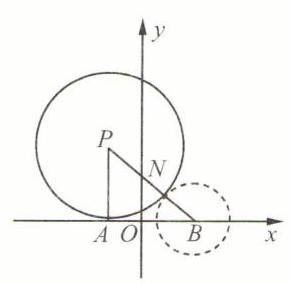
\includegraphics[width=0.2\textwidth]{bodyxb/src/bo_d20aucref24c73anc48g_85_1142_539_290_284_0.jpg}
\end{center}


(图 23)

$\therefore$ 点 $P$ 的轨迹是以 $A,B$ 为焦点,实半轴长为 1 的双曲线的左支, 其方程为 ${x}^{2} - \dfrac{{y}^{2}}{8} = 1\left( {x < 0}\right)$ .

例 2 点 $P$ 是双曲线 $\dfrac{{x}^{2}}{4} - \dfrac{{y}^{2}}{12} = 1$ 右支上任意一点, ${F}_{1},{F}_{2}$ 分别为左、右焦点,设 $\angle P{F}_{1}{F}_{2} = \alpha ,\angle P{F}_{2}{F}_{1} = \beta$ (如图 24),求证: $3\tan \dfrac{\alpha }{2} = \tan \dfrac{\beta }{2}$ .

简证一 在 $\bigtriangleup P{F}_{1}{F}_{2}$ 中,利用正弦定理及分比定理,得 $\dfrac{\left| P{F}_{1}\right| }{\sin \beta } = \dfrac{\left| P{F}_{2}\right| }{\sin \alpha } = \dfrac{\left| {F}_{1}{F}_{2}\right| }{\sin \left( {\alpha  + \beta }\right) } =$  $\dfrac{\left| {P{F}_{1}}\right|  - \left| {P{F}_{2}}\right| }{\sin \beta  - \sin \alpha },\therefore \dfrac{8}{2\sin \dfrac{\alpha  + \beta }{2}\cos \dfrac{\alpha  + \beta }{2}} = \dfrac{4}{2\cos \dfrac{\alpha  + \beta }{2}\sin \dfrac{\beta  - \alpha }{2}}$ ,即 $2\sin \dfrac{\beta  - \alpha }{2} = \sin \dfrac{\alpha  + \beta }{2},$

展开并化简,得 $3\sin \dfrac{\alpha }{2}\cos \dfrac{\beta }{2} = \sin \dfrac{\beta }{2}\cos \dfrac{\alpha }{2}.\therefore 3\tan \dfrac{\alpha }{2} = \tan \dfrac{\beta }{2}$ .

\begin{center}
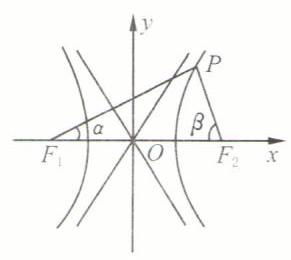
\includegraphics[width=0.2\textwidth]{bodyxb/src/bo_d20aucref24c73anc48g_85_352_1355_291_260_0.jpg}
\end{center}


(图 24)

\begin{center}
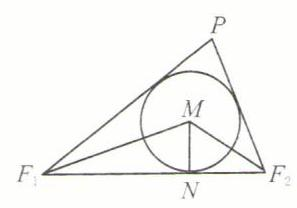
\includegraphics[width=0.2\textwidth]{bodyxb/src/bo_d20aucref24c73anc48g_85_902_1411_297_208_0.jpg}
\end{center}


(图 25)

简证二 如图 25,设 $M$ 是 $\bigtriangleup P{F}_{1}{F}_{2}$ 的内心,连接 $M{F}_{1},M{F}_{2}$ ,并作 ${MN} \bot  {F}_{1}{F}_{2}$ 于点 $N$ ,

则 $\tan \dfrac{\alpha }{2} = \dfrac{\left| MN\right| }{\left| {F}_{1}N\right| },\tan \dfrac{\beta }{2} = \dfrac{\left| MN\right| }{\left| {F}_{2}N\right| }$ .

欲证原等式成立,只需证 $\left| {{F}_{1}N}\right|  = 3\left| {{F}_{2}N}\right|$ ,(   )

而 $\left| {{F}_{1}N}\right|  = \dfrac{\left| {{F}_{1}{F}_{2}}\right|  + \left| {P{F}_{1}}\right|  - \left| {P{F}_{2}}\right| }{2} = \dfrac{8 + 4}{2} = 6$ ,

$\left| {{F}_{2}N}\right|  = \dfrac{\left| {{F}_{1}{F}_{2}}\right|  + \left| {P{F}_{2}}\right|  - \left| {P{F}_{1}}\right| }{2} = \dfrac{8 - 4}{2} = 2.$

故 $\left( *\right)$ 式成立,则原等式成立.

注意 在圆锥曲线中,过焦点的半径或弦称为焦半径或焦点弦. 对于和焦半径或焦点弦有关的问题, 通常用以下三种方法可获解:

(1)利用圆锥曲线的定义；

(2)运用圆锥曲线的光学性质.

本例的两种证法都利用了圆锥曲线的定义, 其中证法二还综合运用了图形的几何性质, 因而显得更简捷.

2. 韦达定理的应用.

例 3 已知直线 $l$ 和双曲线 $\dfrac{{x}^{2}}{{a}^{2}} - \dfrac{{y}^{2}}{{b}^{2}} = 1\left( {a > 0,b > 0}\right)$ 及其渐近线依次交于 $A,B,C,D$ 四点 (如图 26),求证: $\left| {AB}\right|  = \left| {CD}\right|$ .

证明 若直线 $l$ 和 $x$ 轴垂直,结论显然成立.

\begin{center}
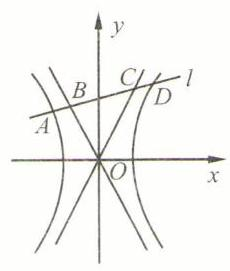
\includegraphics[width=0.2\textwidth]{bodyxb/src/bo_d20aucref24c73anc48g_86_1234_699_230_271_0.jpg}
\end{center}


(图 26)

若直线 $l$ 不与 $x$ 轴垂直,则可设 $l$ 的方程为 $y = {kx} + m$ ,代入双曲线方程 ${b}^{2}{x}^{2} - {a}^{2}{y}^{2} - {a}^{2}{b}^{2} = 0$ ,

整理得 $\left( {{b}^{2} - {a}^{2}{k}^{2}}\right) {x}^{2} - 2{a}^{2}{kmx} - {a}^{2}\left( {{m}^{2} + {b}^{2}}\right)  = 0$ .

设 $A\left( {{x}_{1},{y}_{1}}\right) ,D\left( {{x}_{2},{y}_{2}}\right)$ ,则 ${x}_{1} + {x}_{2} = \dfrac{2{a}^{2}{km}}{{b}^{2} - {a}^{2}{k}^{2}}$ .

再将 $y = {kx} + m$ 代入双曲线的渐近线方程,得 ${b}^{2}{x}^{2} - {a}^{2}{y}^{2} = 0$ ,

并整理得 $\left( {{b}^{2} - {a}^{2}{k}^{2}}\right) {x}^{2} - 2{a}^{2}{kmx} - {a}^{2}{m}^{2} = 0$ .

设 $B\left( {{x}_{3},{y}_{3}}\right) ,C\left( {{x}_{4},{y}_{4}}\right)$ ,则 ${x}_{3} + {x}_{4} = \dfrac{2{a}^{2}{km}}{{b}^{2} - {a}^{2}{k}^{2}}$ .

$\therefore {x}_{1} + {x}_{2} = {x}_{3} + {x}_{4}$ .

这说明线段 ${AD}$ 的中点和线段 ${BC}$ 的中点重合,故 $\left| {AB}\right|  = \left| {CD}\right|$ .

\section*{【训练题】}

\section*{(A)}

126. 过双曲线的一个焦点 ${F}_{2}$ 作垂直于实轴的弦 ${PQ},{F}_{1}$ 是另一焦点. 若 $\angle P{F}_{1}Q = \dfrac{\pi }{2}$ ,则双曲线的离心率是(   )

(A) $\sqrt{2} - 1$ . (B) $\sqrt{2}$ .

(C) $\sqrt{2} + 1$ . (D) $\sqrt{2} + 2$ .

127. 直线 $y = {kx} + 2$ 与双曲线 ${x}^{2} - {y}^{2} = 6$ 的右支交于两个不同的点,则实数 $k$ 的取值范围是(   )

(A) $\left( {-\dfrac{\sqrt{15}}{3},\dfrac{\sqrt{15}}{3}}\right)$ . (B) $\left( {0,\dfrac{\sqrt{15}}{8}}\right)$ .

(C) $\left( {-\dfrac{\sqrt{15}}{3},0}\right)$ . (D) $\left( {-\dfrac{\sqrt{15}}{3}, - 1}\right)$ .

128. 直线 $y = \dfrac{1}{3}\left( {x - \dfrac{7}{2}}\right)$ 与双曲线 $\dfrac{{x}^{2}}{9} - {y}^{2} = 1$ 的公共点个数是 (   )

(A) 0 . (B) 1 . (C) 2 . (D) 4.

129. 双曲线 $\dfrac{{x}^{2}}{{a}^{2}} - \dfrac{{y}^{2}}{{b}^{2}} = 1$ 的渐近线与实轴所夹的锐角为 $\theta$ ,则过焦点且平行于虚轴的弦长等于(   )

(A) ${2a}\cot \theta$ . (B) ${2b}\cot \theta$ . (C) ${2a}\tan \theta$ . (D) ${2b}\tan \theta$ .

130. 和定点 $A\left( {5,0}\right)$ 及定直线 $l : x = \dfrac{16}{5}$ 的距离之比是 $5 : 4$ 的点的轨迹方程是 (   )

(A) $\dfrac{{x}^{2}}{16} + \dfrac{{y}^{2}}{9} = 1$ . (B) $\dfrac{{x}^{2}}{9} - \dfrac{{y}^{2}}{16} = 1$ . (C) $\dfrac{{x}^{2}}{16} - \dfrac{{y}^{2}}{9} = 1$ . (D) $- \dfrac{{x}^{2}}{16} + \dfrac{{y}^{2}}{9} = 1$ .

131. 与两圆 ${x}^{2} + {y}^{2} = 1$ 和 ${x}^{2} + {y}^{2} - {8x} + 7 = 0$ 都相切的圆的圆心轨迹是 (   )

(A) 两个椭圆. (B) 两条双曲线.

(C)一条双曲线和一条直线去掉三个点. (D)一个椭圆与一条双曲线.

132. 已知双曲线 ${x}^{2} - {y}^{2} = 1$ 的左焦点为 $F$ ,点 $P$ 为双曲线在第三象限内的任意一点,且直线 ${PF}$ 不垂直于 $x$ 轴,则斜率 $k$ 的取值范围是 ( )

(A) $k \leq  0$ 或 $k \geq  1$ . (B) $k < 0$ 或 $k > 1$ .

(C) $k \leq   - 1$ 或 $k \geq  1$ . (D) $k <  - 1$ 或 $k > 1$ .

133. 方程 $y = \sqrt{\left| 1 - {x}^{2}\right| }$ 表示的曲线为(   )

\begin{center}
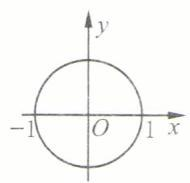
\includegraphics[width=0.2\textwidth]{bodyxb/src/bo_d20aucref24c73anc48g_87_312_1176_190_183_0.jpg}
\end{center}


(A)

\begin{center}
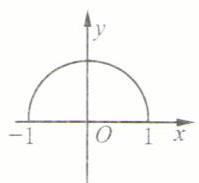
\includegraphics[width=0.2\textwidth]{bodyxb/src/bo_d20aucref24c73anc48g_87_553_1176_199_183_0.jpg}
\end{center}


(B)

\begin{center}
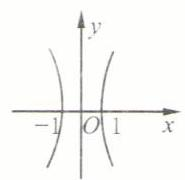
\includegraphics[width=0.2\textwidth]{bodyxb/src/bo_d20aucref24c73anc48g_87_806_1179_185_180_0.jpg}
\end{center}


(C)

\begin{center}
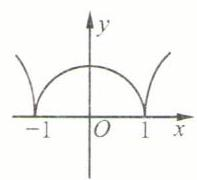
\includegraphics[width=0.2\textwidth]{bodyxb/src/bo_d20aucref24c73anc48g_87_1045_1180_197_180_0.jpg}
\end{center}


(D)

134. 已知 $m,n$ 为两个不相等的非零实数,则方程 ${mx} - y + n = 0$ 与 $n{x}^{2} + m{y}^{2} = {mn}$ 所表示的曲线大致是(   )

\begin{center}
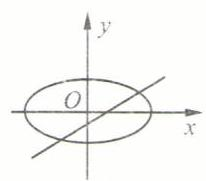
\includegraphics[width=0.2\textwidth]{bodyxb/src/bo_d20aucref24c73anc48g_87_307_1525_206_181_0.jpg}
\end{center}


(A)

\begin{center}
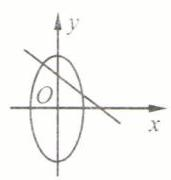
\includegraphics[width=0.2\textwidth]{bodyxb/src/bo_d20aucref24c73anc48g_87_579_1529_171_180_0.jpg}
\end{center}


(B)

\begin{center}
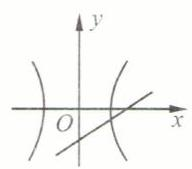
\includegraphics[width=0.2\textwidth]{bodyxb/src/bo_d20aucref24c73anc48g_87_813_1534_192_169_0.jpg}
\end{center}


(C)

\begin{center}
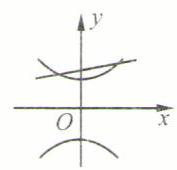
\includegraphics[width=0.2\textwidth]{bodyxb/src/bo_d20aucref24c73anc48g_87_1066_1536_177_170_0.jpg}
\end{center}


(D)

135. 若椭圆 $\dfrac{{x}^{2}}{m} + \dfrac{{y}^{2}}{n} = 1\left( {m > n > 0}\right)$ 和双曲线 $\dfrac{{x}^{2}}{a} - \dfrac{{y}^{2}}{b} = 1\left( {a > 0,b > 0}\right)$ 有相同的焦点 ${F}_{1},{F}_{2}$ , $P$ 是两曲线的一个公共点,则 $\left| {P{F}_{1}}\right|  \cdot  \left| {P{F}_{2}}\right|$ 的值是 (   )

(A) $m - a$ . (B) $\dfrac{1}{2}\left( {m - a}\right)$ . (C) ${m}^{2} - {a}^{2}$ . (D) $\sqrt{m} - \sqrt{a}$ .

136. 若曲线 ${x}^{2} - {y}^{2} = {a}^{2}$ 与曲线 ${\left( x - 1\right) }^{2} + {y}^{2} = 1$ 恰好有三个不同的公共点,则实数 $a$ 的值只能是(   )

(A) $a = 0$ . (B) $a =  \pm  1$ . (C) $0 < \left| a\right|  < 1$ . (D) $\left| a\right|  > 1$ .

137. 已知双曲线 $\dfrac{{x}^{2}}{{a}^{2}} - \dfrac{{y}^{2}}{{b}^{2}} = 1\left( {a > 0,b > 0}\right)$ ,直线 $x = \dfrac{{a}^{2}}{c}$ 与一条渐近线交于点 $P,F$ 是右焦点. (1)求证:直线 ${PF}$ 与这条渐近线垂直；(2)求 $\left| {PF}\right|$ .

138. 已知 $P$ 为双曲线 $3{x}^{2} - 5{y}^{2} = {15}$ 上的一点, ${F}_{1},{F}_{2}$ 为其两个焦点,且 ${S}_{\bigtriangleup {F}_{1}P{F}_{2}} = 3\sqrt{3}$ ,求 $\angle {F}_{1}P{F}_{2}$ 的大小.

* 139. 已知双曲线 $\dfrac{{x}^{2}}{{a}^{2}} - \dfrac{{y}^{2}}{{b}^{2}} = 1\left( {a > 0,b > 0}\right)$ 的离心率 $e > 1 + \sqrt{2}$ ,左、右焦点分别为 ${F}_{1},{F}_{2}$ ,直线 $l$ 为 $x =  - \dfrac{{a}^{2}}{c}$ (如图),能否在双曲线的左半支上找到一点 $P$ ,使 $\left| {P{F}_{1}}\right|$ 是点 $P$ 到 $l$ 的距离 $d$ 与 $\left| {P{F}_{2}}\right|$ 的等比中项?

\begin{center}
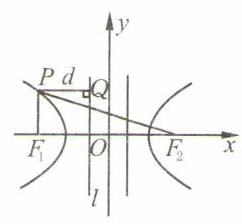
\includegraphics[width=0.2\textwidth]{bodyxb/src/bo_d20aucref24c73anc48g_88_1270_441_242_224_0.jpg}
\end{center}


(第 139 题)

140. (1) 已知 $P,Q$ 分别是椭圆 $9{x}^{2} + 4{y}^{2} = {36}$ 的两个焦点,点 $M$ 在双曲线 $9{x}^{2} - {25}{y}^{2} = {225}$ 上,求 $\bigtriangleup {PQM}$ 重心的轨迹方程;

(2)已知过点 $A\left( {2,1}\right)$ 的直线与曲线 $2{x}^{2} - {y}^{2} = 2$ 交于 $P,Q$ 两点,求线段 ${PQ}$ 中点 $M$ 的轨迹方程;

(3)已知点 $B\left( {-6,0}\right) ,C\left( {6,0}\right)$ 是 $\bigtriangleup  {ABC}$ 的两个顶点,内角 $A,B,C$ 满足 $\sin B - \sin C =$  $\dfrac{1}{2}\sin A$ ,求顶点 $A$ 的轨迹方程；

(4)已知以动点 $P$ 为圆心的圆与两圆 ${\left( x + 5\right) }^{2} + {y}^{2} = {49}$ 和 ${\left( x - 5\right) }^{2} + {y}^{2} = 1$ 都外切,求动点 $P$ 的轨迹方程;

(5)过原点的双曲线有一个焦点为 $F\left( {4,0}\right)$ ,实轴长为 4,求双曲线中心的轨迹方程；

(6)已知点 $P,Q$ 分别在射线 $y = x\left( {x > 0}\right)$ 和 $y =  - x\left( {x > 0}\right)$ 上,且 $\bigtriangleup {POQ}$ 的面积为 1 ( $O$ 为原点),求线段 ${PQ}$ 的中点 $M$ 的轨迹方程.

141. (1) 过点 $A\left( {1,1}\right)$ 作双曲线 ${x}^{2} - 4{y}^{2} = {16}$ 的弦,此弦被点 $A$ 平分,求这条弦所在直线的方程;

(2)过点 $P\left( {-2,2}\right)$ 的直线被双曲线 ${x}^{2} - 2{y}^{2} = 8$ 截得的弦 ${MN}$ 的中点恰好为 $P$ ,求 $\left| {MN}\right|$ 的值;

(3)已知双曲线 $2{x}^{2} - {y}^{2} = 2$ ,试问过点 $N\left( {1,1}\right)$ 能否作一直线与双曲线交于 $C,D$ 两点, 且使 $N$ 为 ${CD}$ 的中点? 这样的直线如果存在,求出它的方程; 如果不存在,请说明其理由.

142. 已知直线 $y = x + b$ 与双曲线 $2{x}^{2} - {y}^{2} = 2$ 相交于 $A,B$ 两点,若以 ${AB}$ 为直径的圆过原点,求 $b$ 的值.

143. 已知中心都在原点,焦点都在 $x$ 轴上的椭圆与双曲线有共同的焦点 ${F}_{1},{F}_{2}$ ,且 $\left| {{F}_{1}{F}_{2}}\right|  =$  $2\sqrt{13}$ ,又椭圆的长半轴长与双曲线的实半轴长之差等于 4 ,且它们的离心率之比为 $3 : 7$ .

(1)求椭圆和双曲线的方程；

(2)若 $P$ 是它们的一个公共点,求 $\angle {F}_{1}P{F}_{2}$ 的余弦值.

\section*{(B)}

144. 已知椭圆 $\dfrac{{x}^{2}}{{a}^{2}} + \dfrac{{y}^{2}}{{b}^{2}} = 1\left( {a > b > 0}\right)$ 和双曲线 $\dfrac{{x}^{2}}{{m}^{2}} - \dfrac{{y}^{2}}{{n}^{2}} = 1\left( {m,n > 0}\right)$ 有公共的焦点 ${F}_{1},{F}_{2},P$ 是两曲线的一个公共点.

(1) 求 $\left| {P{F}_{1}}\right|  \cdot  \left| {P{F}_{2}}\right|$ ; (2)求证: $\angle {F}_{1}P{F}_{2} = 2\arctan \dfrac{n}{b}$ ；

(3) 求证: $\bigtriangleup {F}_{1}P{F}_{2}$ 的面积 $= {bn}$ .

* 145. 已知 ${AB}$ 是双曲线 $\dfrac{{x}^{2}}{{a}^{2}} - \dfrac{{y}^{2}}{{b}^{2}} = 1$ 过焦点 ${F}_{1}$ 的任意一条弦,以 ${AB}$ 为直径的圆被 ${F}_{1}$ 相应的准线截得的圆弧为 $\overset{⏜}{MN}$ ,求证: $\overset{⏜}{MN}$ 的度数为定值.

\section*{五、抛物线}

\section*{(一) 抛物线的基本性质}

\section*{【典型题型和解题技巧】}

1. 抛物线的焦点位置.

和椭圆、双曲线一样, 抛物线焦点位置的确定十分重要, 它是正确求解与抛物线基本性质有关的问题的前提.

\begin{center}
\adjustbox{width=\textwidth}{
\begin{tabular}{|c|c|c|c|c|}
\hline
焦点的位置 & 图 形 & 方 程 & 焦 点 & 准 线 \\
\cline{1-5}
焦点在 $x$ 正半轴 &  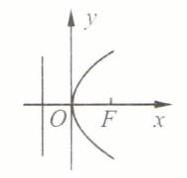
\includegraphics[width=0.2\textwidth]{bodyxb/src/bo_d20aucref24c73anc48g_89_393_1382_187_178_0.jpg}  & ${y}^{2} = {2px}\left( {p > 0}\right)$ & $\left( {\dfrac{p}{2},0}\right)$ & $x =  - \dfrac{p}{2}$ \\
\cline{1-5}
焦点在 $x$ 负半轴 &  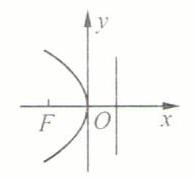
\includegraphics[width=0.2\textwidth]{bodyxb/src/bo_d20aucref24c73anc48g_89_391_1585_195_179_0.jpg}  & ${y}^{2} =  - {2px}\left( {p > 0}\right)$ & $\left( {-\dfrac{p}{2},0}\right)$ & $x = \dfrac{p}{2}$ \\
\cline{1-5}
焦点在 $y$ 正半轴 &  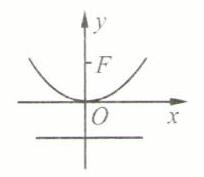
\includegraphics[width=0.2\textwidth]{bodyxb/src/bo_d20aucref24c73anc48g_89_389_1789_204_177_0.jpg}  & ${x}^{2} = {2py}\left( {p > 0}\right)$ & $\left( {0,\dfrac{p}{2}}\right)$ & $y =  - \dfrac{p}{2}$ \\
\cline{1-5}
焦点在 $y$ 负半轴 &  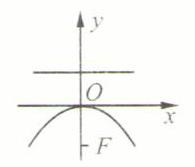
\includegraphics[width=0.2\textwidth]{bodyxb/src/bo_d20aucref24c73anc48g_89_394_1990_195_167_0.jpg}  & ${x}^{2} =  - {2py}\left( {p > 0}\right)$ & $\left( {0, - \dfrac{p}{2}}\right)$ & $y = \dfrac{p}{2}$ \\
\cline{1-5}
\hline
\end{tabular}
}
\end{center}

例 1 求 $y = \dfrac{1}{3}{x}^{2}$ 的焦点坐标和准线方程.

解 由已知得 ${x}^{2} = {3y}$ ,即 ${x}^{2} = 2 \cdot  \dfrac{3}{2}y,\therefore \dfrac{p}{2} = \dfrac{3}{4}$ ,且抛物线的焦点在 $y$ 正半轴,

$\therefore$ 焦点为 $P\left( {0,\dfrac{3}{4}}\right)$ ; 准线方程为 $y =  - \dfrac{3}{4}$ .

2. 利用抛物线的定义解题.

根据抛物线的定义可知: 抛物线上的点到抛物线的焦点和准线等距离.

一些与抛物线的焦半径、焦点弦以及准线有关的问题, 常常可以利用抛物线这一定义求解.

例 2 已知 $P\left( {{x}_{0},{y}_{0}}\right)$ 是抛物线 ${y}^{2} = {2px}\left( {p > 0}\right)$ 上的点, $F$ 是此抛物线的焦点,求证: $\left| {PF}\right|  = {x}_{0} + \dfrac{p}{2}$ .

\begin{center}
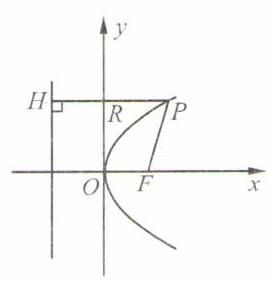
\includegraphics[width=0.2\textwidth]{bodyxb/src/bo_d20aucref24c73anc48g_90_1221_677_270_281_0.jpg}
\end{center}


(图 27)

证明 如图 27, $x =  - \dfrac{p}{2}$ 是抛物线的准线,过点 $P$ 作准线的垂线,垂足为 $H,{PH}$ 交 $y$ 轴于点 $R$ ,则 $\left| {PF}\right|  = \left| {PH}\right|  = \left| {PR}\right|  + \left| {RH}\right|  = {x}_{0} + \dfrac{p}{2}$ .

例 3 已知 $F$ 是抛物线 ${y}^{2} = {4x}$ 的焦点, $A\left( {3,2}\right)$ 是一个定点, $P$ 是抛物线上的动点 (如图 28),求 $\left| {PA}\right|  + \left| {PF}\right|$ 的最小值及此时点 $P$ 的坐标.

解 设抛物线的准线为 $l$ ,过点 $P$ 作 ${PH} \bot  l$ ,垂足为 $H$ ,再过点 $A$ 作 $A{H}^{\prime } \bot  l$ ,垂足为 ${H}^{\prime }$ ,并交抛物线于点 ${P}^{\prime }$ . 连接 ${P}^{\prime }F,{PF}$ ,则

\[
\left| {PA}\right|  + \left| {PF}\right|  = \left| {PA}\right|  + \left| {PH}\right|  \geq  \left| {A{H}^{\prime }}\right|  = \left| {{P}^{\prime }A}\right|  + \left| {{P}^{\prime }{H}^{\prime }}\right|
\]

\begin{center}
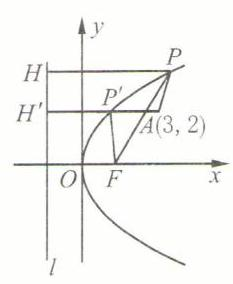
\includegraphics[width=0.2\textwidth]{bodyxb/src/bo_d20aucref24c73anc48g_90_1258_1139_233_284_0.jpg}
\end{center}


(图 28)

$= \left| {{P}^{\prime }A}\right|  + \left| {{P}^{\prime }F}\right|$ ,

$\therefore \left| {PA}\right|  + \left| {PF}\right|$ 的最小值是 $\left| {A{H}^{\prime }}\right|$ ,而准线 $l$ 的方程为 $x =  - 1$ ,

故 $\left| {PA}\right|  + \left| {PF}\right|$ 的最小值是 4,此时,点 ${P}^{\prime }$ 的纵坐标为 2,代入抛物线方程得点 ${P}^{\prime }$ 的横坐标是 1 . 故此时点 $P$ 的坐标为 (1,2).

\section*{【训练题】}

\section*{(A)}

146. 若 $A$ 是定直线 $l$ 外的一定点,则过点 $A$ 且与 $l$ 相切的圆的圆心轨迹是 (   )

(A) 圆. (B) 椭圆. (C) 双曲线一支. (D) 抛物线.

147. 抛物线 ${y}^{2} = {10x}$ 的焦点到准线的距离是(   )

(A) 2.5 . (B) 5. (C) 7.5. (D) 10.

148. 已知原点为顶点, $x$ 轴为对称轴的抛物线的焦点在直线 ${2x} - {4y} + {11} = 0$ 上,则此抛物线的方程是(   )

(A) ${y}^{2} = {11x}$ . (B) ${y}^{2} =  - {11x}$ . (C) ${y}^{2} = {22x}$ . (D) ${y}^{2} =  - {22x}$ .

149. 抛物线 $x = a{y}^{2}\left( {a \neq  0}\right)$ 的焦点坐标为(   )

(A) $\left( {\dfrac{1}{a},0}\right)$ . (B) $\left( {\dfrac{1}{2a},0}\right)$ .

(C) $\left( {\dfrac{1}{4a},0}\right)$ . (D) $a > 0$ 时为 $\left( {\dfrac{1}{4a},0}\right) ,a < 0$ 时为 $\left( {-\dfrac{1}{4a},0}\right)$ .

150. 抛物线 $y = 4{x}^{2}$ 的准线方程是(   )

(A) $x =  - 1$ . (B) $y =  - 1$ .

(C) $x =  - \dfrac{1}{16}$ . (D) $y =  - \dfrac{1}{16}$ .

151. 若点 $P$ 到点 $F\left( {4,0}\right)$ 的距离比它到定直线 $x + 5 = 0$ 的距离小 1 ,则点 $P$ 的轨迹方程是(   )

(A) ${y}^{2} =  - {16x}$ . (B) ${y}^{2} =  - {32x}$ . (C) ${y}^{2} = {16x}$ . (D) ${y}^{2} = {32x}$ .

152. (1)顶点在原点,过点(-2,3)的抛物线的标准方程为\blkda{}；

(2)顶点在原点,焦点在 $x$ 轴上且通径(过焦点和对称轴垂直的弦)长为 6 的抛物线方程是\blkda{}；

(3)抛物线顶点在原点,焦点在 $x$ 轴上,其通径的两端点与顶点连成的三角形面积为 4, 则此抛物线方程为\blkda{}；

(4)已知椭圆以抛物线 ${y}^{2} = {4x}$ 的顶点为中心,以此抛物线的焦点为右焦点,又椭圆的短轴长为 2,则此椭圆方程为\blkda{}.

153. (1) 在抛物线 ${y}^{2} = {8x}$ 上有一点 $P$ ,它到焦点的距离是 20,则点 $P$ 的坐标是\blkda{};

(2)已知抛物线 ${y}^{2} = {4ax}\left( {a > 0}\right)$ 上一点 $A\left( {m,n}\right)$ 到焦点 $F$ 的距离等于 ${4a}$ ,则 $m =$ \blkda{}, $n =$ \blkda{};

(3)抛物线 ${y}^{2} = {16x}$ 上一点 $P$ 到 $x$ 轴的距离为 12 ,则点 $P$ 与焦点 $F$ 的距离 $\left| {PF}\right|$  $=$ \blkda{};

(4)已知抛物线顶点在原点,焦点在 $y$ 轴上,又抛物线上一点(m, - 3)到焦点的距离为 5,则 $m =$ \blkda{},此抛物线方程为\blkda{}.

154. (1) 抛物线 ${y}^{2} = {2x}$ 的焦点弦的端点为 $A\left( {{x}_{1},{y}_{1}}\right) ,B\left( {{x}_{2},{y}_{2}}\right)$ ,且 ${x}_{1} + {x}_{2} = 3$ ,则 $\left| {AB}\right|$  $=$ \blkda{};

(2)若以曲线 $\dfrac{{x}^{2}}{25} + \dfrac{{y}^{2}}{16} = 1$ 的中心为顶点,直线 $x =  - \dfrac{25}{3}$ 为准线的抛物线与直线 $x = \dfrac{25}{3}$ 交于 $A,B$ 两点,则 $\left| {AB}\right|  =$ \blkda{}；

(3)若正三角形的一个顶点在原点,另两个顶点在抛物线 ${y}^{2} = {2px}\left( {p > 0}\right)$ 上,则这个三角形的面积为\blkda{}；

(4)过抛物线 ${y}^{2} = {2px}$ 的对称轴上一点 $C\left( {p,0}\right)$ 作一条直线与抛物线交于 $A,B$ 两点,若点 $A$ 的纵坐标为 $- \dfrac{p}{2}$ ,则点 $B$ 的纵坐标为\blkda{}.

\section*{(B)}

155. (1) 若顶点在原点,焦点在 $x$ 轴上的抛物线截直线 $y = {2x} + 1$ 所得的弦长为 $\sqrt{15}$ ,求此抛物线的方程;

(2)若直线 $y = {kx} - 2$ 交抛物线 ${y}^{2} = {8x}$ 于 $A,B$ 两点,且 ${AB}$ 中点的横坐标是 2, 求 $\left| {AB}\right|$ .

156. (1) 已知抛物线 ${y}^{2} = {4x}$ 截直线 $y = {2x} + b$ 所得的弦长 $\left| {AB}\right|  = 3\sqrt{5}$ ,试在 $x$ 轴上求一点 $P$ ,使 $\bigtriangleup {ABP}$ 的面积为 39;

(2)求证:抛物线 ${y}^{2} = {2px}\left( {p > 0}\right)$ 的焦点弦长 $\left| {AB}\right|  = \dfrac{2p}{{\sin }^{2}\theta }$ (其中 $\theta$ 为直线 ${AB}$ 的倾斜角);

(3)若 ${y}^{2} = {4x}$ 的焦点弦长为 5 ,求焦点弦所在直线方程.

\section*{(二) 抛物线的综合应用}

\section*{【典型题型和解题技巧】}

1. 韦达定理的应用.

例 1 已知抛物线 ${y}^{2} = {2px}\left( {p > 0}\right)$ 与圆 ${\left( x - 2\right) }^{2} + {y}^{2} = 3$ 相交, $A,B$ 是它们在 $x$ 轴上方的公共点 (如图 29),若线段 ${AB}$ 的中点 $M$ 在直线 $y = x$ 上,求 $p$ 的值.

解 考虑方程组 $\left\{  \begin{array}{l} {y}^{2} = {2px}, \\  {\left( x - 2\right) }^{2} + {y}^{2} = 3, \end{array}\right.$

\begin{center}
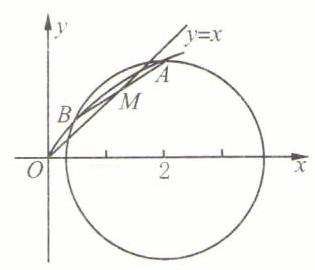
\includegraphics[width=0.2\textwidth]{bodyxb/src/bo_d20aucref24c73anc48g_92_1191_1222_315_270_0.jpg}
\end{center}


(图 29)

消去 $y$ 并整理得 ${x}^{2} + \left( {{2p} - 4}\right) x + 1 = 0$ .

设 $A\left( {{x}_{1},{y}_{1}}\right) ,B\left( {{x}_{2},{y}_{2}}\right)$ ,则有 $\left\{  \begin{array}{l} {x}_{1} + {x}_{2} = 4 - {2p} > 0, \\  {x}_{1}{x}_{2} = 1. \end{array}\right.$

设 ${AB}$ 的中点为 $M\left( {{x}_{0},{y}_{0}}\right)$ ,则

${x}_{0} = \dfrac{{x}_{1} + {x}_{2}}{2} = 2 - p,$

${y}_{0} = \dfrac{{y}_{1} + {y}_{2}}{2} = \dfrac{\sqrt{2p}}{2}\left( {\sqrt{{x}_{1}} + \sqrt{{x}_{2}}}\right)  = \dfrac{\sqrt{2p}}{2}\sqrt{{\left( \sqrt{{x}_{1}} + \sqrt{{x}_{2}}\right) }^{2}} = \dfrac{\sqrt{2p}}{2}\sqrt{{x}_{1} + {x}_{2} + 2\sqrt{{x}_{1}{x}_{2}}} =$  $\dfrac{\sqrt{2p}}{2}\sqrt{6 - {2p}} = \sqrt{p\left( {3 - p}\right) }.$

$\because$ 点 $M\left( {{x}_{0},{y}_{0}}\right)$ 在直线 $y = x$ 上,

$\therefore 2 - p = \sqrt{p\left( {3 - p}\right) }$ ,整理得 $2{p}^{2} - {7p} + 4 = 0$ ,解得 $p = \dfrac{7 \pm  \sqrt{17}}{4}$ .

又 $\because 4 - {2p} > 0,\therefore 0 < p < 2,\therefore p = \dfrac{7 - \sqrt{17}}{4}$ .

例 2 若抛物线 $y = {x}^{2}$ 上存在两点关于直线 $y = m\left( {x - 3}\right)$ 对称,求 $m$ 的取值范围.

解 如图 30,设抛物线上两点 $A\left( {{x}_{1},{y}_{1}}\right) ,B\left( {{x}_{2},{y}_{2}}\right)$ 关于直线 $y = m$ (x - 3)对称, ${AB}$ 的中点为 $M\left( {{x}_{0},{y}_{0}}\right)$ .

\begin{center}
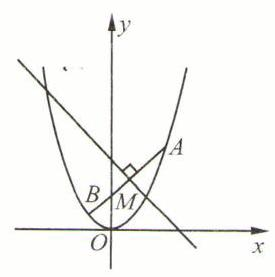
\includegraphics[width=0.2\textwidth]{bodyxb/src/bo_d20aucref24c73anc48g_93_1151_142_275_277_0.jpg}
\end{center}


(图 30)

显然 $m \neq  0$ ,则

${k}_{AB} = \dfrac{{y}_{2} - {y}_{1}}{{x}_{2} - {x}_{1}} = \dfrac{{x}_{2}^{2} - {x}_{1}^{2}}{{x}_{2} - {x}_{1}} = {x}_{2} + {x}_{1} =  - \dfrac{1}{m},$①

$\therefore {x}_{0} = \dfrac{{x}_{1} + {x}_{2}}{2} =  - \dfrac{1}{2m},$

${y}_{0} = \dfrac{{y}_{1} + {y}_{2}}{2} = \dfrac{{\left( {x}_{1} + {x}_{2}\right) }^{2} - 2{x}_{1}{x}_{2}}{2} = \dfrac{\dfrac{1}{{m}^{2}} - 2{x}_{1}{x}_{2}}{2}.$

将 $\left( {{x}_{0},{y}_{0}}\right)$ 代入方程 $y = m\left( {x - 3}\right)$ ,得 ${x}_{1}{x}_{2} = \dfrac{1}{2{m}^{2}} + \dfrac{1}{2} + {3m}$ .

由①,②知, ${x}_{1},{x}_{2}$ 是方程 ${t}^{2} + \dfrac{1}{m}t + \left( {\dfrac{1}{2{m}^{2}} + \dfrac{1}{2} + {3m}}\right)  = 0$ 的根.

由 $\Delta  > 0$ ,得 $\left( {{2m} + 1}\right) \left( {6{m}^{2} - {2m} + 1}\right)  < 0,\therefore m <  - \dfrac{1}{2}$ .

注意 韦达定理在解析几何中应用极为广泛, 当直线与二次曲线相交时, 常可利用韦达定理觅得解题途径.

本例还可以用如下方法解得:

先求出斜率为 $- \dfrac{1}{m}$ 的平行弦的中点轨迹 $C$ ,即直线 $x =  - \dfrac{1}{2m}$ ; 再求轨迹 $C$ 与直线 $y = m(x -$

3)的公共点 $\left( {{x}_{0},{y}_{0}}\right)$ , $\left\{  \begin{array}{l} {x}_{0} =  - \dfrac{1}{2m}, \\  {y}_{0} = m\left( {-\dfrac{1}{2m} - 3}\right) . \end{array}\right.$ 由题设,点 $\left( {{x}_{0},{y}_{0}}\right)$ 应在抛物线 $y = {x}^{2}$ 内部,故 ${y}_{0} > {x}_{0}^{2}$ ,

$\therefore m\left( {-\dfrac{1}{2m} - 3}\right)  > \dfrac{1}{4{m}^{2}}$ (下略).

2. 抛物线的标点法.

对于抛物线 ${y}^{2} = {2px}$ 上的点,通常有三种标点方法:

(1) 设 $P\left( {{x}_{0},{y}_{0}}\right)$ 且 ${y}_{0}^{2} = {2p}{x}_{0}$ ;

(2) 设 $P\left( {\dfrac{{y}_{0}^{2}}{2p},{y}_{0}}\right)$ ;

(3) 设 $P\left( {{2p}{t}^{2},{2pt}}\right)$ .

例 3 设 $A,B$ 是抛物线 ${y}^{2} = {2px}$ 上的点,且满足 $\angle {AOB} = {90}^{ \circ  }(O$ 是坐标原点)(如图 31).

\begin{center}
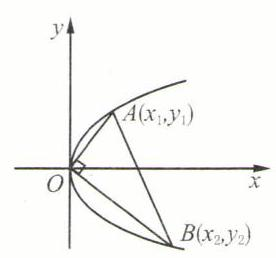
\includegraphics[width=0.2\textwidth]{bodyxb/src/bo_d20aucref24c73anc48g_93_1139_1844_276_258_0.jpg}
\end{center}


(图 31)

求证: 直线 ${AB}$ 过定点,并求此定点.

证法一 设 $A\left( {{x}_{1},{y}_{1}}\right) ,B\left( {{x}_{2},{y}_{2}}\right)$ ,则 ${y}_{1}^{2} = {2p}{x}_{1},{y}_{2}^{2} = {2p}{x}_{2}$ .

$\because \angle {AOB} = {90}^{ \circ  },\therefore \dfrac{{y}_{1}{y}_{2}}{{x}_{1}{x}_{2}} =  - 1$ ,即 ${y}_{1}{y}_{2} =  - {x}_{1}{x}_{2} =  - \dfrac{{y}_{1}^{2}{y}_{2}^{2}}{4{p}^{2}}$ ,

$\therefore {y}_{1}{y}_{2} =  - 4{p}^{2}$ .

再由直线 $l : y - {y}_{1} = \dfrac{{y}_{2} - {y}_{1}}{{x}_{2} - {x}_{1}}\left( {x - {x}_{1}}\right)$ ,

得 $y - {y}_{1} = \dfrac{2p}{{y}_{2} + {y}_{1}}\left( {x - {x}_{1}}\right)$ ,即 $\left( {{y}_{2} + {y}_{1}}\right) y - {y}_{1}{y}_{2} - {y}_{1}^{2} = {2px} - {2p}{x}_{1}$ .

$\because {y}_{1}^{2} = {2p}{x}_{1},{y}_{1}{y}_{2} =  - 4{p}^{2},\therefore \left( {{y}_{2} + {y}_{1}}\right) y + 4{p}^{2} = {2px}$ ,

即 $\left( {{y}_{2} + {y}_{1}}\right) y = {2p}\left( {x - {2p}}\right)$ . 故直线 ${AB}$ 恒过定点(2p,0).

证法二 设 $A\left( {{2p}{a}^{2},{2pa}}\right) ,B\left( {{2p}{b}^{2},{2pb}}\right)$ ,则由 $\angle {AOB} = {90}^{ \circ  }$ ,得 $\dfrac{{2pa} \cdot  {2pb}}{{2p}{a}^{2} \cdot  {2p}{b}^{2}} =  - 1$ ,

即 ${ab} =  - 1$ .

再由直线 $l : y - {2pa} = \dfrac{{2pb} - {2pa}}{{2p}{b}^{2} - {2p}{a}^{2}}\left( {x - {2p}{a}^{2}}\right)$ ,得 $y - {2pa} = \dfrac{1}{b + a}\left( {x - {2p}{a}^{2}}\right)$ ,

即 $\left( {a + b}\right) y - {2pab} - {2p}{a}^{2} = x - {2p}{a}^{2}$ .

$\because {ab} =  - 1,\therefore \left( {a + b}\right) y + {2p} = x$ ,即 $\left( {a + b}\right) y = x - {2p}$ ,

$\therefore$ 直线 ${AB}$ 恒过定点(2p,0).

\section*{【训练题】}

\section*{(A)}

157. 若抛物线 ${y}^{2} = {2px}\left( {p > 0}\right)$ 的弦 ${PQ}$ 的中点为 $\left( {{x}_{0},{y}_{0}}\right) \left( {{y}_{0} \neq  0}\right)$ ,则弦 ${PQ}$ 的斜率为(   )

(A) $- \dfrac{p}{{x}_{0}}$ . (B) $\dfrac{p}{{y}_{0}}$ . (C) $p{x}_{0}$ . (D) $- p{x}_{0}$ .

158. 若 ${AB}$ 是抛物线 ${y}^{2} = {4x}$ 的焦点弦,其坐标 $A\left( {{x}_{1},{y}_{1}}\right) ,B\left( {{x}_{2},{y}_{2}}\right)$ 满足 ${x}_{1} + {x}_{2} = 6$ ,则直线 ${AB}$ 的斜率是(   )

(A) $\pm  \dfrac{1}{2}$ . (B) $\pm  \dfrac{\sqrt{2}}{2}$ .

(C) $\pm  1$ . (D) $\pm  \sqrt{2}$ .

159. 若抛物线 ${y}^{2} = {2px}\left( {p > 0}\right)$ 的焦点弦 ${AB}$ 的两端点坐标分别为 $A\left( {{x}_{1},{y}_{1}}\right) ,B\left( {{x}_{2},{y}_{2}}\right)$ ,则 $\dfrac{{y}_{1}{y}_{2}}{{x}_{1}{x}_{2}}$ 的值一定等于(   )

(A) 4. (B) -4. (C) ${p}^{2}$ . (D) $- {p}^{2}$ .

160. 若 $\odot  M$ 的圆心在抛物线 $C : y = \dfrac{1}{4}{x}^{2}$ 上,且 $\odot  M$ 与 $y$ 轴及 $C$ 的准线相切,则 $\odot  M$ 的方程是(   )

(A) ${x}^{2} + {y}^{2} \pm  {4x} - {2y} - 1 = 0$ . (B) ${x}^{2} + {y}^{2} \pm  {4x} - {2y} + 1 = 0$ .

(C) ${x}^{2} + {y}^{2} \pm  {4x} - {2y} - 4 = 0$ . (D) ${x}^{2} + {y}^{2} \pm  {4x} - {2y} + 4 = 0$ .

161. 设抛物线 $y = a{x}^{2}\left( {a > 0}\right)$ 与直线 $y = {kx} + b$ 相交于两点,它们的横坐标为 ${x}_{1},{x}_{2}$ ,而 ${x}_{3}$ 是直线与 $x$ 轴交点的横坐标,那么 ${x}_{1},{x}_{2},{x}_{3}$ 的关系是 (   )

(A) ${x}_{3} = {x}_{1} + {x}_{2}$ . (B) ${x}_{3} = \dfrac{1}{{x}_{1}} + \dfrac{1}{{x}_{2}}$ .

(C) ${x}_{1}{x}_{2} = {x}_{2}{x}_{3} + {x}_{3}{x}_{1}$ . (D) ${x}_{1}{x}_{3} = {x}_{2}{x}_{3} + {x}_{1}{x}_{2}$ .

162. 当 $0 < k < \dfrac{1}{3}$ 时,关于 $x$ 的方程 $\sqrt{\left| 2 - x\right| } = {kx}$ 的实数解的个数是(   )

(A) 0 . (B) 1 . (C) 2 . (D) 3 .

163. 将直线 $x - {2y} + b = 0$ 向左平移 1 个单位,再向下平移 2 个单位后,它与抛物线 ${y}^{2} = {4x}$ 仅有一个公共点,则实数 $b$ 的值等于 (   )

(A) -1 . (B) 1 . (C) 7. (D) 9.

\section*{(B)}

164. 抛物线 ${y}^{2} =  - {4x}$ 关于直线 $x + y - 2 = 0$ 对称的曲线的顶点坐标是 (   )

(A)(0,0). (B)(-2, - 2).

(C)(2,2). (D)(2,0).

165. 抛物线 ${y}^{2} = x$ 上的点到直线 $x - {2y} + 4 = 0$ 的距离最小的是点 (   )

(A) $\left( {\dfrac{1}{4},\dfrac{1}{2}}\right)$ . (B) $\left( {\dfrac{9}{4},\dfrac{3}{2}}\right)$ . (C)(1,1). (D)(4,2).

166. 已知抛物线 ${y}^{2} = {2px}\left( {p > 0}\right)$ 上有一点 $M\left( {4,y}\right)$ ,它到焦点 $F$ 的距离为 5,则 $\bigtriangleup {OFM}$ 的面积 $\left( {O\text{ 为原点 }}\right)$ 为(   )

(A) 1 . (B) $\sqrt{2}$ . (C) 2 . (D) $2\sqrt{2}$ .

167. 记定点 $M\left( {3,\dfrac{10}{3}}\right)$ 与抛物线 ${y}^{2} = {2x}$ 上的点 $P$ 之间的距离为 ${d}_{1}$ ,点 $P$ 到此抛物线准线 $l$ 的距离为 ${d}_{2}$ ,则当 ${d}_{1} + {d}_{2}$ 取最小值时点 $P$ 的坐标为(   )

(A)(0,0). (B) $\left( {1,\sqrt{2}}\right)$ . (C)(2,2). (D) $\left( {\dfrac{1}{2},1}\right)$ .

168. 若点 $P$ 在抛物线 ${y}^{2} = x$ 上,点 $Q$ 在圆 ${\left( x - 3\right) }^{2} + {y}^{2} = 1$ 上,则 $\left| {PQ}\right|$ 的最小值等于 (   )

(A) $\sqrt{3} - 1$ . (B) $\dfrac{\sqrt{10}}{2} - 1$ . (C) 2 . (D) $\dfrac{1}{2}\left( {\sqrt{11} - 2}\right)$ .

169. (1) 过点(0, - 4)且与直线 $y = 4$ 相切的圆的圆心的轨迹方程是\blkda{}；

(2)与 $y$ 轴相切,且与圆 ${x}^{2} + {y}^{2} - {4x} = 0$ 外切的圆的圆心的轨迹方程是\blkda{}.

170. (1) 抛物线 ${y}^{2} =  - {8x}$ 被点 $P\left( {-1,1}\right)$ 所平分的弦的直线方程为\blkda{}；

(2)已知抛物线 ${y}^{2} = {2x}$ 的弦 ${AB}$ 过定点(-2,0),则弦 ${AB}$ 中点的轨迹方程是\blkda{}；

(3)抛物线 $y = 2{x}^{2}$ 的一组斜率为 2 的平行弦的中点轨迹方程是\blkda{}.

171. (1) 已知过抛物线焦点 $F$ 的直线与抛物线相交于 $A,B$ 两点, 点 $A,B$ 在此抛物线准线上的射影分别为 ${A}_{1},{B}_{1}$ (如图),求证: $\angle {A}_{1}F{B}_{1} = {90}^{ \circ  }$ ;

\begin{center}
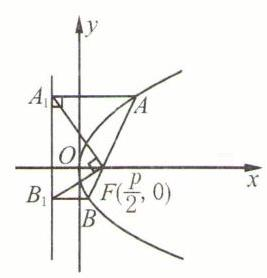
\includegraphics[width=0.2\textwidth]{bodyxb/src/bo_d20aucref24c73anc48g_96_1255_151_267_278_0.jpg}
\end{center}


[第 171(1)题]

(2)已知直线 $\sqrt{3}x + {2y} - 6 = 0$ 与抛物线 ${y}^{2} = 2\sqrt{3}x$ 相交于 $P$ , $Q$ 两点,求证: $\angle {POQ} = {90}^{ \circ  }$ ( $O$ 为坐标原点);

(3)已知抛物线 ${y}^{2} = {2px}\left( {p > 0}\right)$ ,求证:在 $x$ 轴上存在一点 $M$ ,使得过点 $M$ 的弦 ${P}_{1}{P}_{2}$ 总满足 $\angle {P}_{1}O{P}_{2} = {90}^{ \circ  }$ .

172. (1) 已知 $A$ 为抛物线 ${y}^{2} = {2px}$ 上的一点, ${BC}$ 是垂直于 $x$ 轴的一条弦,直线 ${AC}$ 交抛物线的对称轴于点 $E$ ,直线 ${AB}$ 交抛物线的对称轴于点 $D$ (如图),求证: 抛物线的顶点平分线段 ${DE}$ ；

\begin{center}
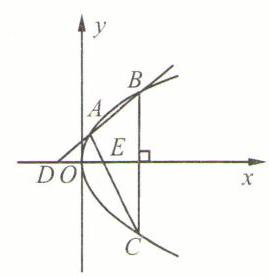
\includegraphics[width=0.2\textwidth]{bodyxb/src/bo_d20aucref24c73anc48g_96_1251_560_269_278_0.jpg}
\end{center}


[第 172(1)题]

(2)已知 $A\left( {{x}_{1},{y}_{1}}\right) ,B\left( {{x}_{2},{y}_{2}}\right)$ 是抛物线 ${y}^{2} = {2px}\left( {p > 0}\right)$ 上两点,过线段 ${AB}$ 的中点 $M$ 作抛物线对称轴的平行线与抛物线交于点 $C\left( {{x}_{3},{y}_{3}}\right)$ ,求证: $\bigtriangleup {ABC}$ 的面积等于 $\dfrac{1}{16p}{\left| {y}_{1} - {y}_{2}\right| }^{3}$ ;

(3)已知 ${PQ}$ 是垂直于 $x$ 轴的抛物线 ${y}^{2} = {2px}\left( {p > 0}\right)$ 的焦点弦, $M$ 是 ${FP}$ 的中点 $(F$ 为焦点),过点 $M$ 作直线与抛物线交于点 $A,B$ ,若 $\bigtriangleup {PMA}$ 的面积与 $\bigtriangleup {QMB}$ 的面积相等,求直线 ${AB}$ 的方程和弦 ${AB}$ 的长;

(4)过抛物线焦点 $F$ 的直线交此抛物线于 $P$ , $Q$ 两点,弦 ${PQ}$ 的垂直平分线交此曲线的对称轴于点 $R$ (如图),求证: $\left| {FR}\right|  = \dfrac{1}{2}\left| {PQ}\right|$ ;

(5)已知 $\bigtriangleup  {AOB}$ 是以原点 $O$ 为直角顶点的抛物线 ${x}^{2} = {2py}\left( {p > 0}\right)$ 的内接直角三角形 (如图),求 $\bigtriangleup  {AOB}$ 面积的最小值;

(6)已知 $F$ 是抛物线 ${y}^{2} = {8x}$ 的焦点,一条倾斜角为 $\dfrac{\pi }{4}$ 的弦 ${AB}$ 长为 $8\sqrt{5}$ (如图),求 $\bigtriangleup {FAB}$ 的面积和 $\sin \angle {AFB}$ 的值.

\begin{center}
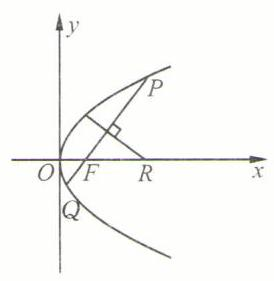
\includegraphics[width=0.2\textwidth]{bodyxb/src/bo_d20aucref24c73anc48g_96_341_1650_274_281_0.jpg}
\end{center}


[第 172(4)题]

\begin{center}
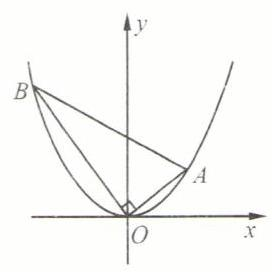
\includegraphics[width=0.2\textwidth]{bodyxb/src/bo_d20aucref24c73anc48g_96_743_1657_272_272_0.jpg}
\end{center}


[第 172(5)题]

\begin{center}
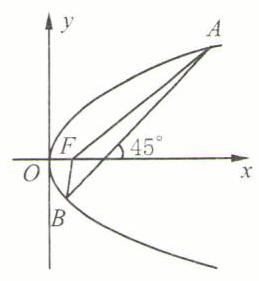
\includegraphics[width=0.2\textwidth]{bodyxb/src/bo_d20aucref24c73anc48g_96_1145_1650_259_281_0.jpg}
\end{center}


[第 172(6)题]

173. (1) 已知正方形的一条边 ${AB}$ 在直线 $y = x + 4$ 上,顶点 $C,D$ 在抛物线 ${y}^{2} = x$ 上 (如图), 求正方形的边长;

(2)过点 $P\left( {{11},0}\right)$ 作倾角为 $\dfrac{\pi }{4}$ 的直线交抛物线 ${y}^{2} = {4x}$ 于 $R,Q$ 两点,再作与 ${RQ}$ 平行的直线交抛物线的 $\overset{⏜}{ROQ}$ 于点 $M,N$ (如图),求 $\bigtriangleup {PMN}$ 面积的最大值.

\begin{center}
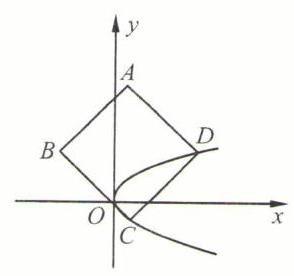
\includegraphics[width=0.2\textwidth]{bodyxb/src/bo_d20aucref24c73anc48g_97_325_311_294_276_0.jpg}
\end{center}


[第 173(1)题]

\begin{center}
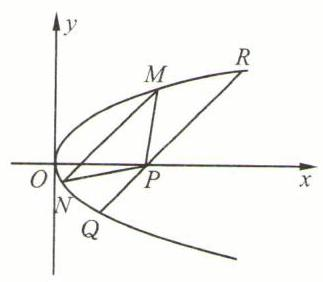
\includegraphics[width=0.2\textwidth]{bodyxb/src/bo_d20aucref24c73anc48g_97_850_309_323_282_0.jpg}
\end{center}


[第 173(2)题]

174. (1) 设抛物线 ${y}^{2} = x$ 的弦 ${PQ}$ 被直线 $l : x + y - 2 = 0$ 垂直平分,求 $\bigtriangleup {OPQ}$ 的面积 $(O$ 为原点)；

(2) $k$ 为何值时,直线 $y - 1 = k\left( {x - 1}\right)$ 能垂直平分抛物线 ${y}^{2} = x$ 的一条弦 ${AB}$ ？

175. 抛物线 ${y}^{2} = {2x}$ 上的点 $P\left( {x,y}\right)$ 到点 $A\left( {a,0}\right) \left( {a \in  \mathbf{R}}\right)$ 的距离的最小值记为 $f\left( a\right)$ .

(1)求 $f\left( a\right)$ 的表达式； (2)当 $\dfrac{1}{3} \leq  a \leq  5$ 时,求 $f\left( a\right)$ 的最大值和最小值.

176. 已知抛物线 ${y}^{2} = {4x}$ 与椭圆 $\dfrac{{x}^{2}}{9} + \dfrac{{y}^{2}}{m} = 1$ 有共同的焦点 ${F}_{2}$ .

(1) 求 $m$ 的值;

(2)若 $P$ 是两曲线的一个公共点, ${F}_{1}$ 是椭圆的另一个焦点,且 $\angle P{F}_{1}{F}_{2} = \alpha ,\angle P{F}_{2}{F}_{1} =$  $\beta$ ,求 $\cos \alpha  \cdot  \cos \beta$ 的值;

(3) 求 $\bigtriangleup P{F}_{1}{F}_{2}$ 的面积.

177. (1) 设 $P,Q$ 是抛物线 $y = {x}^{2}$ 上的两个动点,且 ${OP} \bot  {OQ}$ ( $O$ 为原点),以 ${OP},{OQ}$ 为邻边作矩形 ${OPRQ}$ ,求点 $R$ 的轨迹方程;

(2)设抛物线 ${y}^{2} = {2px}\left( {p > 0}\right)$ 的弦 $O{P}_{1},O{P}_{2}$ 互相垂直 $(O$ 为原点 $)$ ,求分别以 $O{P}_{1}$ , $O{P}_{2}$ 为直径的两圆的公共点 $P\left( {\text{ 异于 }O}\right)$ 的轨迹方程.

178. 已知定点 $A\left( {-2,0}\right) ,B\left( {2,0}\right)$ 及圆 $C : {\left( x + 2\right) }^{2} + {y}^{2} = 1$ ,根据以下各条件,分别求动点 $P$ 的轨迹方程;

(1) $\bigtriangleup {PAB}$ 的周长为 10 ；

(2)以点 $P$ 为圆心的圆过点 $B$ 且与已知圆 $C$ 外切；

(3)以点 $P$ 为圆心的圆与已知圆 $C$ 外切,且与直线 $x = 1$ 相切.

179. 已知抛物线 ${y}^{2} = {px}\left( {p > 0}\right)$ 与圆 ${\left( x - 2\right) }^{2} + {y}^{2} = 3$ 相交, $A,B$ 是它们在 $x$ 轴上方的公共点. 若线段 ${AB}$ 的中点 $M$ 在直线 $y = x$ 上,求实数 $p$ 的值.

*180. 设抛物线 $y = {x}^{2} + m$ 过椭圆 $\dfrac{{x}^{2}}{{a}^{2}} + \dfrac{{y}^{2}}{{b}^{2}} = 1\left( {a > b > 0}\right)$ 的两个焦点,且和椭圆有三个公共点, 以这三个公共点为顶点的三角形面积为 1,求 $a,b,m$ 的值.

\section*{* 六、坐标变换}

\section*{(一) 平移的基本概念}

\section*{【典型题型和解题技巧】}

1. 平移.

在解与“平移”有关的问题时,必须按“新坐标系”和“原坐标系”有条不紊地进行演算.

例 1 双曲线 $4{x}^{2} - 9{y}^{2} - {8x} - {18y} - 5 - m = 0\left( {m > 0}\right)$ 的一条准线方程是 $x = 1 + \dfrac{9}{\sqrt{13}}$ ,求 $m$ 的值.

解 将双曲线方程化为标准式: $\dfrac{{\left( x - 1\right) }^{2}}{\dfrac{m}{4}} - \dfrac{{\left( y + 1\right) }^{2}}{\dfrac{m}{9}} = 1$ .

此时, ${a}^{2} = \dfrac{m}{4},{b}^{2} = \dfrac{m}{9},\therefore c = \sqrt{\dfrac{m}{4} + \dfrac{m}{9}} = \dfrac{1}{6}\sqrt{13m}$ .

令 $\left\{  \begin{array}{l} {x}^{\prime } = x - 1, \\  {y}^{\prime } = y + 1, \end{array}\right.$ 则在新坐标系 ${x}^{\prime }{O}^{\prime }{y}^{\prime }$ 下,双曲线方程为 $\dfrac{{x}^{\prime 2}}{\dfrac{m}{4}} - \dfrac{{y}^{\prime 2}}{\dfrac{m}{9}} = 1$ .

由条件,准线方程为 ${x}^{\prime } + 1 = 1 + \dfrac{9}{\sqrt{13}}$ ,即 ${x}^{\prime } = \dfrac{9}{\sqrt{13}}$ .

由 ${x}^{\prime } = \dfrac{m}{4} \cdot  \dfrac{6}{\sqrt{13m}}$ ,得 $\dfrac{3m}{2\sqrt{13m}} = \dfrac{9}{\sqrt{13}},\therefore m = {36}$ .

2. 求二次曲线的方程.

(1)在求椭圆、双曲线方程时,关键在于确定它们的中心与焦点的位置.

设椭圆的中心为 $\left( {{x}_{0},{y}_{0}}\right)$ ,那么:

当焦点连线与 $y$ 轴垂直时,方程为 $\dfrac{{\left( x - {x}_{0}\right) }^{2}}{{a}^{2}} + \dfrac{{\left( y - {y}_{0}\right) }^{2}}{{b}^{2}} = 1$ ;

当焦点连线与 $x$ 轴垂直时,方程为 $\dfrac{{\left( x - {x}_{0}\right) }^{2}}{{b}^{2}} + \dfrac{{\left( y - {y}_{0}\right) }^{2}}{{a}^{2}} = 1$ .

设双曲线的中心为 $\left( {{x}_{0},{y}_{0}}\right)$ ,那么:

当焦点连线与 $y$ 轴垂直时,方程为 $\dfrac{{\left( x - {x}_{0}\right) }^{2}}{{a}^{2}} - \dfrac{{\left( y - {y}_{0}\right) }^{2}}{{b}^{2}} = 1$ ;

当焦点连线与 $x$ 轴垂直时,方程为 $- \dfrac{{\left( x - {x}_{0}\right) }^{2}}{{b}^{2}} + \dfrac{{\left( y - {y}_{0}\right) }^{2}}{{a}^{2}} = 1$ .

(2)在求抛物线的方程时,关键在于确定它的顶点和开口方向. 设抛物线的顶点为 $\left( {{x}_{0},{y}_{0}}\right)$ ,那么:

当抛物线开口向右时,方程为 ${\left( y - {y}_{0}\right) }^{2} = {2p}\left( {x - {x}_{0}}\right)$ ;

当抛物线开口向左时,方程为 ${\left( y - {y}_{0}\right) }^{2} =  - {2p}\left( {x - {x}_{0}}\right)$ ;

当抛物线开口向上时,方程为 ${\left( x - {x}_{0}\right) }^{2} = {2p}\left( {y - {y}_{0}}\right)$ ;

当抛物线开口向下时,方程为 ${\left( x - {x}_{0}\right) }^{2} =  - {2p}\left( {y - {y}_{0}}\right)$ .

例 2 若双曲线的离心率 $e = \dfrac{3}{2}$ ,一个焦点是 $F\left( {2, - 2}\right)$ ,相应的准线方程为 $y =  - \dfrac{1}{3}$ ,求此双曲线的方程.

\begin{center}
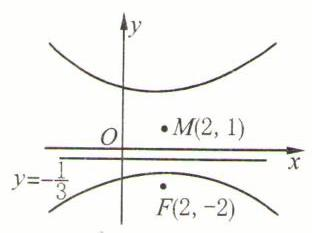
\includegraphics[width=0.2\textwidth]{bodyxb/src/bo_d20aucref24c73anc48g_99_1104_389_312_233_0.jpg}
\end{center}


(图 32)

解 如图 32,双曲线两焦点的连线与 $x$ 轴垂直,故可设双曲线的方程为 $- \dfrac{{\left( x - {x}_{0}\right) }^{2}}{{b}^{2}} + \dfrac{{\left( y - {y}_{0}\right) }^{2}}{{a}^{2}} = 1$ .

$\because$ 焦点 $F\left( {2, - 2}\right)$ 的相应准线为 $y =  - \dfrac{1}{3}$ ,故 $\dfrac{{b}^{2}}{c} = \dfrac{5}{3}$ ,又 $e = \dfrac{c}{a} = \dfrac{3}{2},\therefore$ 可得 $a = 2,b =$  $\sqrt{5},c = 3$ ,于是双曲线的中心为 $M\left( {2,1}\right)$ ,

此双曲线的方程为 $- \dfrac{{\left( x - 2\right) }^{2}}{5} + \dfrac{{\left( y - 1\right) }^{2}}{4} = 1$ .

\begin{center}
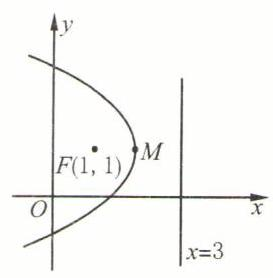
\includegraphics[width=0.2\textwidth]{bodyxb/src/bo_d20aucref24c73anc48g_99_1135_871_273_278_0.jpg}
\end{center}


(图 33)

例 3 求以 $F\left( {1,1}\right)$ 为焦点,准线为 $x = 3$ 的抛物线的方程.

解 显然,抛物线的开口向左 (如图 33),且顶点为 $M\left( {2,1}\right)$ ,故可设抛物线的方程为 ${\left( y - 1\right) }^{2} =  - {2p}\left( {x - 2}\right)$ . 再由焦点 $F\left( {1,1}\right)$ 到准线 $x = 3$ 的距离为 2,得 $p = 2$ ,

$\therefore$ 抛物线的方程为 ${\left( y - 1\right) }^{2} =  - 4\left( {x - 2}\right)$ .

\section*{【训练题】}

(A)

181. 抛物线 ${\left( x + 2\right) }^{2} =  - 4\left( {y - 1}\right)$ 的准线方程是(   )

(A) $y = 2$ . (B) $x = 2$ .

(C) $y = 0$ . (D) $x =  - 3$ .

182. 若椭圆 $8{\left( x - 2\right) }^{2} + k{\left( y - 3\right) }^{2} = {8k}$ 的一条准线为 $y + 1 = 0$ ,则实数 $k$ 的值为 (   )

(A) -4. (B) -1 . (C) 4. (D) 6.

183. 若方程 ${x}^{2} + \left( {k - 1}\right) {y}^{2} - {3ky} + {2k} = 0$ 表示双曲线,则实数 $k$ 的取值范围是 ( )

(A) $\left( {-\infty ,0}\right)$ . (B) $\left( {1, + \infty }\right)$ .

(C) $\left( {-8,0}\right)  \cup  \left( {0,1}\right)$ . (D) $\left( {-\infty , - 8}\right)  \cup  \left( {-8,0}\right)  \cup  \left( {0,1}\right)$ .

184. 双曲线 $9{y}^{2} - {x}^{2} - {2x} - {10} = 0$ 的渐近线方程是(   )

(A) $y =  \pm  3\left( {x + 1}\right)$ . (B) $y =  \pm  3\left( {x - 1}\right)$ .

(C) $y =  \pm  \dfrac{1}{3}\left( {x + 1}\right)$ . (D) $y =  \pm  \dfrac{1}{3}\left( {x - 1}\right)$ .

185. 曲线 $7{\left( x + 1\right) }^{2} - 5{\left( y - 2\right) }^{2} = {35}$ 的离心率是(   )

(A) $\dfrac{\sqrt{74}}{5}$ . (B) $\dfrac{\sqrt{74}}{7}$ . (C) $\dfrac{2\sqrt{15}}{5}$ . (D) $\dfrac{2\sqrt{21}}{7}$ .

186. 焦点为(-3,5),准线为 $y = 7$ 的抛物线方程是(   )

(A) ${\left( y - 6\right) }^{2} =  - 4\left( {x + 3}\right)$ . (B) ${\left( y - 6\right) }^{2} =  - 8\left( {x + 3}\right)$ .

(C) ${\left( x + 3\right) }^{2} =  - 8\left( {y - 6}\right)$ . (D) ${\left( x + 3\right) }^{2} =  - 4\left( {y - 6}\right)$ .

187. 已知抛物线的顶点为(-1,3),对称轴平行于 $y$ 轴,开口向下,其焦点到准线的距离等于椭圆 $\dfrac{{x}^{2}}{25} + \dfrac{{y}^{2}}{9} = 1$ 两准线间的距离,则这个抛物线的方程是 ( )

(A) ${\left( x + 1\right) }^{2} =  - \dfrac{25}{2}\left( {y - 3}\right)$ . (B) ${\left( x + 1\right) }^{2} =  - {25}\left( {y - 3}\right)$ .

(C) ${\left( x - 1\right) }^{2} =  - \dfrac{25}{2}\left( {y + 3}\right)$ . (D) ${\left( x - 1\right) }^{2} =  - {25}\left( {y + 3}\right)$ .

188. 若抛物线 ${y}^{2} = {2px}$ 与 ${y}^{2} = {2q}\left( {x - h}\right) \left( {p,q > 0}\right)$ 有共同的焦点,则 $p,q,h$ 应满足的关系式是(   )

(A) ${2h} = p + q$ . (B) ${2h} =  - \left( {p + q}\right)$ .

(C) ${2h} =  - \left( {p - q}\right)$ . (D) ${2h} = p - q$ .

189. 以 $P\left( {2, - 1}\right) ,Q\left( {2,5}\right)$ 为两顶点,离心率为 3 的双曲线的准线方程是 (   )

(A) $y =  \pm  1$ . (B) $y = 1$ 与 $y = 3$ .

(C) $y = 0$ 与 $y = 4$ . (D) $y =  - \dfrac{2}{3}$ 与 $y = \dfrac{14}{3}$ .

190. 以(2, - 1)与(2,5)为两顶点,以直线 ${3x} - {4y} + m = 0$ 为一条渐近线的双曲线的准线方程是(   )

(A) $x = 2 \pm  \dfrac{9}{5}$ . (B) $y = 2 \pm  \dfrac{9}{5}$ . (C) $x = 2 \pm  \dfrac{16}{5}$ . (D) $y = 2 \pm  \dfrac{16}{5}$ .

191. 与抛物线 ${\left( x - 1\right) }^{2} = 4\left( {y + 1}\right)$ 关于原点对称的图像是(   )

\begin{center}
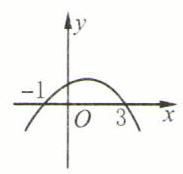
\includegraphics[width=0.2\textwidth]{bodyxb/src/bo_d20aucref24c73anc48g_100_386_1546_183_174_0.jpg}
\end{center}


(A)

\begin{center}
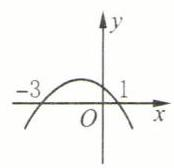
\includegraphics[width=0.2\textwidth]{bodyxb/src/bo_d20aucref24c73anc48g_100_666_1549_174_168_0.jpg}
\end{center}


(B)

\begin{center}
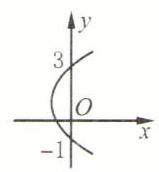
\includegraphics[width=0.2\textwidth]{bodyxb/src/bo_d20aucref24c73anc48g_100_938_1547_159_172_0.jpg}
\end{center}


(C)

\begin{center}
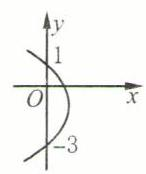
\includegraphics[width=0.2\textwidth]{bodyxb/src/bo_d20aucref24c73anc48g_100_1194_1546_146_174_0.jpg}
\end{center}


(D)

192. (1)椭圆 $4{x}^{2} + 9{y}^{2} + {8x} - {36y} + 4 = 0$ 的中心到直线 ${3x} + {4y} + 1 = 0$ 的距离为\blkda{};

(2)已知椭圆的两条对称轴分别为直线 $x = 5,y + 3 = 0$ ,有一个焦点在 $x$ 轴上,则另一个焦点的坐标是\blkda{}；

(3)圆锥曲线 $3{x}^{2} - {y}^{2} + {6x} + {2y} - 1 = 0$ 的离心率是\blkda{}；

(4)双曲线 ${x}^{2} - {y}^{2} + {8x} + {2y} + {24} = 0$ 的焦点坐标是\blkda{}；

(5)双曲线以直线 $x =  - 1$ 和 $y = 2$ 为对称轴,如果它的一个焦点在 $y$ 轴上,那么它的另一个焦点坐标是\blkda{}；

(6)双曲线 $9{x}^{2} - 4{y}^{2} - {18x} + {8y} - {31} = 0$ 的渐近线方程是\blkda{}；

(7)已知圆锥曲线 $\dfrac{{\left( x - 1\right) }^{2}}{4} + \dfrac{{\left( y - 2\right) }^{2}}{m} = 1$ 的一条准线是 $x = 5$ ,则实数 $m =$ \blkda{}；

(8)已知抛物线 ${y}^{2} = a\left( {x + 1}\right)$ 的准线方程是 $x =  - 3$ ,则其焦点坐标是\blkda{}；

(9)若抛物线 ${\left( y - 1\right) }^{2} = {8x}$ 上的点 $P$ 到其顶点的距离等于点 $P$ 到准线的距离,则点 $P$ 的坐标是\blkda{}.

\section*{(B)}

193. 根据下列条件求椭圆的方程:

(1)以 ${F}_{1}\left( {0, - 1}\right) ,{F}_{2}\left( {0,3}\right)$ 为两个焦点,且过点 $A\left( {2,1}\right)$ ；

(2)中心在点(1, - 2),左焦点是(-3, - 2),右准线方程为 $x = \dfrac{29}{4}$ ；

(3)中心 $\left( {{x}_{0}, - 4}\right)$ 在直线 ${2x} - y + 6 = 0$ 上,焦距是 4,且以曲线 ${x}^{2} + 5{y}^{2} = 5$ 的左准线为右准线;

(4)与椭圆 $\dfrac{{\left( x - 1\right) }^{2}}{16} + \dfrac{{\left( y - 2\right) }^{2}}{9} = 1$ 关于点 $M\left( {-2,1}\right)$ 对称.

194. 根据条件求双曲线的方程:

(1) 离心率是 $e = \dfrac{3}{2}$ ,一个焦点是(2, - 2),其相应的准线方程是 $y =  - \dfrac{1}{3}$ ;

(2)中心在 ${O}^{\prime }\left( {5,6}\right)$ ,一个顶点是(7,6),一个焦点是 $F\left( {1,6}\right)$ ；

(3)两条渐近线为 ${3x} - {4y} = 2$ 和 ${3x} + {4y} = {10}$ ,一条准线为 ${5y} + 4 = 0$ .

195. 根据下列条件, 求抛物线的方程:

(1)焦点为 $F\left( {-2,3}\right)$ ,准线方程为 $y = 6$ ；

(2)顶点在(1,2),对称轴平行于坐标轴,且过点(4,5)；

(3)以曲线 ${y}^{2} - {4x} + {4y} + 8 = 0$ 的焦点为顶点,顶点为焦点；

(4)以 $F\left( {a,b}\right)$ 为焦点,焦点到准线的距离是 $p$ ,且对称轴平行于 $y$ 轴.

\section*{(二) 平移的综合应用}

\section*{【典型题型和解题技巧】}

1. 定义法求轨迹.

例 1 已知 $M\left( {0,6}\right)$ 是圆 ${x}^{2} + {y}^{2} = {100}$ 内的一个定点,求经过点 $M$ 且与已知圆内切的动圆圆心 $P$ 的轨迹方程 (如图 34).

\begin{center}
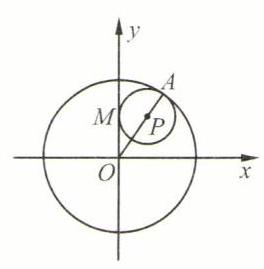
\includegraphics[width=0.2\textwidth]{bodyxb/src/bo_d20aucref24c73anc48g_101_1138_1847_264_269_0.jpg}
\end{center}


(图 34)

解 设圆 $P$ 和圆 ${x}^{2} + {y}^{2} = {100}$ 内切于点 $A$ ,则

$\left| {PO}\right|  + \left| {PM}\right|  = \left| {OA}\right|  = {10},$

由椭圆定义知点 $P$ 在以 $O,M$ 为两个焦点,长轴长为 10 的椭圆上,

于是 ${2a} - {10},{2c} - 6$ ,可得 $b - 4$ ,

又椭圆的中心为(0,3),故点 $P$ 的轨迹方程为 $\dfrac{{x}^{2}}{16} + \dfrac{{\left( y - 3\right) }^{2}}{25} = 1$ .

2. 一元二次方程和圆锥曲线.

(1)直线和圆锥曲线公共点个数的讨论.

例 2 给出定点 $A\left( {3,0}\right) ,B\left( {0,3}\right)$ 和抛物线 $y =  - {x}^{2} + {mx} - 1$ ,求 $m$ 的取值范围,使抛物线和线段 ${AB}$ 恰有一个公共点.

解 线段 ${AB}$ 的方程为 $y = 3 - x\left( {0 \leq  x \leq  3}\right)$ ,代入抛物线方程得 ${x}^{2} - \left( {m + 1}\right) x + 4 = 0$ .

于是问题就归结为上述方程在 $\left\lbrack  {0,3}\right\rbrack$ 内仅有一个实数解. 显然,0 不是该方程的解. 令 $f\left( x\right)$  $= {x}^{2} - \left( {m + 1}\right) x + 4.$

(1)如图 35(1),此时方程有两个相等实数根,且对称轴在 $\left\lbrack  {0,3}\right\rbrack$ 内,

即 $\left\{  \begin{array}{l} \Delta  = 0, \\  \dfrac{m + 1}{2} \in  \left\lbrack  {0,3}\right\rbrack  , \end{array}\right.$ 由此得 $m = 3$ .

(2)如图 35(2),3 不是方程的解,且此时方程恰有一个实数根在(0,3)内,则有 $f\left( 0\right) f\left( 3\right)$  $< 0$ ,

\begin{center}
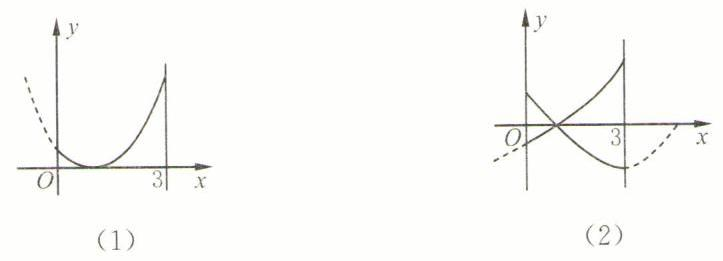
\includegraphics[width=0.6\textwidth]{bodyxb/src/bo_d20aucref24c73anc48g_102_432_975_723_261_0.jpg}
\end{center}


(图 35)

即 $4\left\lbrack  {9 - 3\left( {m + 1}\right)  + 4}\right\rbrack   < 0$ ,由此得 $m > \dfrac{10}{3}$ .

(3)若 $f\left( 3\right)  = 0$ ,则 $m = \dfrac{10}{3}$ ,此时 $f\left( x\right)  = 0$ 的两根为 ${x}_{1} = \dfrac{4}{3},{x}_{2} = 3$ . 与已知矛盾. 综合 (1) , (2)和(3), $m$ 的取值范围是 $m = 3$ 或 $m > \dfrac{10}{3}$ .

注意 本例充分运用了 “数形结合” 的解题技巧, 先把线段和抛物线公共点的讨论, 转化为一元二次方程根的讨论; 然后把方程根的讨论,转化为对抛物线和 $x$ 轴交点位置的要求.

“数形结合”常能使我们从比较复杂的问题中理出清晰的思路,也能从繁冗的计算中得到解脱.

$* \left( 2\right)$ 两条圆锥曲线公共点个数的讨论.

*例 3 椭圆中心为 $\left( {2 + \dfrac{p}{2},0}\right) \left( {p > 0}\right)$ ,焦点在 $x$ 轴上,长半轴、短半轴的长分别为 2 和 1 .

(1)写出椭圆的方程；

(2)若椭圆上有相异四点,各点到椭圆左顶点 $A$ 的距离分别等于该点到直线 $x =  - \dfrac{p}{2}$ 的距离,求 $p$ 的取值范围.

解法一 (1) 椭圆方程为 $\dfrac{{\left\lbrack  x - \left( 2 + \dfrac{p}{2}\right) \right\rbrack  }^{2}}{4} + {y}^{2} = 1$ .

(2)到左顶点 $A\left( {\dfrac{p}{2},0}\right)$ 和到直线 $x =  - \dfrac{p}{2}$ 等距离的点的轨迹是抛物线 ${y}^{2} = {2px}$ .

按题意,椭圆应和抛物线有四个相异公共点,即需方程组 $\left\{  \begin{array}{l} {y}^{2} = {2px}, \\  {\left\lbrack  x - \left( 2 + \dfrac{p}{2}\right) \right\rbrack  }^{2} + {y}^{2} = 1 \end{array}\right.$ 有相异四组解,消去 $y$ ,并整理得 ${x}^{2} + \left( {{7p} - 4}\right) x + \dfrac{{p}^{2}}{4} + {2p} = 0$ .

注意到 ${y}^{2} = {2px}$ 的图形,上述方程应有相异的两个正数解,故需

$\left\{  {\begin{array}{l} \Delta  > 0, \\  {x}_{1} + {x}_{2} > 0, \\  {x}_{1}{x}_{2} > 0, \end{array}\text{ 即 }\left\{  {\begin{array}{l} {\left( 7p - 4\right) }^{2} - 4\left( {\dfrac{{p}^{2}}{4} + {2p}}\right)  > 0, \\  4 - {7p} > 0, \\  {x}_{1}{x}_{2} > 0, \end{array}\text{ 即 }\left\{  {\begin{array}{l} p > 1\text{ 或 }p < \dfrac{1}{3}, \\  p < \dfrac{4}{7}, \\  p <  - 8\text{ 或 }p > 0. \end{array}\therefore 0 < p < \dfrac{1}{3}.}\right. }\right. }\right.$

解法二 令 $f\left( x\right)  = {x}^{2} + \left( {{7p} - 4}\right) x + \dfrac{{p}^{2}}{4} + {2p}$ .

\begin{center}
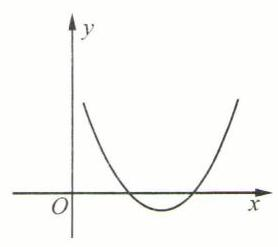
\includegraphics[width=0.2\textwidth]{bodyxb/src/bo_d20aucref24c73anc48g_103_1158_997_278_247_0.jpg}
\end{center}


(图 36)

为使已得方程有两相异正数解,只需抛物线 $y = f\left( x\right)$ 和 $x$ 正半轴有

两相异公共点 (如图 36),于是 $\left\{  \begin{array}{l} f\left( 0\right)  > 0, \\  \Delta  > 0, \\  \text{ 对称轴 }x =  - \dfrac{{7p} - 4}{2} > 0. \end{array}\right.$

(下略)

\section*{【训练题】}

\section*{(A)}

196. 到 $y$ 轴的距离与到点 $A\left( {2,0}\right)$ 的距离相等的点的轨迹方程是 (   )

(A) ${y}^{2} =  - 2\left( {x - 1}\right)$ . (B) ${x}^{2} =  - 2\left( {y - 1}\right)$ .

(C) ${y}^{2} = 4\left( {x + 1}\right)$ . (D) ${y}^{2} = 4\left( {x - 1}\right)$ .

*197. 已知曲线 ${x}^{2} - {y}^{2} + 1 = 0$ 与 ${y}^{2} = \left( {k - 1}\right) x$ 有且只有两个不同的公共点,则实数 $k$ 的取值范围是(   )

(A) $k =  - 1$ 或 $k = 3$ . (B) $k = 1$ 或 $k =  - 3$ .

(C) $- 1 < k < 3$ . (D) $k <  - 1$ 或 $k > 3$ .

$* {198}$ . 椭圆 $\dfrac{{\left( x + 1\right) }^{2}}{4} + {y}^{2} = 1$ 和抛物线 ${\left( x + 1\right) }^{2} = 1 - y$ 的公共点个数是 (   )

(A) 1 . (B) 2 . (C) 3 . (D) 4 .

* 199. 已知集合 $M = \left\{  {\left( {x,y}\right)  \mid  4{x}^{2} + {\left( y - a\right) }^{2} = 4}\right\}  ,P = \left\{  {\left( {x,y}\right)  \mid  y = \dfrac{1}{2}{x}^{2}}\right\}$ ,满足 $M \cap  P \neq  \varnothing$ ,则实数 $a$ 的取值范围是 (   )

(A) $\left( {-\infty ,\dfrac{5}{2}}\right\rbrack$ . (B) $\left\lbrack  {-2,\dfrac{5}{2}}\right\rbrack$ . (C) $\left\lbrack  {-2,2}\right\rbrack$ . (D) $\left\lbrack  {2,\dfrac{5}{2}}\right\rbrack$ .

200. 以抛物线 ${\left( y + 1\right) }^{2} = 8\left( {x - 2}\right)$ 上任一点 $P$ 为圆心作与 $y$ 轴相切的圆,则这些圆必过定点(   )

(A)(2, - 1). (B)(4, - 1). (C)(6, - 1). (D)(8, - 1).

\section*{(B)}

201. 若抛物线 $y = a{x}^{2} - 1$ 上存在关于直线 $x + y = 0$ 对称的相异两点,试求 $a$ 的取值范围.

202. 过原点作两条互相垂直的直线交抛物线 ${y}^{2} = {4p}\left( {x + p}\right) \left( {p > 0}\right)$ 得两条弦 ${AB},{CD}$ ,求 $\left| {AB}\right|  + \left| {CD}\right|$ 的最小值.

*203. 已知抛物线 $y = {x}^{2} - 2$ 与椭圆 $\dfrac{{x}^{2}}{4} + {y}^{2} = 1$ ,求证:

(1)抛物线和椭圆有四个不同的公共点；

(2)这四个公共点在同一个圆上,并求出该圆的方程.

204. (1) 求 $a$ 的取值范围,使椭圆 $2{x}^{2} + {\left( y - a\right) }^{2} - 2 = 0$ 上恰好有两点到 $x$ 轴及到点(0,1)的距离相等;

\begin{center}
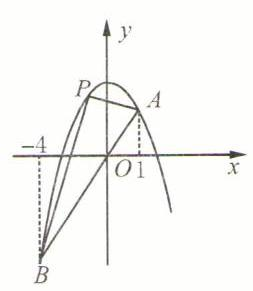
\includegraphics[width=0.2\textwidth]{bodyxb/src/bo_d20aucref24c73anc48g_104_1200_1059_253_291_0.jpg}
\end{center}


(第 205 题)

$* \left( 2\right)$ 设椭圆 ${x}^{2} + 4{y}^{2} = 4$ 和抛物线 ${x}^{2} = y - m$ 有四个相异公共点,求 $m$ 的取值范围.

205. 已知抛物线 $y = 4 - {x}^{2}$ 与直线 $y = {3x}$ 相交于 $A,B$ 两点,又点 $P$ 沿抛物线由点 $A$ 到点 $B$ 运动 (如图).

(1)求当 $\bigtriangleup {PAB}$ 面积最大时点 $P$ 的坐标；

(2)设与线段 ${AB}$ 平行的直线和抛物线交于 $C,D$ 两点,求证: 线段 ${CD}$ 恒被定直线 $x =$  ${x}_{0}$ 分成两等分.

206. 已知过原点 $O$ 的直线 $l$ 与曲线 ${y}^{2} = 4\left( {x - 1}\right)$ 交于 $A,B$ 两点,以 ${AB}$ 为直径的圆恰好过上述曲线的焦点 $F$ (如图).

\begin{center}
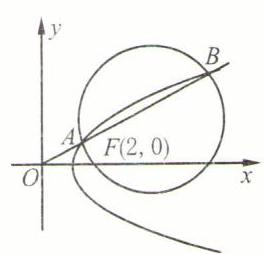
\includegraphics[width=0.2\textwidth]{bodyxb/src/bo_d20aucref24c73anc48g_104_1189_1571_264_254_0.jpg}
\end{center}


(第 206 题)

(1)求直线 $l$ 的方程；

(2)求 $\left| {AB}\right|$ 的值.

207. (1) 已知 $\bigtriangleup {ABC}$ 的两个顶点 $A,B$ 是椭圆 $\dfrac{{\left( x - 2\right) }^{2}}{169} + \dfrac{{\left( y + 1\right) }^{2}}{25} = 1$ 的两个焦点,顶点 $C$ 在曲线 $y = {x}^{2}$ 上,求这个三角形重心的轨迹方程;

(2)已知动圆和圆 ${x}^{2} + {y}^{2} = 4{r}^{2}$ 内切、和圆 ${\left( x - r\right) }^{2} + {y}^{2} = {r}^{2}\left( {r > 0}\right)$ 外切,求动圆圆心 $M$ 的轨迹方程;

(3)已知动圆和圆 ${x}^{2} + {y}^{2} = 1,{x}^{2} + {y}^{2} - {8x} + 7 = 0$ 都内切,求动圆圆心 $M$ 的轨迹方程；

(4)已知动圆和圆 ${\left( x + 2\right) }^{2} + {y}^{2} = 4$ 外切,并与直线 $x = 2$ 相切,求动圆圆心 $M$ 的轨迹方程；

(5)已知椭圆一个焦点为 $O\left( {0,0}\right)$ ,且过 $\left( {-5,{12}}\right) ,\left( {9,{12}}\right)$ 两点,求椭圆的另一个焦点 $F$ 的轨迹方程.

208. 已知动圆 $M$ 过定点 $A\left( {3,0}\right)$ ,且截 $y$ 轴正向 (即 $y \geq  0$ ) 所得的线段 ${BC}$ 保持定长 ${2a}$ ,求动圆圆心 $M$ 的轨迹方程,并说明轨迹是什么图形.

209. 已知一抛物线过定点 $A\left( {0,2}\right)$ ,且以 $x$ 轴为准线 (如图).

\begin{center}
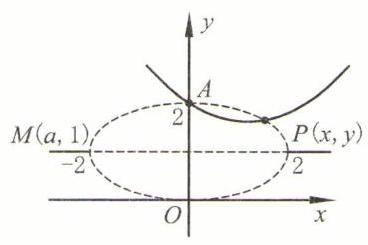
\includegraphics[width=0.3\textwidth]{bodyxb/src/bo_d20aucref24c73anc48g_105_1089_359_368_245_0.jpg}
\end{center}


(第 209 题)

(1)求此抛物线顶点 $P$ 的轨迹(记作 $C$ )方程；

(2)若点 $M\left( {a,1}\right)$ 不在线段 $y = 1\left( {-2 \leq  x \leq  2}\right)$ 上,试求实数 $a$ 的值,使得过点 $M$ 存在一对互相垂直的直线,且这对直线同时与曲线 $C$ 有公共点.

210. (1) 已知双曲线经过点 $M\left( {2,3}\right)$ ,并以 $y$ 轴为右准线,其虚轴长、实轴长和焦距依次成等差数列,求双曲线的右焦点 $P$ 的轨迹方程;

(2)求离心率为 $\dfrac{1}{2}$ ,一条准线方程为 $x + 2 = 0$ ,恒过定点 $M\left( {1,0}\right)$ ,且使长轴长最大的椭圆方程.

211. 一双曲线的右顶点在抛物线 ${y}^{2} = x - 1$ 上,右准线是 $y$ 轴,实轴长是 4,求:

(1)此双曲线中心的轨迹； (2)离心率最小时的双曲线方程.

212. 已知椭圆 ${x}^{2} + \dfrac{{y}^{2}}{{\tan }^{2}\alpha } = 1$ ( $\alpha$ 为锐角) 的焦点在 $x$ 轴上, $A$ 是它的右顶点,椭圆与射线 $y = x$  $\left( {x \geq  0}\right)$ 的公共点是 $B$ ,以 $A$ 为焦点,过点 $B$ 且开口向左的抛物线的顶点为(m,0)(如图),当椭圆的离心率 $e$ 在 $\left( {\dfrac{\sqrt{6}}{3},1}\right)$ 中变化时,求 $m$ 的取值范围.

\begin{center}
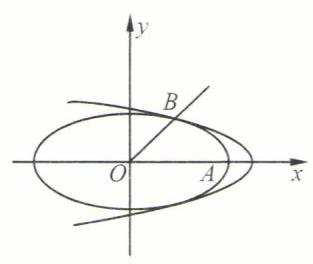
\includegraphics[width=0.2\textwidth]{bodyxb/src/bo_d20aucref24c73anc48g_105_408_1321_313_264_0.jpg}
\end{center}


(第 212 题)

\begin{center}
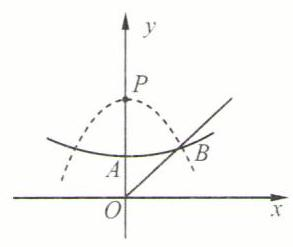
\includegraphics[width=0.2\textwidth]{bodyxb/src/bo_d20aucref24c73anc48g_105_851_1338_293_247_0.jpg}
\end{center}


(第 213 题)

213. 已知 $A$ 是双曲线 $\dfrac{\left( {1 - {a}^{2}}\right) {x}^{2}}{{a}^{2}} + {y}^{2} = 1\left( {a > 0}\right)$ 的上支顶点, $B$ 是其上支与直线 $y = x$ 的交点 (如图),当其一条渐近线的斜率在区间 $\left\lbrack  {\dfrac{\sqrt{3}}{2},\dfrac{2\sqrt{2}}{3}}\right\rbrack$ 上变化时,求过点 $B$ 、以点 $A$ 为焦点且关于 $y$ 轴对称的抛物线顶点 $P$ 的纵坐标的取值范围.

\section*{(C)}

214. 若关于 $x$ 的方程 $\sqrt{1 - {x}^{2}} = {mx} + 1$ 有且仅有一个实数解,求实数 $m$ 的值.

215. (1) 已知实数 $x,y$ 满足 ${\left( x - 4\right) }^{2} + {\left( y - 3\right) }^{2} = 4$ ,试分别求 $u = {\left( x - 6\right) }^{2} + {\left( y + 2\right) }^{2}$ 和 $v =$  $\dfrac{y + 3}{x + 6}$ 的取值范围;

(2)已知实数 $x,y$ 满足 $x \geq  1,y \geq  1,{\log }_{a}^{2}x + {\log }_{a}^{2}y = {\log }_{a}\left( {a{x}^{2}}\right)  + {\log }_{a}\left( {a{y}^{2}}\right) (a > 0,a \neq$ 1),求 ${\log }_{a}\left( {xy}\right)$ 的取值范围;

(3)在半径为 $a$ ,圆心角为 ${90}^{ \circ  }$ 的扇形 ${OAB}$ 的弧 ${AB}$ 上有一动点 $P$ ,过点 $P$ 作 ${OA}$ 的垂线,垂足为 $H$ (如图). 当点 $P$ 沿圆弧从点 $B$ 运动到点 $A$ 时, $\bigtriangleup {OPH}$ 的内心 $Q$ 的轨迹是什么曲线, 并求出这段曲线长.

\begin{center}
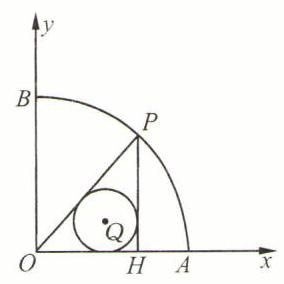
\includegraphics[width=0.2\textwidth]{bodyxb/src/bo_d20aucref24c73anc48g_106_426_590_284_284_0.jpg}
\end{center}


[第 215(3)题]

\begin{center}
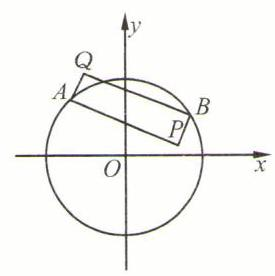
\includegraphics[width=0.2\textwidth]{bodyxb/src/bo_d20aucref24c73anc48g_106_902_590_275_276_0.jpg}
\end{center}


(第 216 题)

216. 已知 $P\left( {a,b}\right)$ 是圆 ${x}^{2} + {y}^{2} = {r}^{2}$ 内的一个定点, $A,B$ 是圆上的动点,且满足 $\angle {APB} = {90}^{ \circ  }$ (如图),求矩形 ${APBQ}$ 的顶点 $Q$ 的轨迹方程.

217. 已知曲线 ${x}^{2} + \dfrac{{y}^{2}}{2} = {a}^{2}\left( {a > 0}\right)$ 与连接 $A\left( {-1,1}\right) ,B\left( {2,3}\right)$ 的线段 ${AB}$ 没有公共点,求 $a$ 的取值范围.

\begin{center}
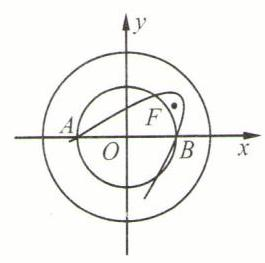
\includegraphics[width=0.2\textwidth]{bodyxb/src/bo_d20aucref24c73anc48g_106_1194_1073_265_263_0.jpg}
\end{center}


(第 218 题)

218. 已知两个同心圆,其半径分别为 $a,r\left( {a > r}\right) ,{AB}$ 为小圆上的一条定直径 (如图),求以大圆切线 $l$ 为准线,且过 $A,B$ 两点的抛物线的焦点 $F$ 的轨迹方程.

219. 已知动点 $A,B$ 在直线 $x = 3$ 上移动,且 $\angle {AOB} = \dfrac{\pi }{3}$ ( $O$ 为原点),求 $\bigtriangleup {AOB}$ 外心 $M$ 的轨迹方程.

220. 一动点 $P$ 到一定点 $F\left( {-c,0}\right) \left( {c \geq  0}\right)$ 的距离等于它到定圆 ${\left( x - c\right) }^{2} + {y}^{2} = 4{r}^{2}$ 上的点的最短距离,试求动点 $P$ 的轨迹方程.

221. 半圆的直径 $\left| {AB}\right|  = {2R}$ ,半圆外的直线 $l$ 与 ${BA}$ 延长线垂直,垂足为 $T$ ,且 $\left| {AT}\right|  = {2a}$  $\left( {{2a} < \dfrac{R}{2}}\right)$ . 半圆上有相异两点 $M,N$ ,它们到 $l$ 的距离分别为 ${d}_{1},{d}_{2}$ ,且 ${d}_{1} = \left| {AM}\right| ,{d}_{2} =$  $\left| {AN}\right|$ . 求证: $\left| {AM}\right|  + \left| {AN}\right|  = {2R}$ .

222. 已知 ${PQ}$ 是圆 ${x}^{2} + {y}^{2} = {r}^{2}$ 中与 $x$ 轴垂直的一条定弦 (非直径,如图). 求证: 所有被 ${PQ}$ 平分的弦所在的直线都与同一条抛物线仅有一个公共点.

\begin{center}
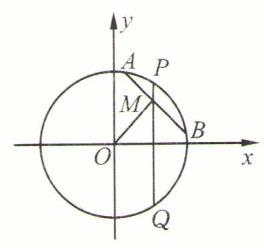
\includegraphics[width=0.2\textwidth]{bodyxb/src/bo_d20aucref24c73anc48g_106_1200_1863_264_248_0.jpg}
\end{center}


(第 222 题)